\documentclass[12pt,a4paper,twoside,openright,headinclude,liststotoc,bibtotoc]{scrreprt}
\usepackage[english,ngerman]{babel}
%---um mehrsprachige Texte zu verfassen, daher zwei folgende Pakete
\usepackage{ucs} 
\usepackage[utf8x]{inputenc}
%---calc erlaubt einfaches Rechnen
\usepackage{calc}
\usepackage{exscale}
\usepackage{textcomp}
\usepackage{scrpage2}
%---zur Erstellung von Tabellen, erweiterte Version von tabular*
\usepackage{tabularx}
%---fuer Graphiken
\usepackage{longtable}
\usepackage{wrapfig}
%---zum Zitieren von Referenzen innerhalb des Textes!????(Zitate,????)
\usepackage{varioref}
%---um jm. zu zitieren, anders als mit dem Paket natbib
\usepackage{url}
\usepackage{units}
%\usepackage{a4wide}
\usepackage[usenames]{color}
\usepackage{listings}
\usepackage{alltt}
\usepackage{graphicx}
%%%%%%%%%%%%%%%%%%%%%%%%%\usepackage[dvips]{graphicx}
\usepackage{epsfig}
\usepackage{pslatex}
\usepackage{latexsym}
\usepackage{amsmath}
\usepackage{textcomp}
%---erlaubt Trennung von Woertern, die Umlaute enthalten
\usepackage[T1]{fontenc}
\usepackage{float}
%%%%%%%%%%%%%%%%%%%%%%%%%\usepackage[bf]{caption}``normales'' Package für Caption
\usepackage[labelsep=period]{caption}
%\usepackage[latin1]{inputenc}
%---kombiniert 3 verschiedene Bibliographie Stile (zitieren)
\usepackage[round]{natbib}
\setlength{\textheight}{23cm}
\setlength{\textwidth}{17cm}
%\setlength{\topmargin}{-1cm}
%\setlength{\oddsidemargin}{0cm}
%\setlength{\evensidemargin}{0cm}
%\setlength{\topmargin}{0cm}
\addtolength{\oddsidemargin}{-5pt}
\addtolength{\evensidemargin}{-40pt}
%%%%%%%%%%%%%%%%%%5\setlength{\headsep}{0.4cm}
\setlength{\topmargin}{1cm}
\allowdisplaybreaks
\setlength{\parindent}{0em}
\setlength{\parskip}{1.1ex}
%existierender Befehl wird veraendert
\renewcommand{\baselinestretch}{1.025}
%erzeugt einen neuen Befehl; Syntax: \newcommand{\befehl}[narg][standard]{def.}
%narg :optionaler Parameter, darf alle Werte zw. 1 und 9 annehmen, bestimmt
%Anzahl der moegl. Argumente fuer den zu definierenden Befehl
% standard : 2. optionaler Parameter 
\newcommand{\equref}[1]{(\ref{#1})}
%Seitenlayout, headings: 
\pagestyle{scrheadings}
\manualmark
%\automark[section]{chapter}
%\setheadsepline{0.4pt}[\color{black}]
\addtokomafont{caption}{\small}
\setkomafont{captionlabel}{\normalfont\bfseries}
\setcounter{secnumdepth}{3}
\setcounter{tocdepth}{2}
%sorgt dafuer,dass kein Ausgleich des unteren Seitenrandes durch Dehnung der 
% Absatzabstände durchgeführt wird
\raggedbottom
%
%abkürzungsverzeichnis
\usepackage{nomencl}
\let\abbrev\nomenclature
\renewcommand{\nomname}{Abkürzungsverzeichnis}
\setlength{\nomlabelwidth}{.25\hsize}
\renewcommand{\nomlabel}[1]{#1 \dotfill}
\setlength{\nomitemsep}{-\parsep}
\makeglossary
\usepackage[normalem]{ulem}
\newcommand{\markup}[1]{\uline{#1}}
\begin{document}
%% Titelseite ausgeben
\begin{titlepage}
%\pagenumbering{roman}
%% Den ganzen Text auf der Titelseite zentrieren
\begin{center}
%\vspace{2.0cm}

\huge Planet Simulator Climate
\vspace{1cm}

%\huge Meteorologisches Institut, Universität Hamburg

%\vspace{0.5cm}

\vspace{1cm}

\begin{figure}[H]
\begin{tabular}{cc}
\begin{minipage}{1.0\textwidth}
\begin{center}
\includegraphics[height=10.0cm]{eps/mstream_anm_2new.eps}
\end{center}
\end{minipage}
\end{tabular}
\caption*{\begin{scriptsize}PlaSim annual mean meridional-height cross-section\end{scriptsize}}            
\end{figure} 

\vspace{1cm}

%Namen
\large
Meteorologisches Institut, Universität Hamburg\\
\vspace{1cm} 
Kerstin Haberkorn, Frank Sielmann, Frank Lunkeit, Edilbert Kirk, Andrea Schneidereit, Klaus Fraedrich


\vspace{2cm}

\end{center}
\end{titlepage}
%%%%%%%%%%%%%%\pagestyle{empty}
\pagenumbering{arabic}
\linespread{1.0}
%\linespread{1.67}
\small\normalsize
\selectlanguage{english}
\chapter*{Abstract}
\vspace{-0.4cm}

The Planet Simulator (PlaSim) is a general circulation model on its way to a user friendly tool for climate research. Its analysis is based on a 50 year control run with prescribed sea surface temperature climatology taken from AMIP (Atmospheric Model Intercomparison Project). The control run is confined to the atmospheric part without interaction with the subcomponents, and the diagnostics is compared with reanalysis data ERA-40 (\underline{E}uropean \underline{C}enter for \underline{M}edium Range \underline{W}eather \underline{F}orecast reanalysis). Results highlight similarities with and deviations from observations: Global energetics and spatial distributions of the first and second moments of the climate variables appear to be well represented. Main differences occur in the polar regions, which show a cold bias and, subsequently, stationary wave patterns reveal too strong zonality. The atmospheric module of the next PlaSim version includes (i) a new surface presentation (with sea ice, land surface etc), (ii) re-evaporation of precipitation, (iii) gravity wave drag, and (iv) the diurnal cycle. Planet Simulator Climate supplements the Manual and the Users’ Guide and is available from \url{http://www.mi.uni-hamburg.de/Downloads-and-related-papers.245.0.html}.


\setlength{\headsep}{0.4cm}
\setlength{\topmargin}{-2cm}
  
\tableofcontents
%\linespread{1.0}
\small\normalsize
\newpage
%\listoffigures
%\listoftables
%\pagenumbering{arabic}

%\setlength{\headsep}{0.4cm}
%\setlength{\topmargin}{-2cm}
  
\vspace{-0.4cm}
\chapter{Planet Simulator: Control run climatology}
\vspace{-0.4cm}

The climate of the PlaSim control run (50 years) is analysed and the results are compared with observations (ERA reanalysis and other data). The climatology is presented in terms of global means, meridional-height cross-sections and two-dimensional circumpolar or global maps (with meridional profiles of zonal means) of key atmospheric variables. Besides 30 year annual means, the main seasons of winter (DJF) and summer (JJA) are also presented including intraseasonal variability. 

\vspace{-0.4cm}
\section{Planet Simulator (PlaSim)}
\vspace{-0.4cm}
The Planet Simulator (PlaSim) is a {\underline{G}eneral \underline{C}irculation \underline{M}odel} (GCM), whose dynamical core for the atmosphere is adopted from PUMA (\underline{P}ortable \underline{U}niversity \underline{M}odel of the \underline{A}tmosphere). The model is based on the moist primitive equations conserving momentum, mass, energy and moisture. Besides the atmospheric part, other climate subsystems are included with highly reduced dynamics: a land surface with biosphere and a mixed layer-ocean with sea ice (for details see PlaSim Reference Manual \citet{Lunkeit2007a}, for an overview see \citet{Fraedrich2005aa}). A control run for a period of 50 years is performed with PlaSim based on T21 resolution with ten vertical, non-equidistant levels in $\sigma$-coordinates ($\sigma=p/p_{s}$). A fixed composition of the atmosphere is used, the annual cycle is included but not the diurnal. The default parameters used (see appendix) are the following: a year with 365 days (and 366 for leap years), the solar constant of 1365 ${Wm^{-2}}$, $CO_{2}$-content of 348 ppmv and the time step (MPSTEP) = 45 minutes. To make PlaSim comparable to AMIP (\underline{A}tmospheric \underline{M}odel \underline{I}ntercomparison \underline{P}roject), the sea surface temperatures of the AMIP II-period (1979 to 1996) are used to provide the climatological annual cycle. In addition, the distribution of sea ice and all other subsystems are prescribed by climatological means; they are not used interactively.

\vspace{-0.4cm}
\section{ERA-40 reanalysis}
\vspace{-0.4cm}
The PlaSim simulation is compared with the ERA-40 European Center for Medium-Range Weather Forecasts (ECMWF) reanalysis data. This data set spans the period 1957 to 2002 (a comprehensive description can be found in \citet {Kaallberg2005}, \citet{Gibson1997} and \citet{Simmons2000}), is available from \url{http://data.ecmwf.int/data/d/era40_moda/} and is widely used for model validation and research. In contrast to PlaSim, the horizontal resolution of ERA-40 (called ERA hereinafter) is 144 $\times$ 73 grid boxes (PlaSim: 64 $\times$ 32), which requires interpolation to make the data comparable. Monthly means are derived from daily means of a six hourly data set. 

\vspace{-0.4cm}
\section{Presentation}
\vspace{-0.4cm}
The PlaSim seasonal and annual mean climate are presented by first and second moments of variables characterising radiative, thermal, dynamic and moisture processes. This includes state variables, eddy fluxes and other derived quantities (wavenumber-frequency spectra  etc.) of atmospheric dynamics. The climate is presented by the following set of displays:  
(i) Global and annual mean energetics: Here we present the thermal forcing in terms of solar and terrestrial radiative, latent and sensible heat fluxes, the water cycle, and the Lorenz energy cycle.\\
(ii) Meridional-height cross-sections provide zonally averaged fields of the primary and secondary circulation with temperature, zonal wind and mass streamfunction. This is supplemented by zonally averaged eddy heat and momentum fluxes and, as a combination, by fluxes of transient and stationary wave activity (Eliassen-Palm flux), and the Eulerian mean flow.\\
(iii) Fields are presented for the surface (radiation, mass, temperature, sensible and latent heat fluxes, precipitation) and, for radiative fluxes, also at the top of the atmosphere; lower and upper tropospheric fields show the dynamical variables. Almost all fields include meridional profiles (right panels) of the respective zonal averages. Information on mid-latitude and tropical cyclones supplement the analysis: mid-latitude cyclone density is obtained from cyclone-track detection and the seasonal tropical cyclogenesis parameter is adopted.\\
(iv) Global surface climates are classified based on \citet{Koeppen1936} and the Budyko-Lettau index of dryness \citep{Budyko1958,Lettau1969}.\\


\vspace{-0.4cm}
\chapter{Global energetics}
\vspace{-0.4cm}
\section{Energy budget}
\vspace{-0.4cm}

The global balance of energy fluxes (Fig. \ref{img:enercycle} a) consists of the following components: solar and terrestrial radiation at top and bottom of the atmosphere and latent and sensible heat. PlaSim shows good agreement with the observations \citep{Kiehl1997}: The incoming solar radiation for PlaSim is 341 $W/m^2$ (compared to 342 $W/m^2$); the absorbed and reflected fluxes in the atmosphere yield 64 and 74 $W/m^2$ (67 and 77 $W/m^2$) and at the surface 31 and 172 $W/m^2$ (30 and 168 $W/m^2$). PlaSim underestimates sensible heat flux with 20 $W/m^2$ (24 $W/m^2$) and overestimates latent heat flux with 91 $W/m^2$ (78 $W/m^2$). The surface terrestrial radiation is captured very well (389 compared to 390 $W/m^2$). The longwave outgoing and atmospheric counter radiation are somewhat larger with 239 and 328 $W/m^2$ (compared to 235 $W/m^2$) and 324 $W/m^2$).


\vspace{-0.4cm}
\section{Water budget}
\vspace{-0.4cm}

The global water budget (Fig. \ref{img:enercycle} b) describes continental and oceanic precipitation, evaporation and the transports by the atmosphere and river runoff (units in $kg/m^{2}$). There is good agreement with observations \citep{Trenberth2006}: oceanic precipitation and evaporation (precipitation: 443 compared to 373 $kg/m^{2}$, evaporation: 473 and 413 $kg/m^{2}$) as well as continental (precipitation: 142 compared to 113 $kg/m^{2}$, evaporation: 112 and 73 $kg/m^{2}$) are both overestimated by PlaSim whereas the atmospheric transport and the surface runoff are slightly underestimated (30 compared to 40 $kg/m^{2}$).

\vspace{-0.4cm}
\section{Lorenz energy cycle}
\vspace{-0.4cm}

The Lorenz energy cycle presents the global energy balance, which includes reservoirs relevant for atmospheric dynamics, energy  fluxes into and conversions between them. The Lorenz cycle is commonly displayed as a box scheme (Fig. \ref{img:lez}), describing the reservoirs of available potential (ZPE) and  kinetic energy (ZKE) of the zonal mean flow, available potential energy of the transient (TPE) and stationary (SPE) eddies and kinetic energy of transient (TKE) and stationary eddies (SKE). Sources, sinks and conversions are symbolised by arrows. The energy of eddies and their conversion terms can be partitioned in three categories: The long waves (LW) include all wavenumbers smaller than four, synoptic waves (SW) represent four to nine, and small wavenumbers (KW) from 10 to 21. The reservoir of available potential energy of the zonal mean flow is largest. It is transformed to eddy available potential (by transient and stationary eddies), and to zonal mean kinetic energy, which is small with Ferrel and Hadley cell %contributions almost cancelling \citep[p. 383]{Peixoto1993} and \citep[p. 341]{Holton1992}.
contributions almost cancelling (\citet[p. 383]{Peixoto1993} and \citet[p. 341]{Holton1992}).

\begin{figure}[c]
\begin{tabular}{cc}
\begin{minipage}{1.0\textwidth}\hspace{1.15cm}\begin{scriptsize}(a)\end{scriptsize} \vspace{-0.15cm}
\begin{center}
\includegraphics[height=9.0cm]{eps/heat.eps}
\end{center}
\end{minipage}
\\
\\
\\
\begin{minipage}{1.0\textwidth}\hspace{1.15cm}\begin{scriptsize}(b)\end{scriptsize} \vspace{-0.15cm}
\begin{center}

\includegraphics[height=9.0cm]{eps/water.eps}
\end{center}
\end{minipage}
\end{tabular}
\caption[PlaSim global and annual mean energy and water budgets]{PlaSim global and annual mean energy and water budgets; (a) Energy, units in [$W/m^2$], (b) Water, units in [$kg/m^{2}$]}
\label{img:enercycle}
\end{figure}


\begin{figure}[c]
\begin{tabular}{cc}
\begin{minipage}{1.0\textwidth}
\begin{center}
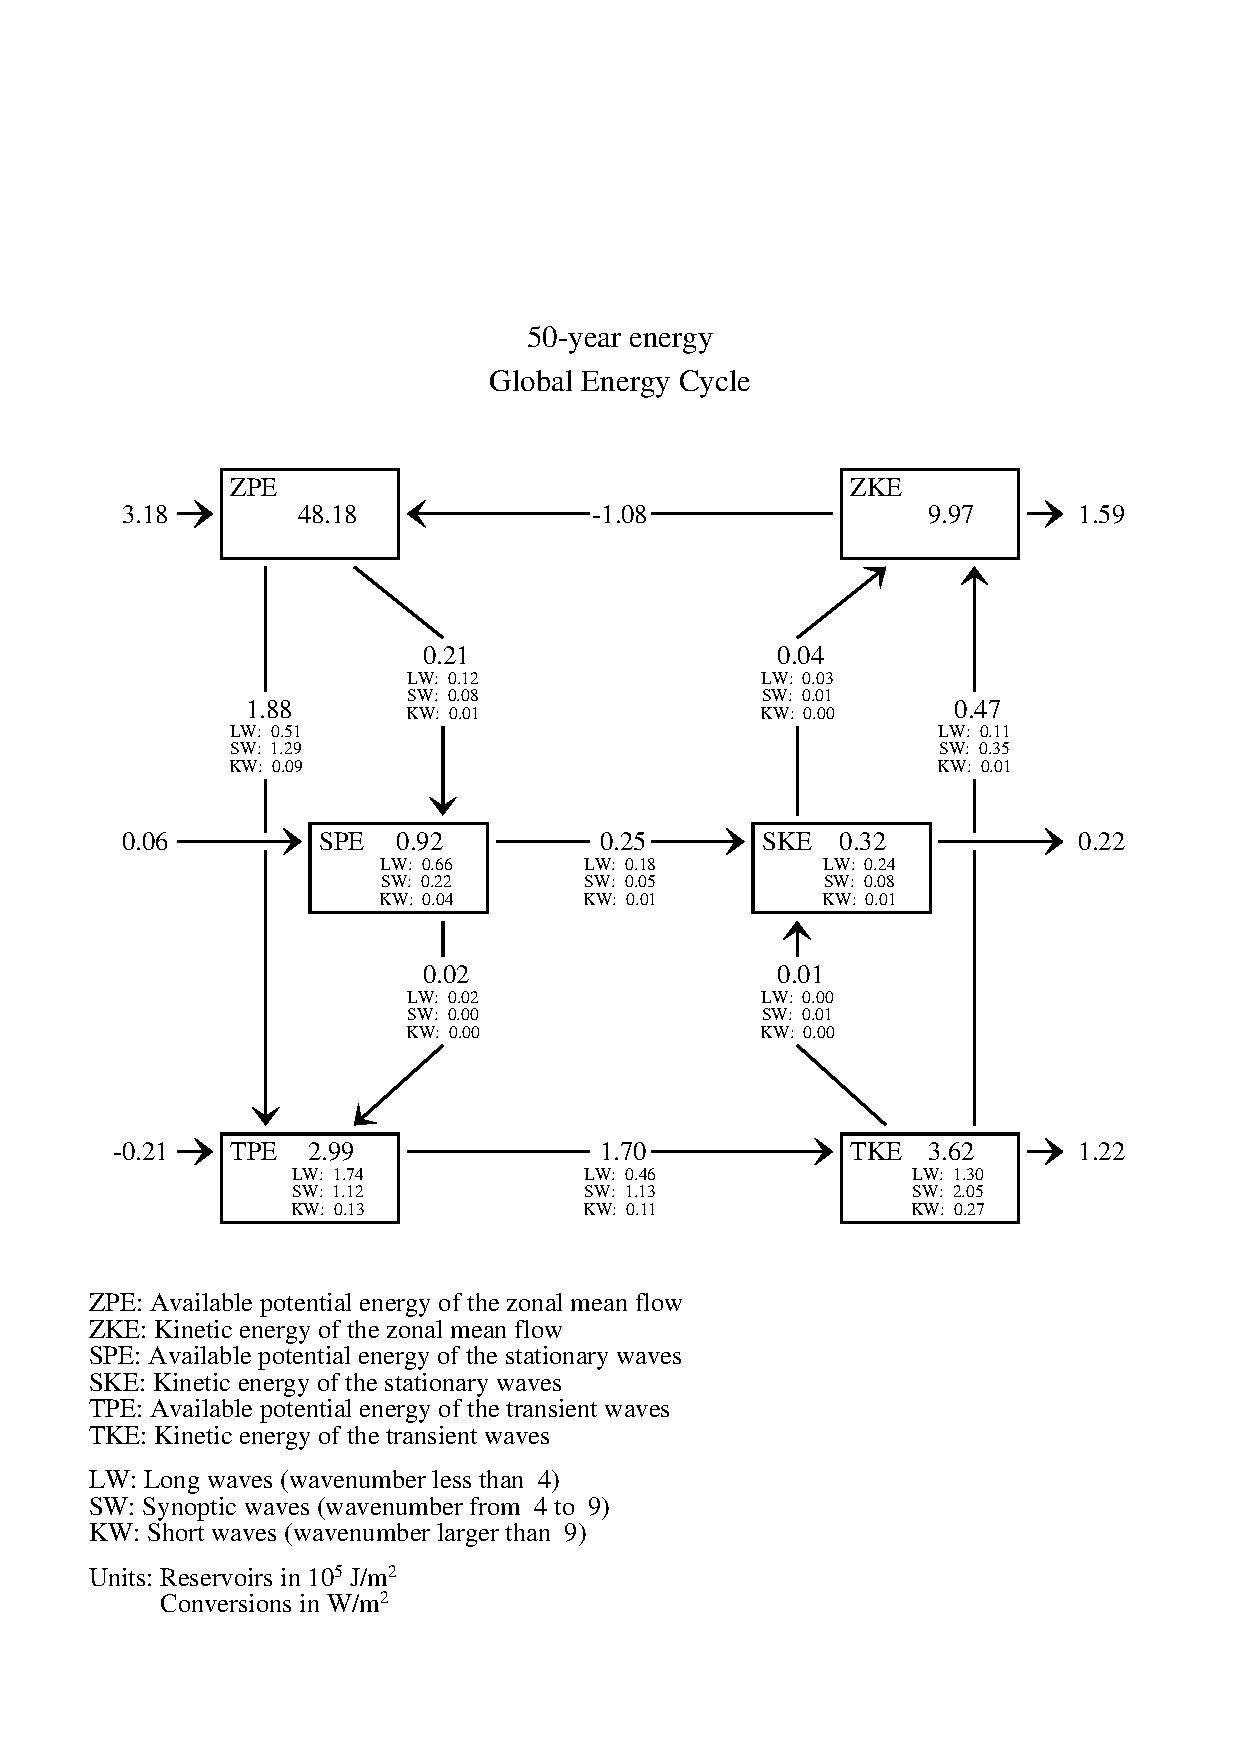
\includegraphics[height=19.0cm]{eps/LEZANM.epsi}
\end{center}
\end{minipage}
\end{tabular}
\vspace{-5.2cm}\caption[Global and annual mean Lorenz energy cycle]{Global and annual mean Lorenz energy cycle, reservoirs in $10^{5}J/m^{2}$, conversions in $W/m^{2}$}
\label{img:lez}
\end{figure}

\vspace{-0.4cm}
\chapter{Zonal averages: temperature, zonal wind, mass streamfunction}
\vspace{-0.4cm}
Meridional-height cross-sections show zonal averages of temperature and zonal wind (Fig. \ref{img:tuall}) and the mass streamfunction (Fig. \ref{img:streamfct}) for seasonal and annual means characterising primary and secondary circulation.

\vspace{-0.4cm}
\section{Temperature and zonal wind}
\vspace{-0.4cm}

PlaSim reveals the typical patterns of the temperature distribution and the associated zonal winds with mid-latitude westerlies and easterlies in equatorial regions. The subtropical jets are situated near 30°-35° in winter with jetstream-axes located below the tropopause at 200 hPa. The wind maxima shift polewards to about 40°-45° during summer. These characteristics are captured by PlaSim and ERA (Fig. \ref{img:tuall} a, d). Compared to ERA, PlaSim tends to slightly overestimate the jet maxima (PlaSim: 40 $m/s$, ERA: 35 $m/s$) associated with a more upward and poleward location. In SH winter (Fig. \ref{img:tuall} b, e), the separation of the polar night from the subtropical jet is not captured by PlaSim, where it is too strong beyond 200 hPa (PlaSim: 40 $m/s$, ERA: 35 $m/s$). The annual means (Fig. \ref{img:tuall} c, f) reflect the same behaviour, and the summer-winter difference simulated by PlaSim is weaker.


\vspace{-0.4cm}
\section{Mass streamfunction}
\vspace{-0.4cm}

The typical three cell pattern of the mass streamfunction (Fig. \ref{img:streamfct}) with alternating sign captures the directions of the zonally averaged mass transport. The annual mean shows two Hadley cells in the tropics with the stronger one over the SH. The adjacent Ferrel cells, especially over the Northern Hemisphere, are considerably weaker. For NH and SH winter, the Hadley cells dominate ($110\times 10^{9} kg/s$ in NH winter and $-120\times 10^{9} kg/s$ in NH summer). Compared to ERA and \citet[p. 159]{Peixoto1993}, PlaSim strongly underestimates the mass streamfunction maxima and minima during both seasons.


\begin{figure}[H]
\hspace{4.1cm}PlaSim \hspace{7.4cm} ERA \\
\parbox{8.5cm}{\hspace{1.00cm}\begin{scriptsize}(a)\end{scriptsize} \vspace{-0.5cm} \\
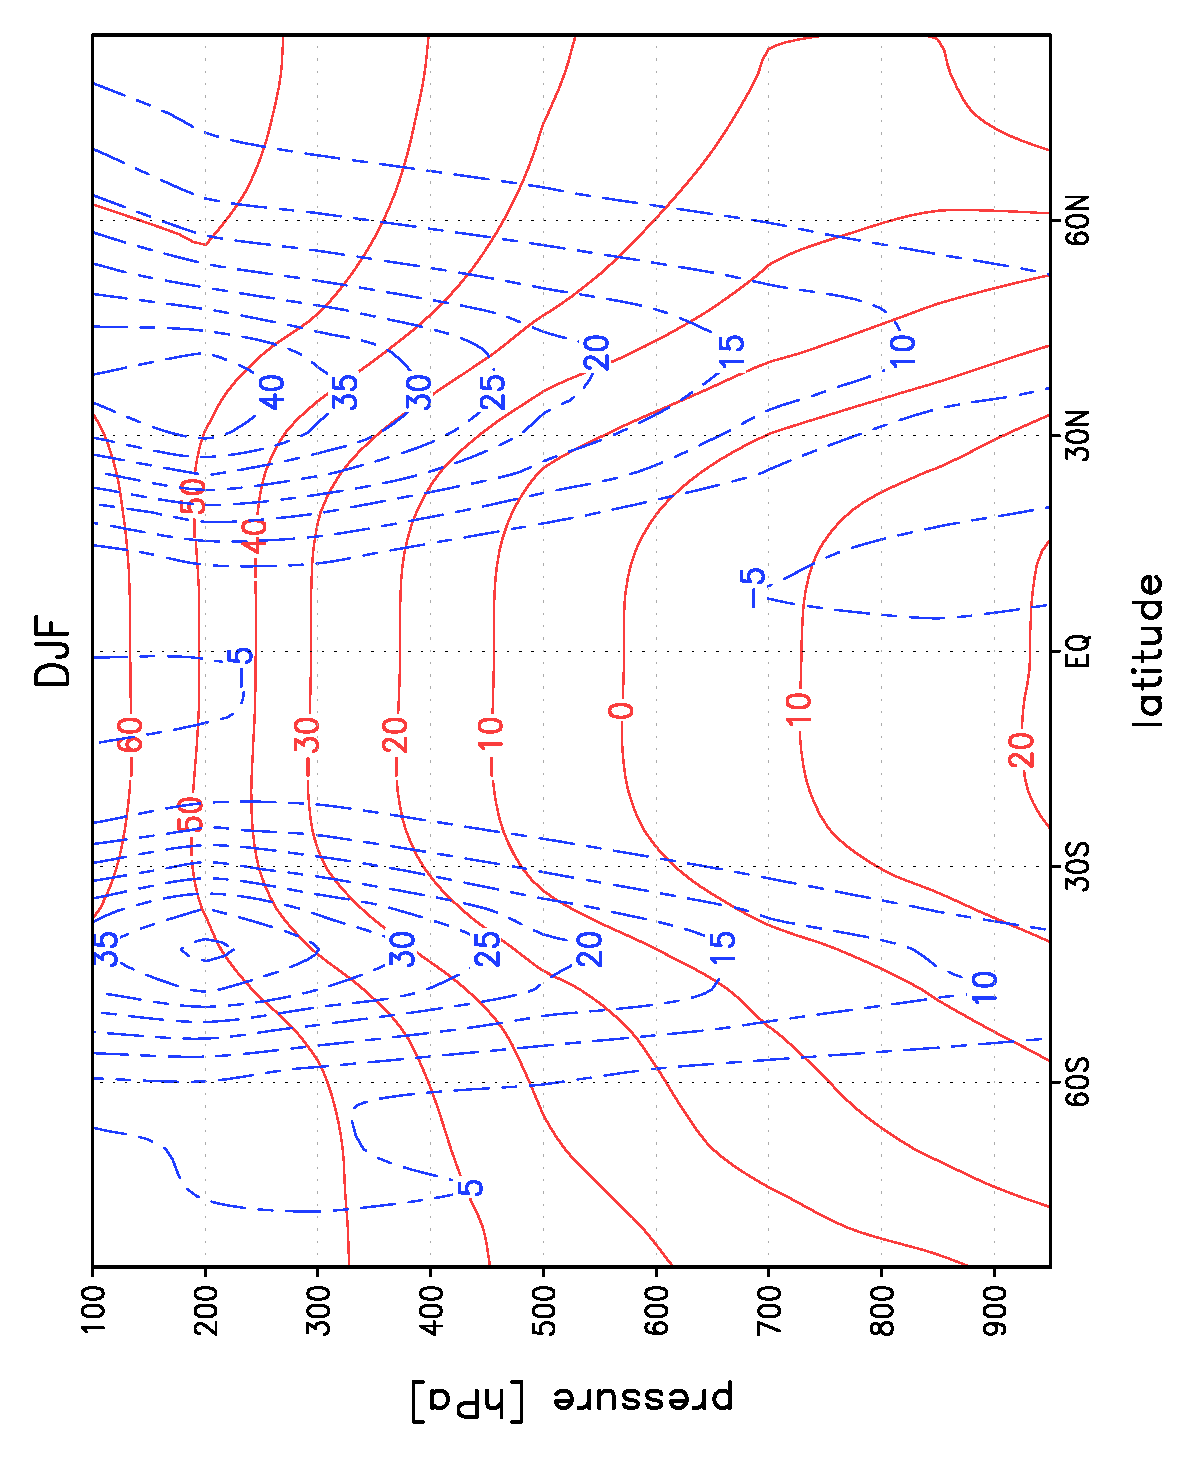
\includegraphics[height=8.5cm,width=6.5cm,angle=-90]
{eps/tempuallDJF.eps}
}
\parbox{8.5cm}{\hspace{1.05cm}\begin{scriptsize}(d)\end{scriptsize} \vspace{-0.5cm} \\
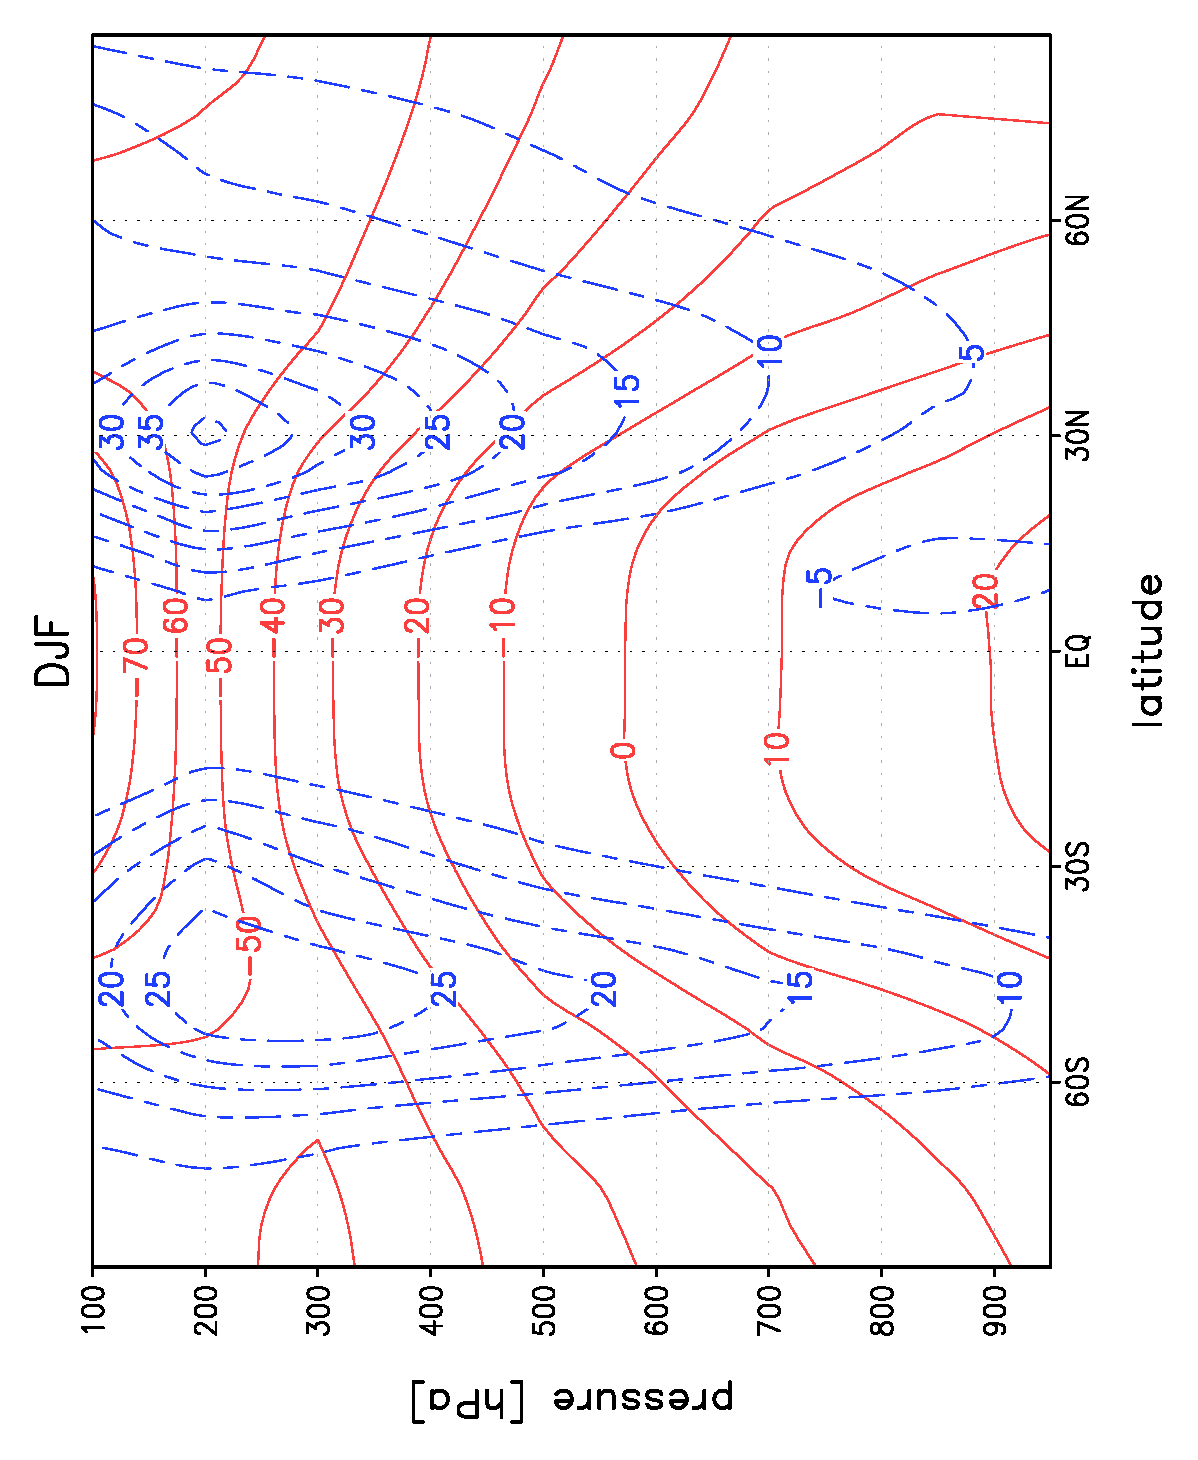
\includegraphics[height=8.5cm,width=6.5cm,angle=-90]
{eps/t21tempuallDJF.eps}
}
\parbox{8.5cm}{\hspace{1.00cm}\begin{scriptsize}(b)\end{scriptsize} \vspace{-0.5cm} \\
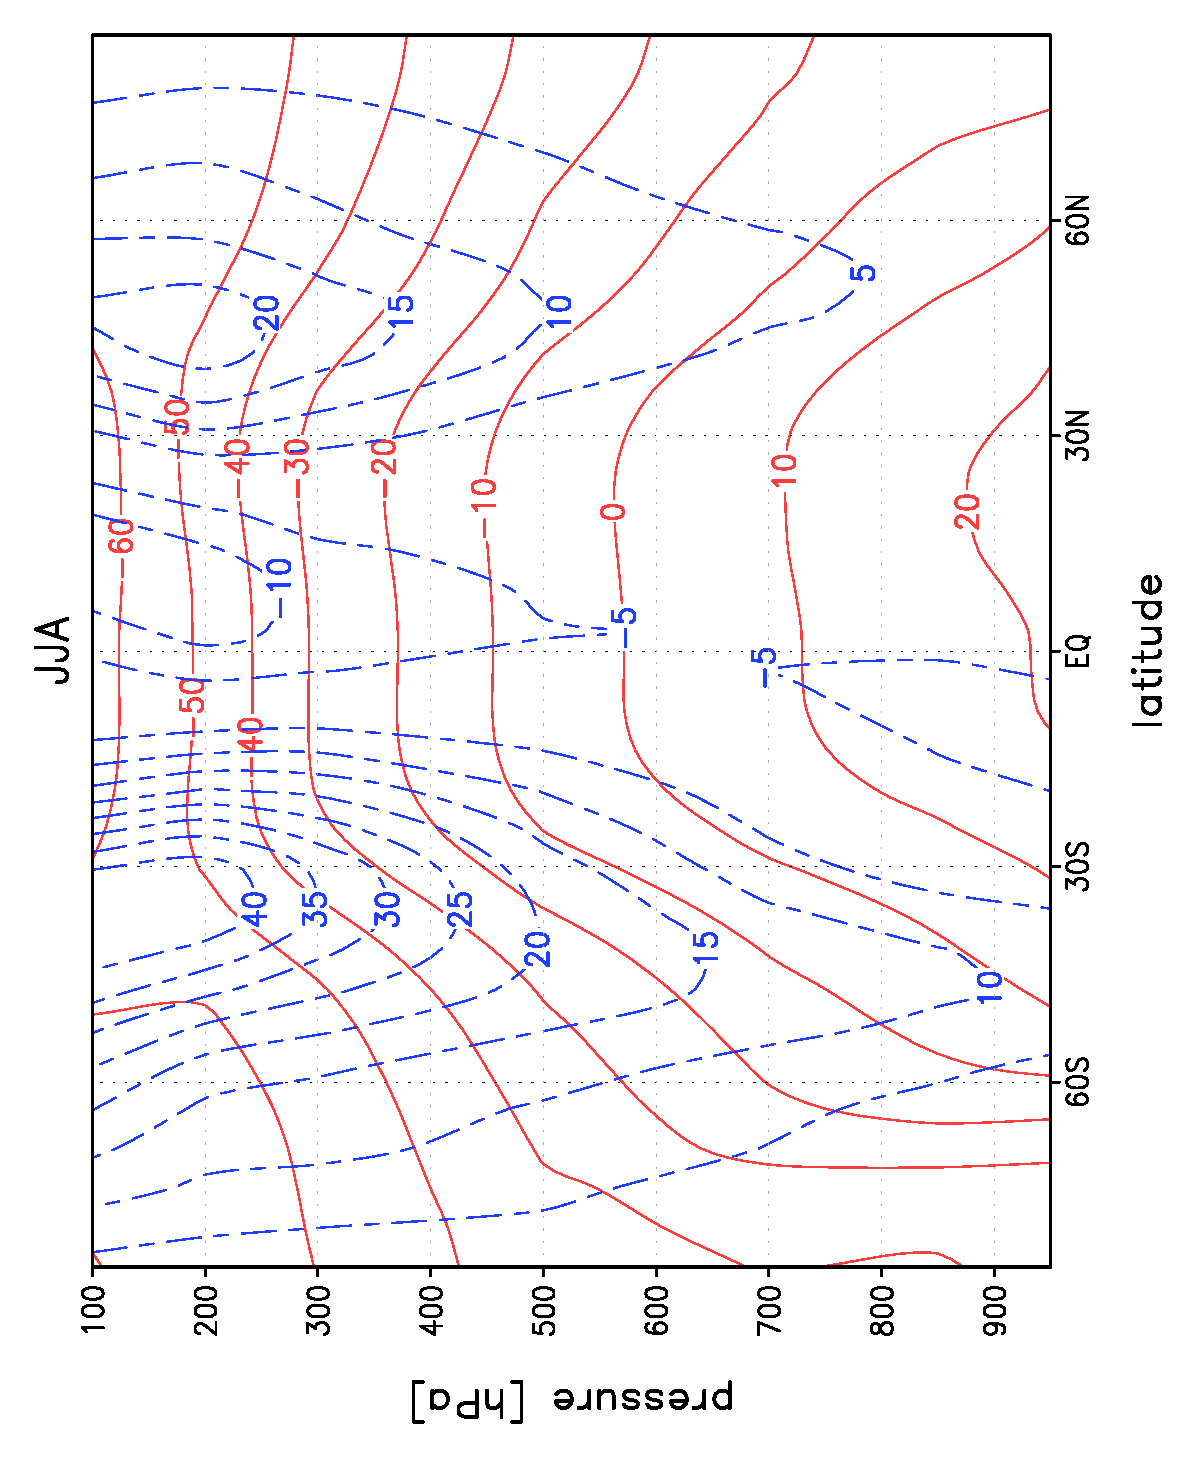
\includegraphics[height=8.5cm,width=6.5cm,angle=-90]
{eps/tempuallJJA.eps}
}
\parbox{8.5cm}{\hspace{1.05cm}\begin{scriptsize}(e)\end{scriptsize} \vspace{-0.5cm} \\
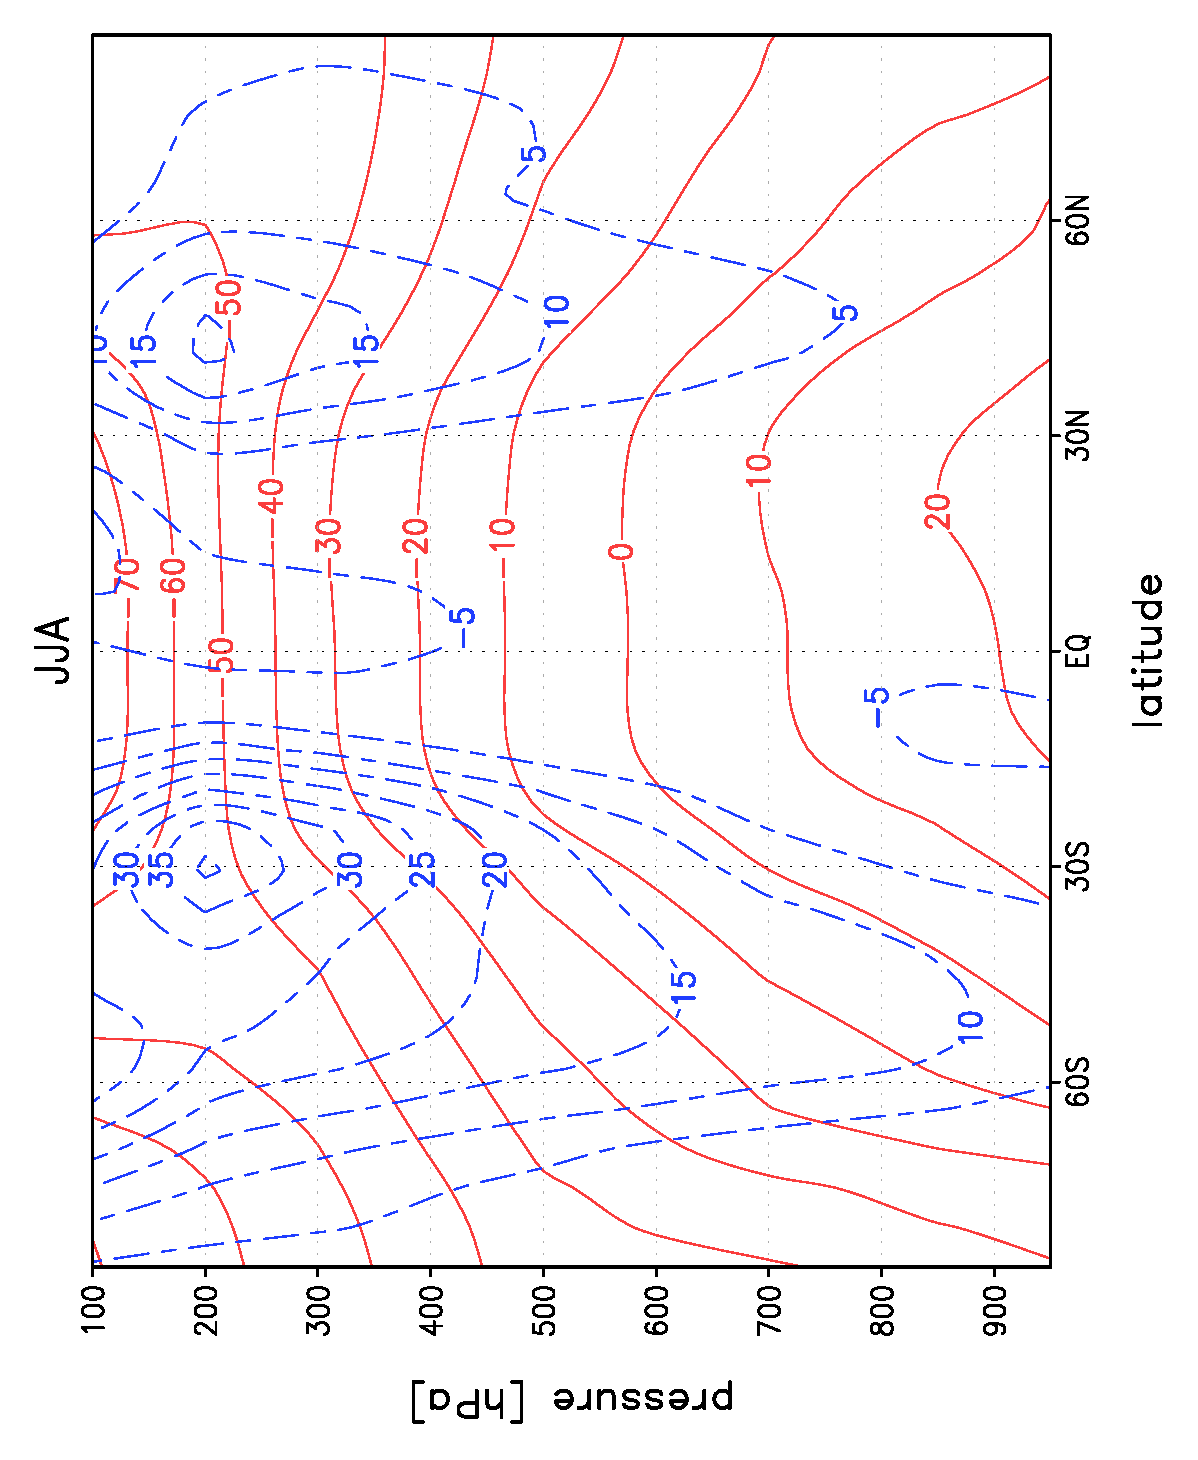
\includegraphics[height=8.5cm,width=6.5cm,angle=-90]
{eps/t21tempuallJJA.eps}
}
\parbox{8.5cm}{\hspace{1.00cm}\begin{scriptsize}(c)\end{scriptsize} \vspace{-0.5cm} \\
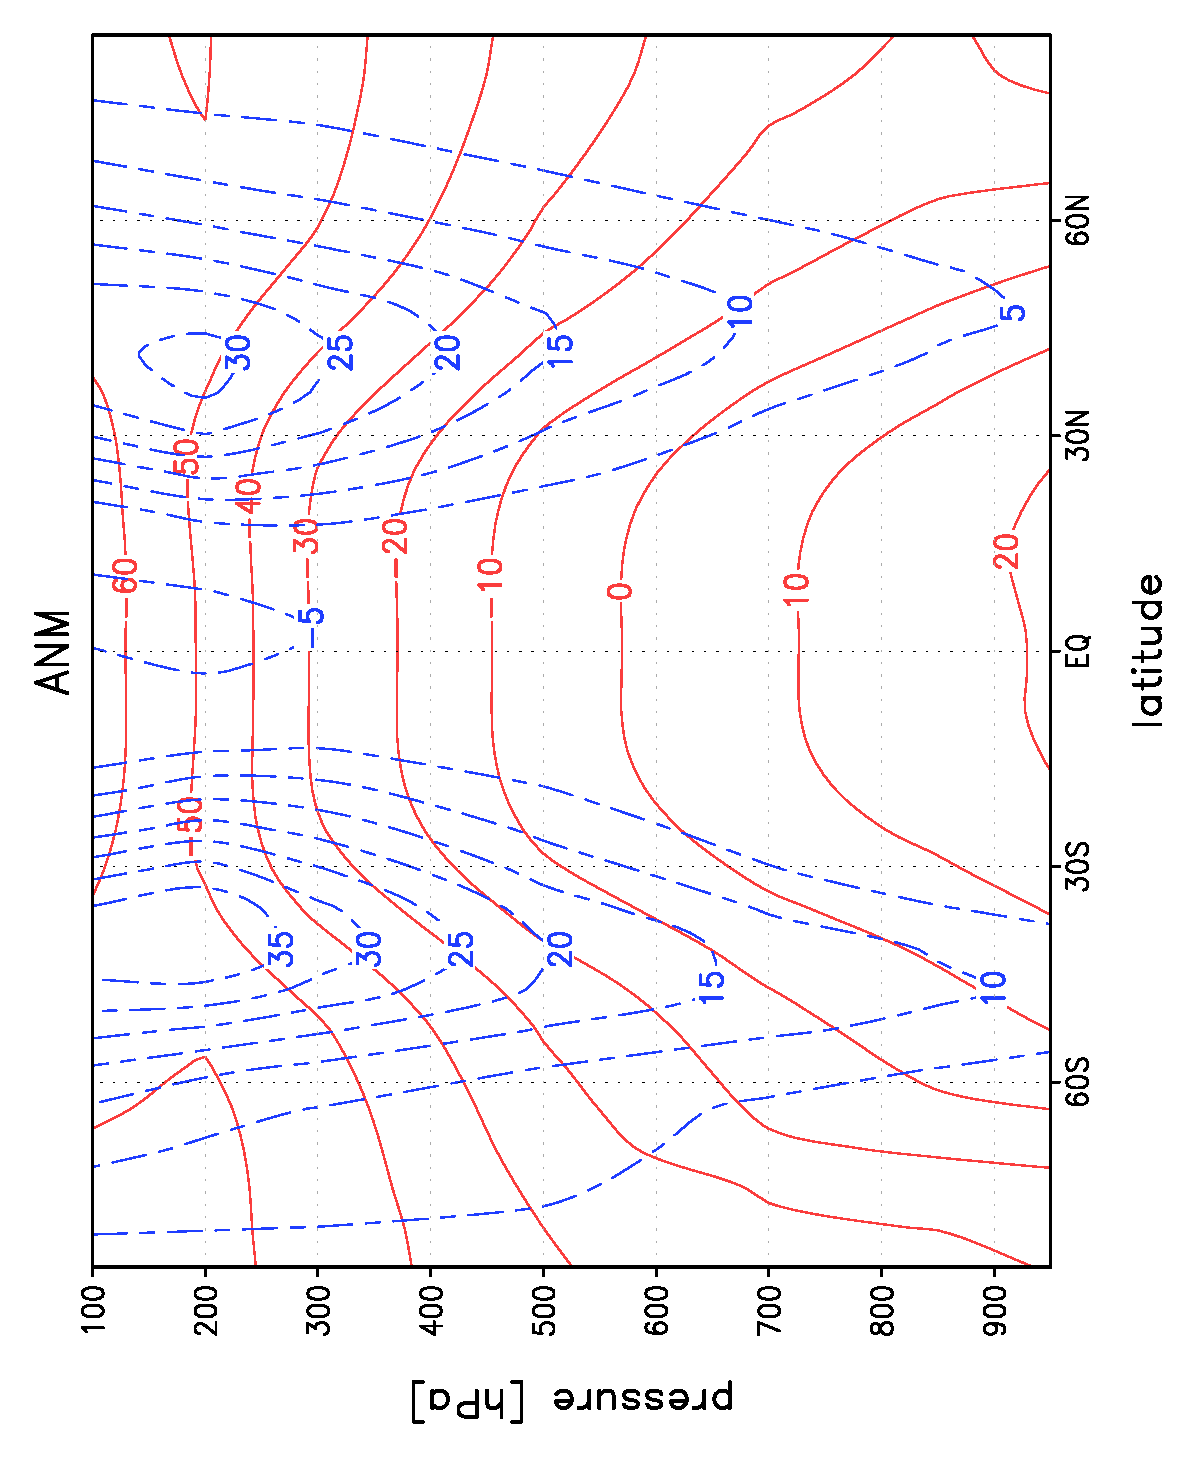
\includegraphics[height=8.5cm,width=6.5cm,angle=-90]
{eps/tmtempuall.eps}
}
\parbox{8.5cm}{\hspace{1.05cm}\begin{scriptsize}(f)\end{scriptsize} \vspace{-0.5cm} \\
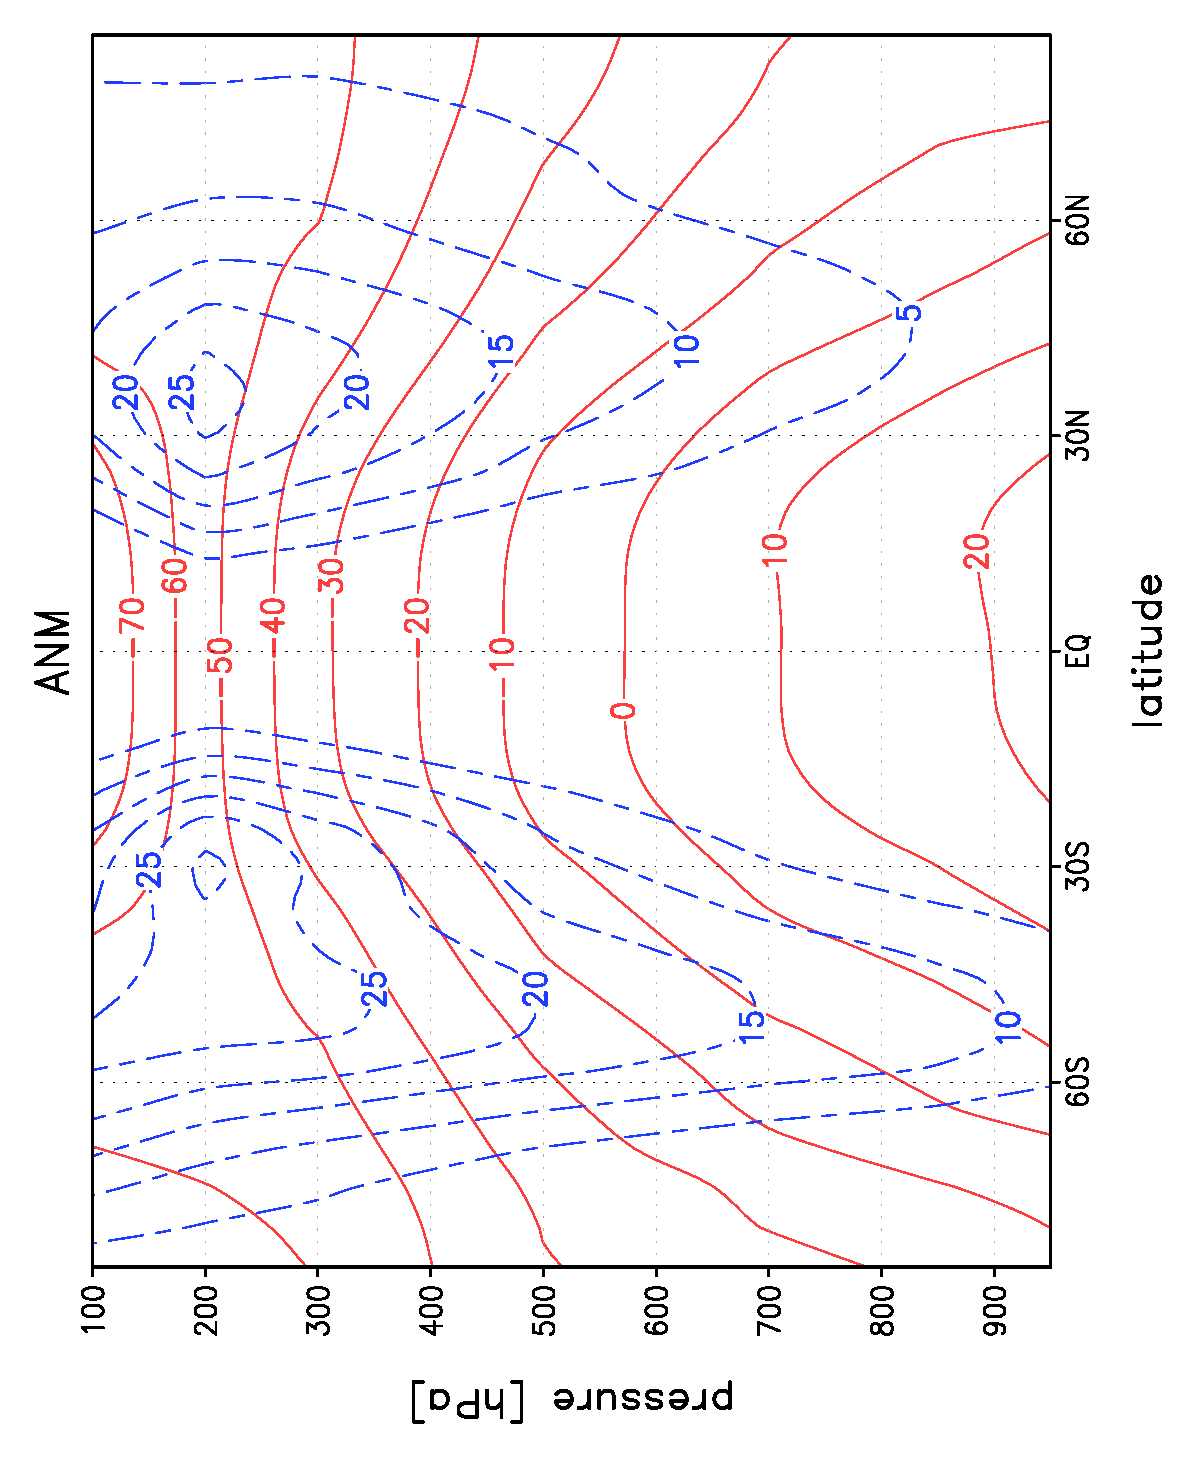
\includegraphics[height=8.5cm,width=6.5cm,angle=-90]
{eps/t21tmtempuall.eps}
}
\caption[Zonally averaged zonal wind and air temperature]{Zonally averaged zonal wind [m/s] and air temperature [°C]}
\label{img:tuall}
\end{figure}


\begin{figure}[H]
\hspace{4.1cm}PlaSim \hspace{7.4cm} ERA \\
\parbox{8.5cm}{\hspace{1.05cm}\begin{scriptsize}(a)\end{scriptsize} \vspace{-0.5cm} \\
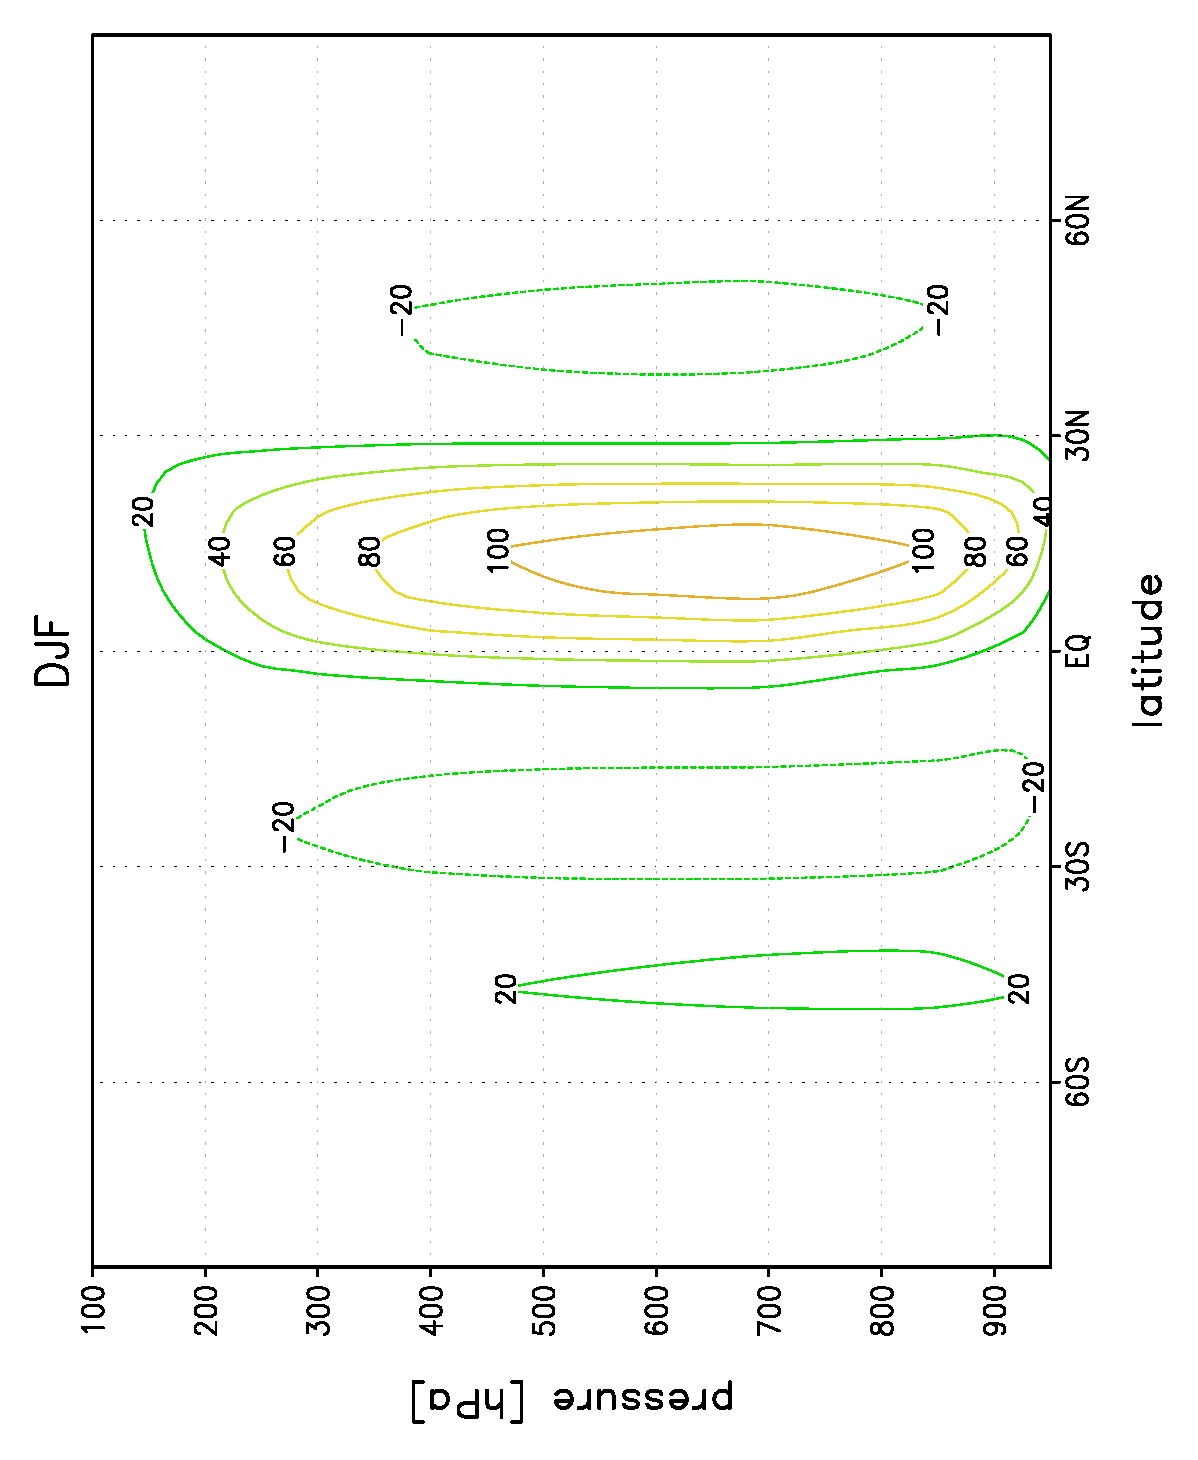
\includegraphics[height=8.5cm,width=6.5cm,angle=-90]
{eps/levelstreamDJF272.eps}
}
\parbox{8.5cm}{\hspace{1.05cm}\begin{scriptsize}(d)\end{scriptsize} \vspace{-0.5cm} \\
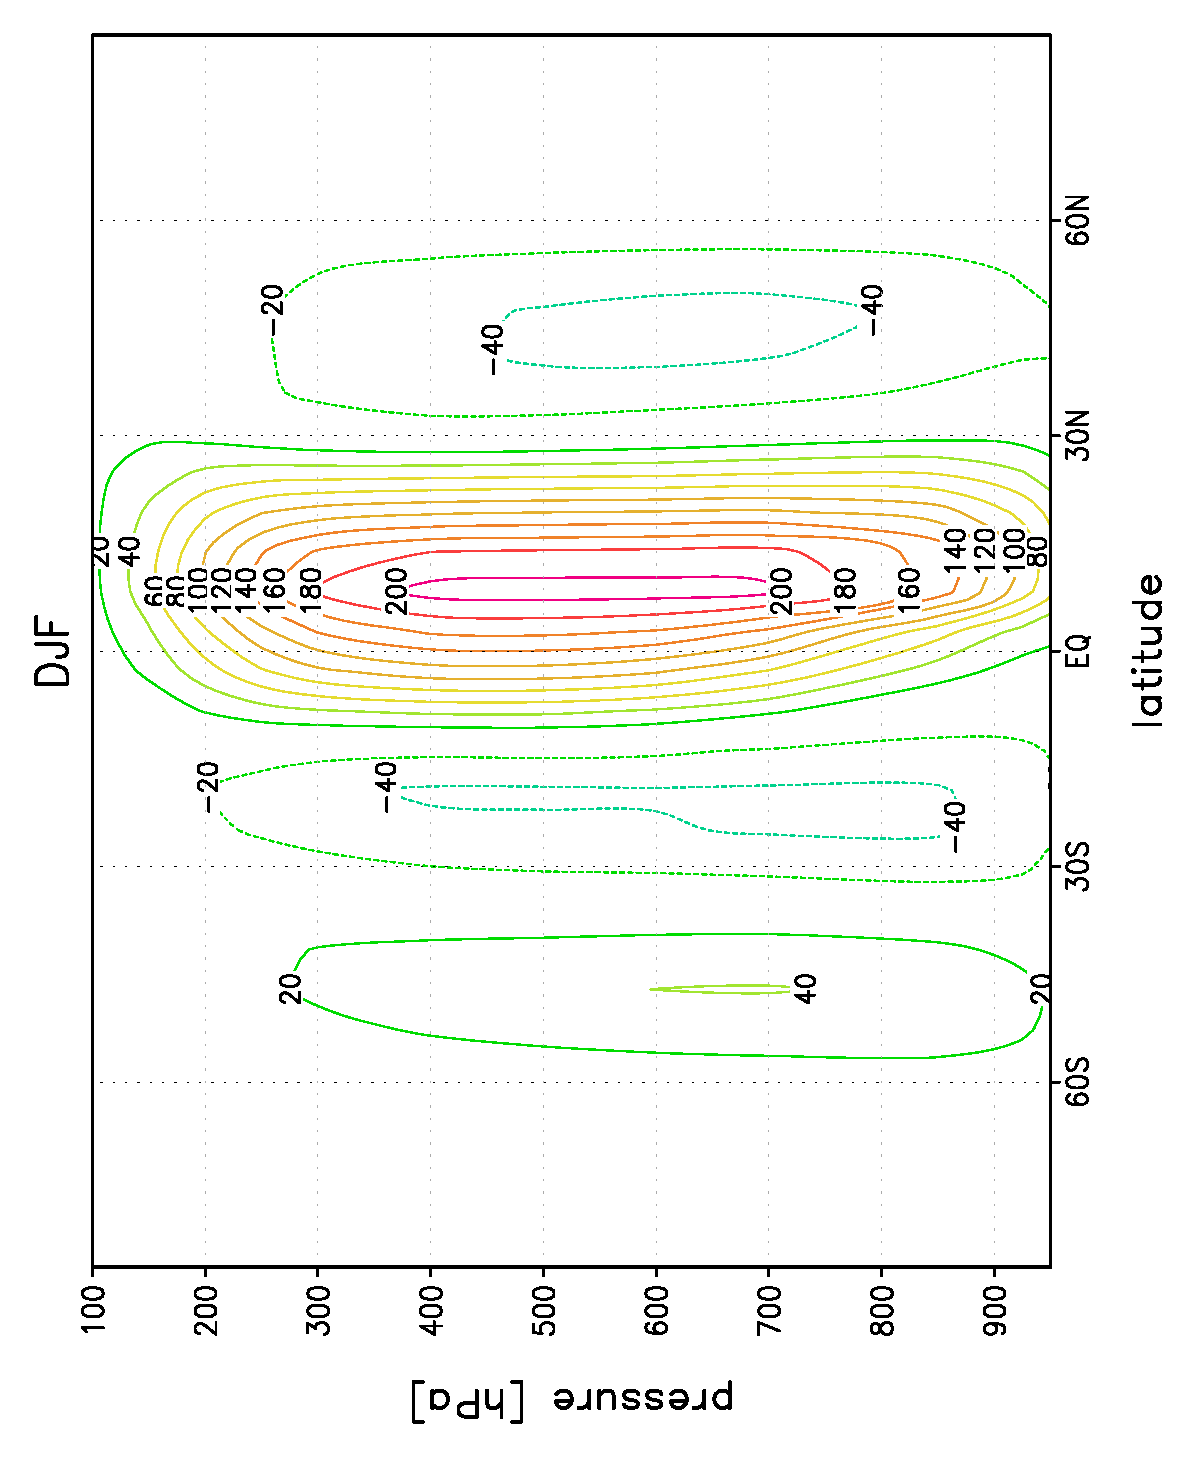
\includegraphics[height=8.5cm,width=6.5cm,angle=-90]
{eps/t21levelstreamDJF272.eps}
}
\parbox{8.5cm}{\hspace{1.05cm}\begin{scriptsize}(b)\end{scriptsize} \vspace{-0.5cm} \\
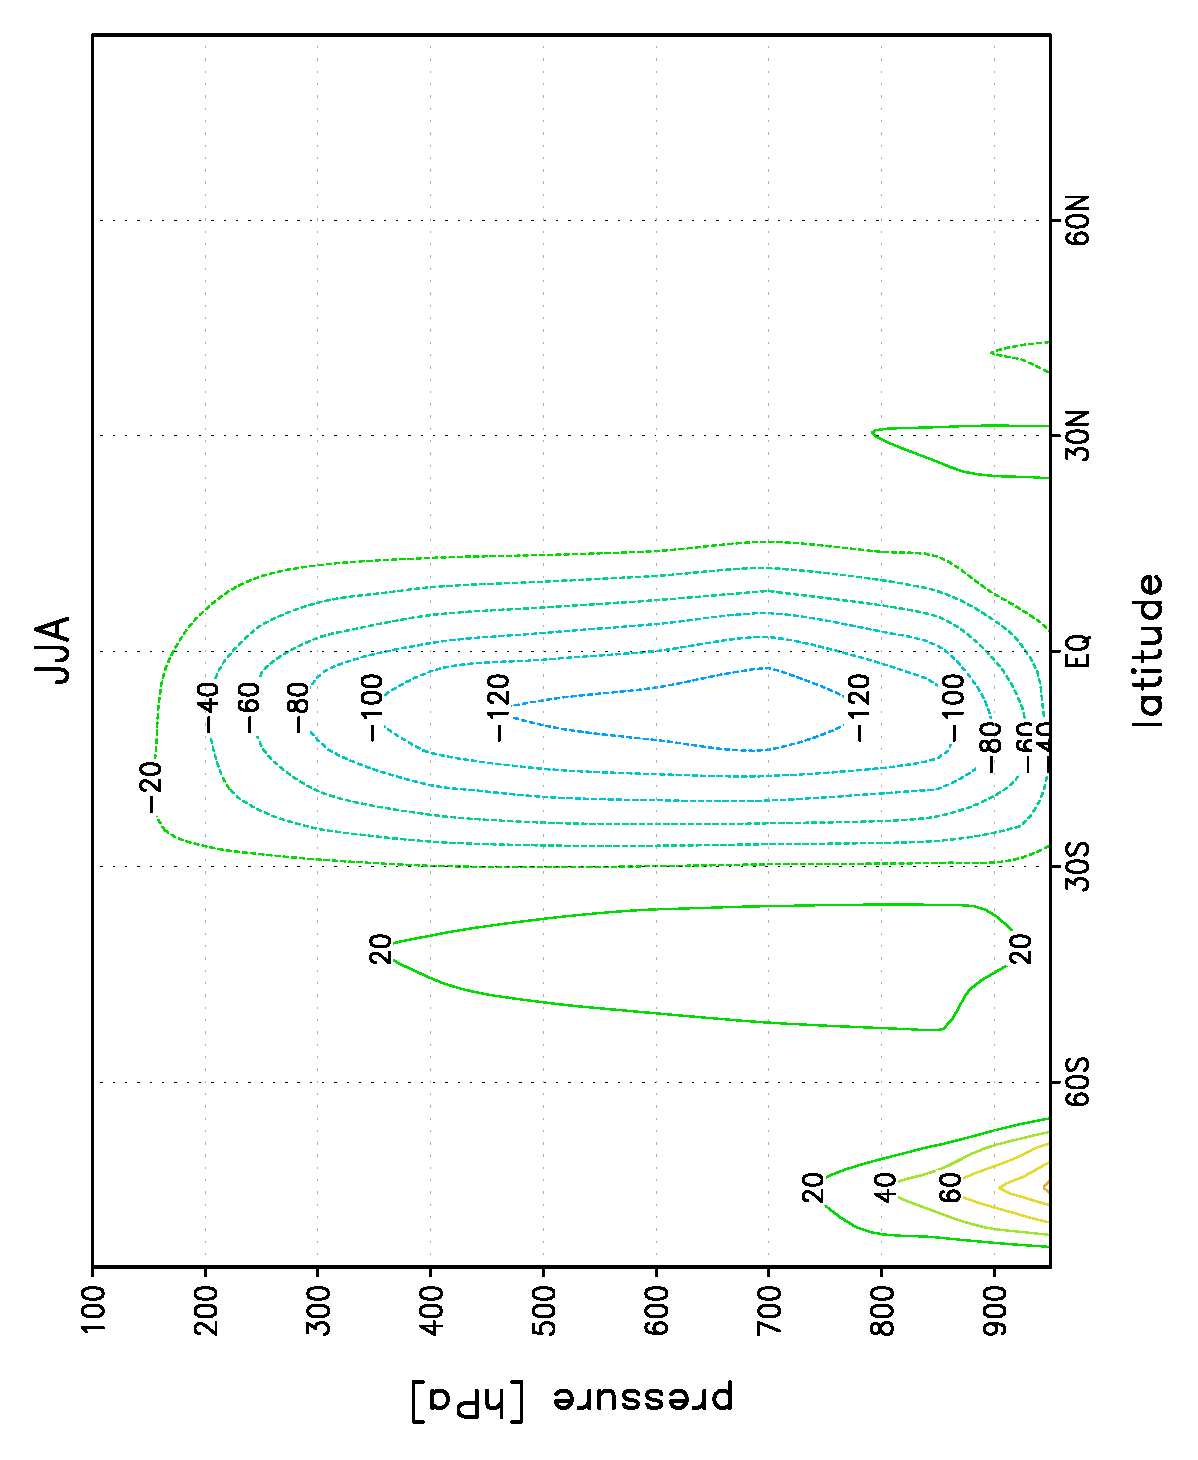
\includegraphics[height=8.5cm,width=6.5cm,angle=-90]
{eps/levelstreamJJA272.eps}
}
\parbox{8.5cm}{\hspace{1.05cm}\begin{scriptsize}(e)\end{scriptsize} \vspace{-0.5cm} \\
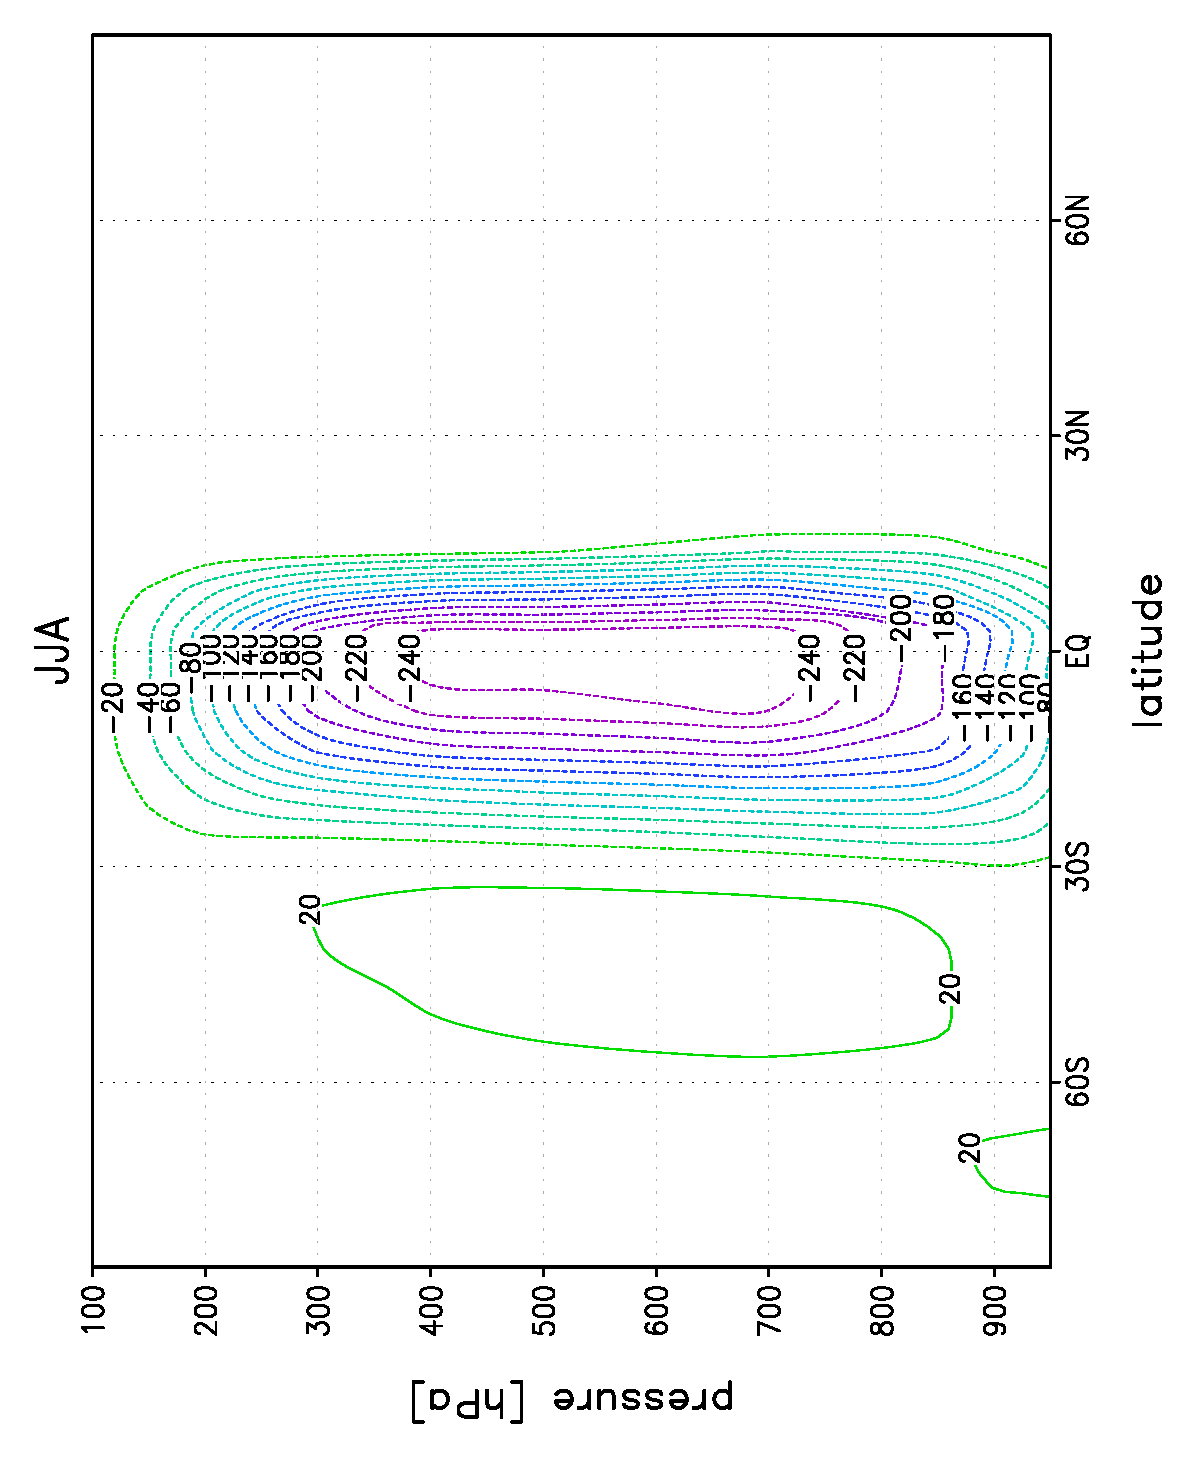
\includegraphics[height=8.5cm,width=6.5cm,angle=-90]
{eps/t21levelstreamJJA272.eps}
}
\parbox{8.5cm}{\hspace{1.05cm}\begin{scriptsize}(c)\end{scriptsize} \vspace{-0.5cm} \\
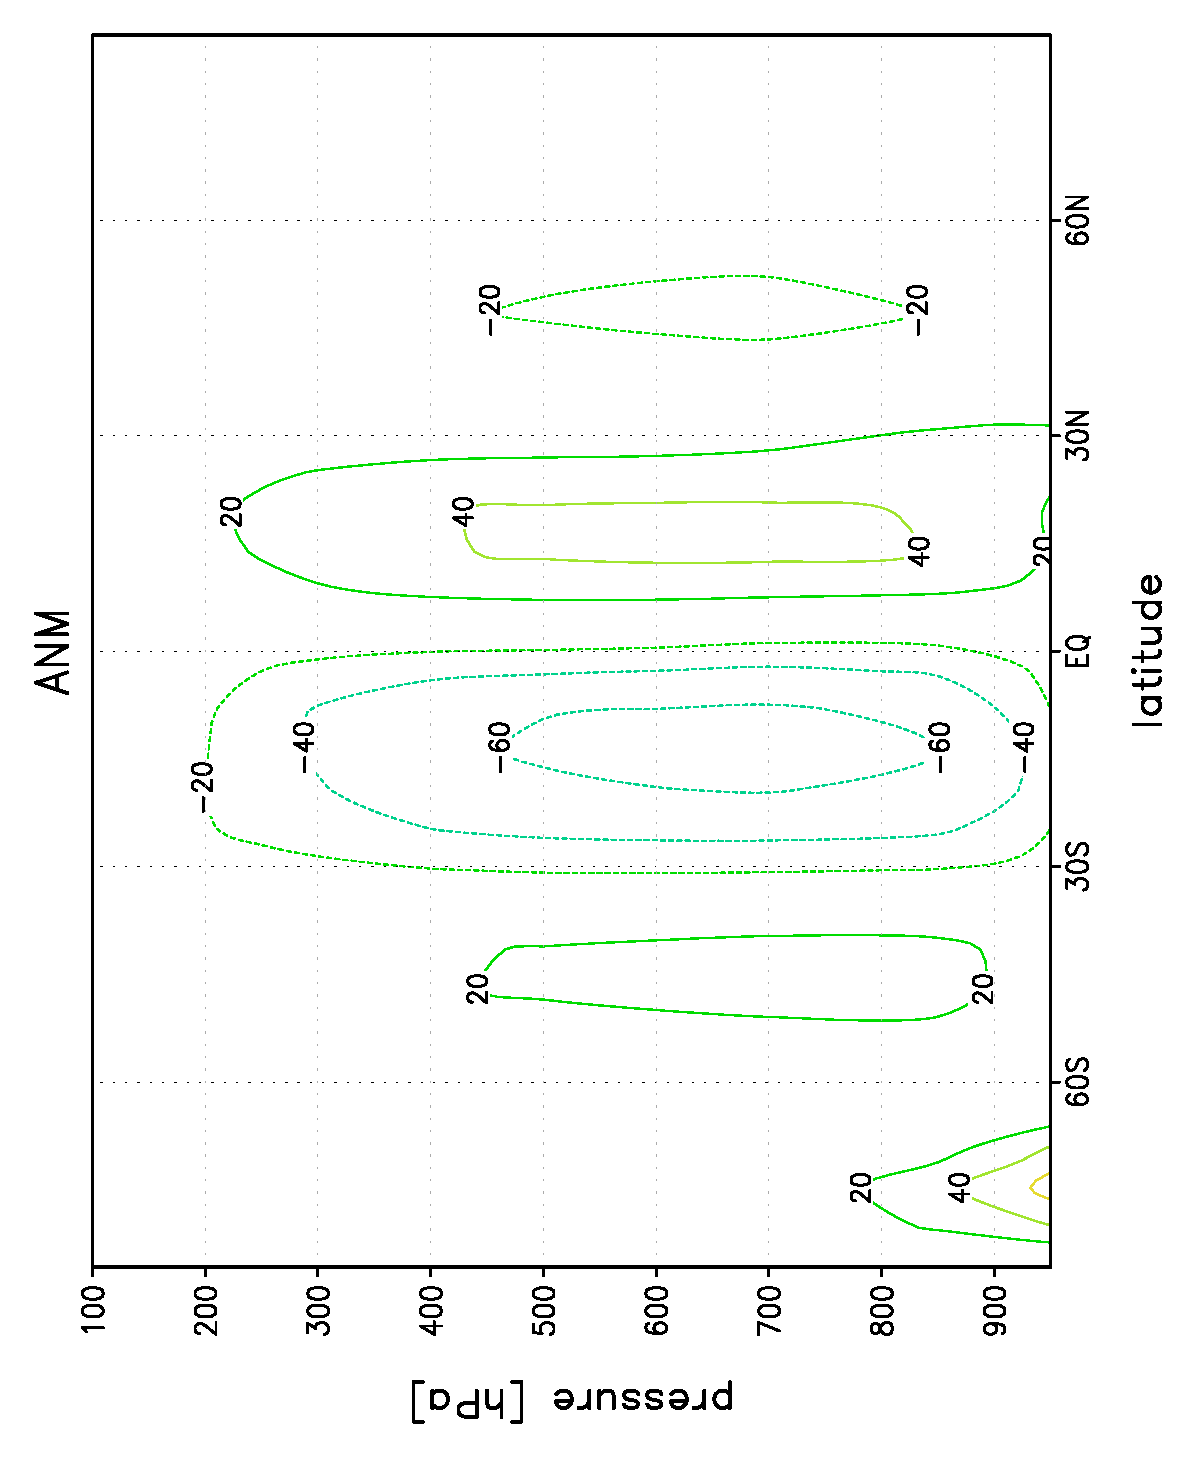
\includegraphics[height=8.5cm,width=6.5cm,angle=-90]
{eps/levelstreamANM272.eps}
}
\parbox{8.5cm}{\hspace{1.05cm}\begin{scriptsize}(f)\end{scriptsize} \vspace{-0.5cm} \\
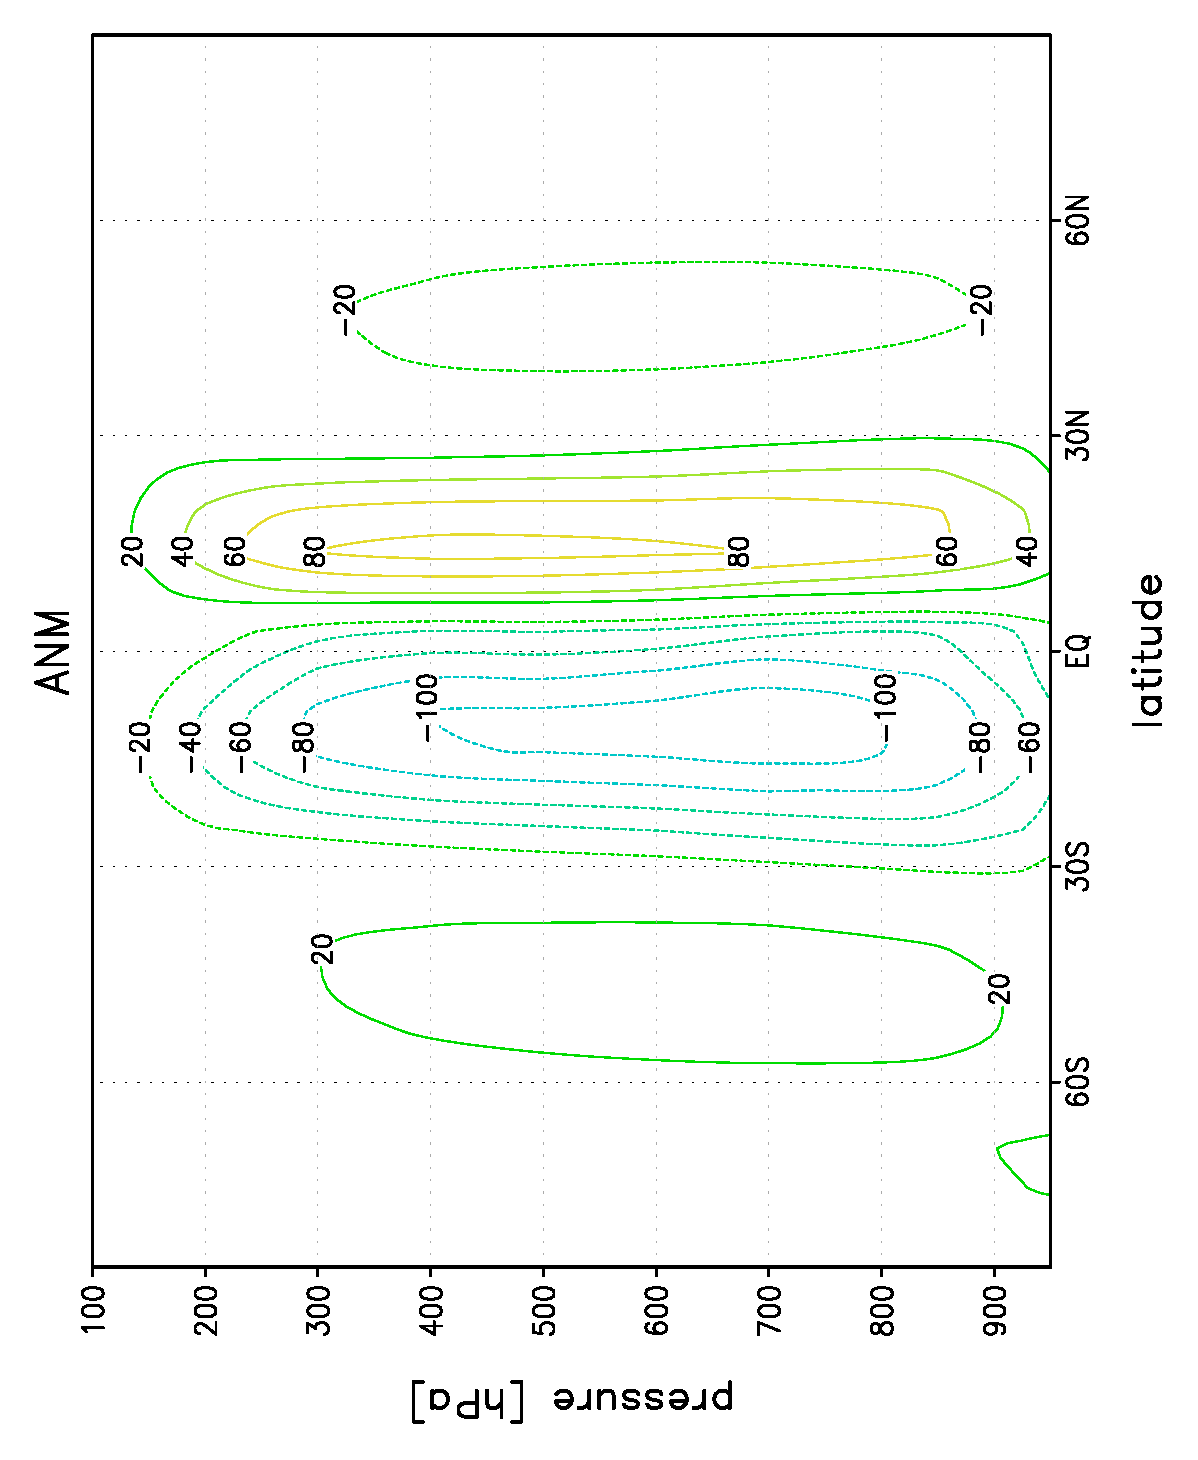
\includegraphics[height=8.5cm,width=6.5cm,angle=-90]
{eps/t21levelstreamANM272.eps}
}
\caption[Mass streamfunction]{Mass streamfunction $[10^{9}kg/s]$}
\label{img:streamfct}
\end{figure}


\vspace{-0.4cm}
\chapter{Global fields: temperature, pressure and winds}
\vspace{-0.4cm}

\section{Surface temperature}
\vspace{-0.4cm}

In NH winter, the temperature in the tropics ranges from 20 to 30° C, with a maximum > 30° C over Australia (Fig. \ref{img:surftemp} a, d). High NH summer temperatures (Fig. \ref{img:surftemp} b) above 30° C extend from Africa to Asia with PlaSim simulating another maximum over N-America, which does not appear in ERA (Fig. \ref{img:surftemp} e). The 2m-temperatures are similar but with reduced maxima (see Figures in appendix). In high latitudes, PlaSim implies a systematic cold bias in the respective winter hemisphere, which is attributed to the prescribed sea ice-distribution and also to the atmospheric humidity field affecting the radiative fluxes. The strongest PlaSim-ERA differences occur near the N-and S-Pole where minima are about -60° C and -80° C (compared to -40° C in ERA). This leads to lower global mean temperatures and affects the higher latitude dynamics. 


\vspace{-0.4cm}
\section{Mean sea level pressure}
\vspace{-0.4cm}


In NH winter (Fig. \ref{img:mslp} a, d), the mean sea level pressure shows the observed position and strength of Aleutian and Icelandic low in the mid-latitudes and of the equatorial trough. The subtropical highs are slightly overestimated and shifted northward (PlaSim: about 1022 hPa compared to 1018 hPa in ERA); the Azores High extends too far eastward. North of 60° N, PlaSim sea level pressure is higher (1020 hPa compared to 1015 hPa). The SH patterns are similar with larger magnitudes near the S-Pole.
At 60° S, PlaSim sea level pressure is about 10 hPa too high (998 hPa compared to 988 hPa in ERA). During NH summer (Fig. \ref{img:mslp} b, e), the deficiencies are similar, with the anticyclones in the N-Atlantic and N-Pacific being overestimated. The Asian Monsoon low extends to South East Asia where it is slightly too weak in PlaSim indicative of an underestimated Indian Summer Monsoon. The zonal profile demonstrates the differences between PlaSim and ERA in the SH. The subtropical high is shifted poleward and the mid-latitude low pressure belt near 60° S is too weak (1000 hPa compared to 988 hPa in ERA). South of 60° S, the structures are very different. Over the S-Pole, PlaSim simulates lower pressure of 998 hPa compared to 1005 hPa in ERA.


\begin{figure}[H]
\hspace{3.0cm}PlaSim \vspace{0.2cm} \hspace{7.2cm} ERA \\
\parbox{8.5cm}{\hspace{0.50cm}\begin{scriptsize}(a)\end{scriptsize} \vspace{-0.7cm} \\
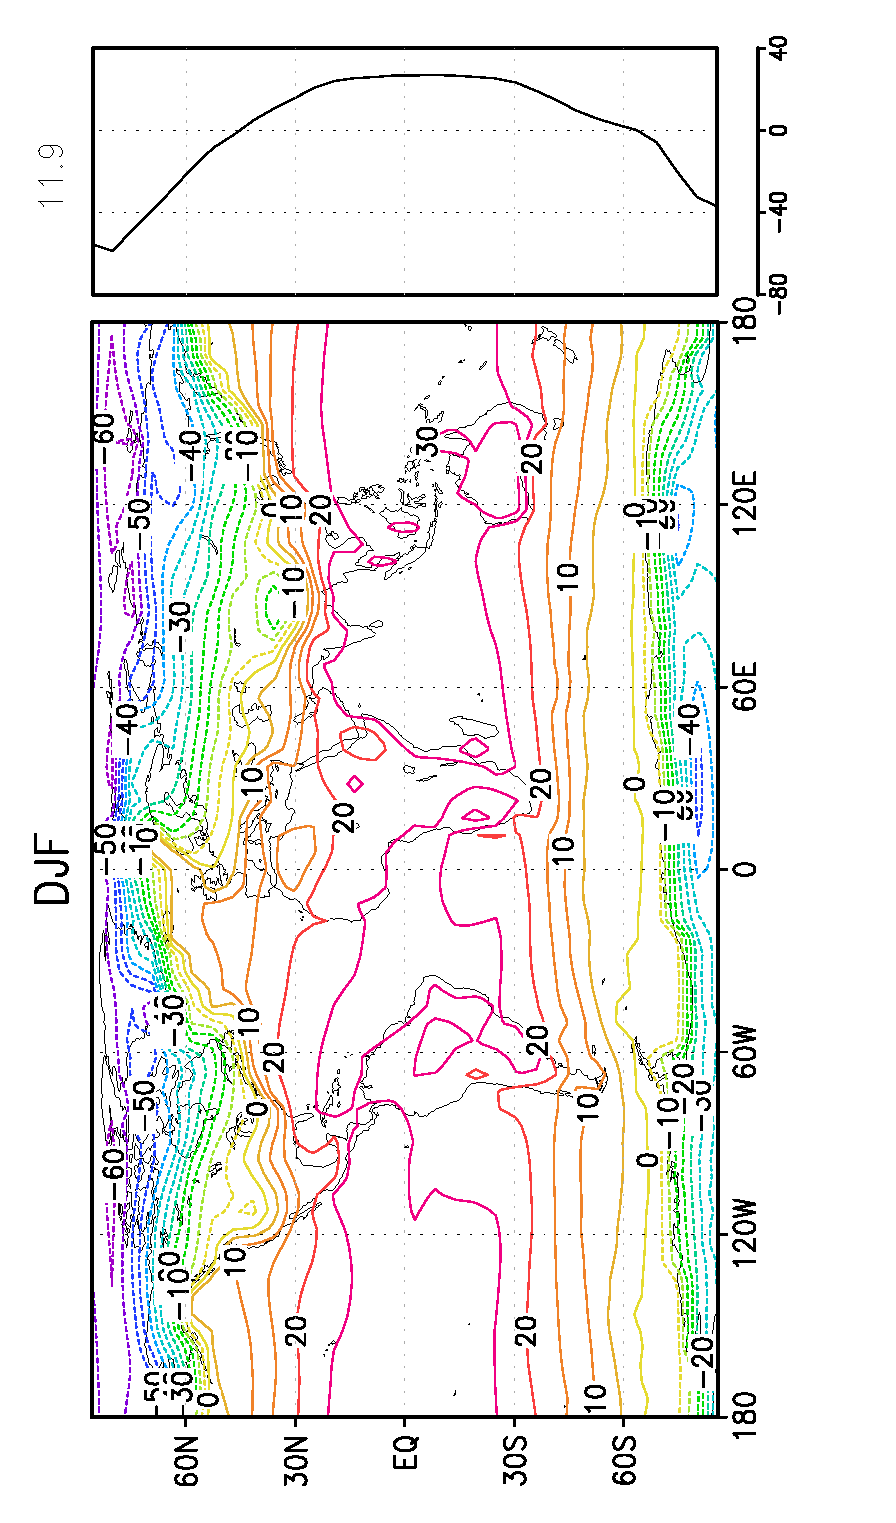
\includegraphics[height=8.5cm,width=6.5cm,angle=-90]
{eps/zonalcelysmtemp139DJF.eps}
}
\parbox{8.5cm}{\hspace{0.25cm}\begin{scriptsize}(d)\end{scriptsize} \vspace{-0.7cm} \\
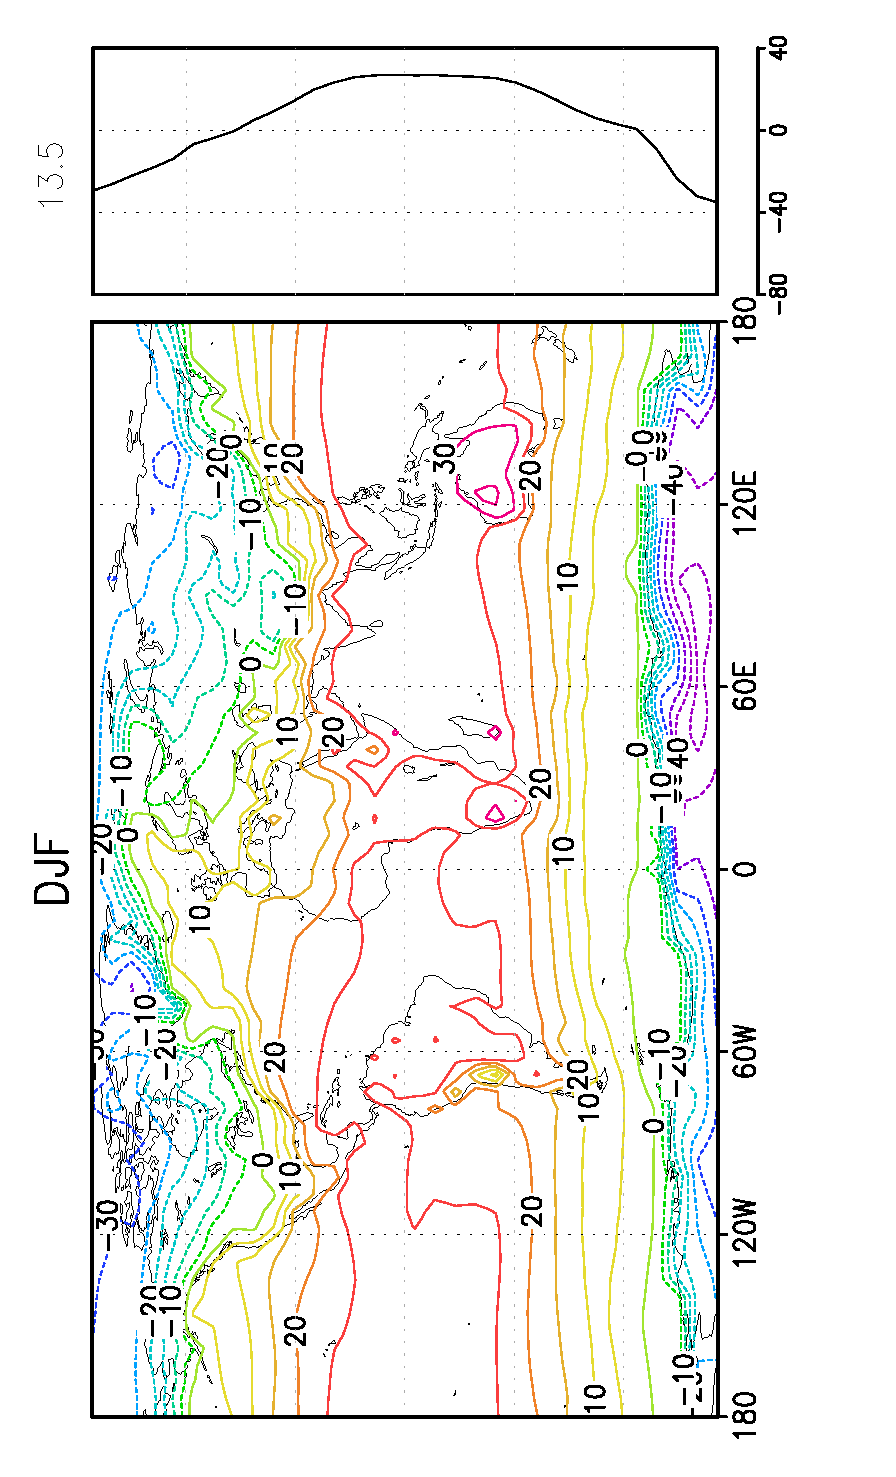
\includegraphics[height=8.5cm,width=6.5cm,angle=-90]
{eps/zonalt21celysmsoil139DJF.eps}
}
\parbox{8.5cm}{\hspace{0.50cm}\begin{scriptsize}(b)\end{scriptsize} \vspace{-0.7cm} \\
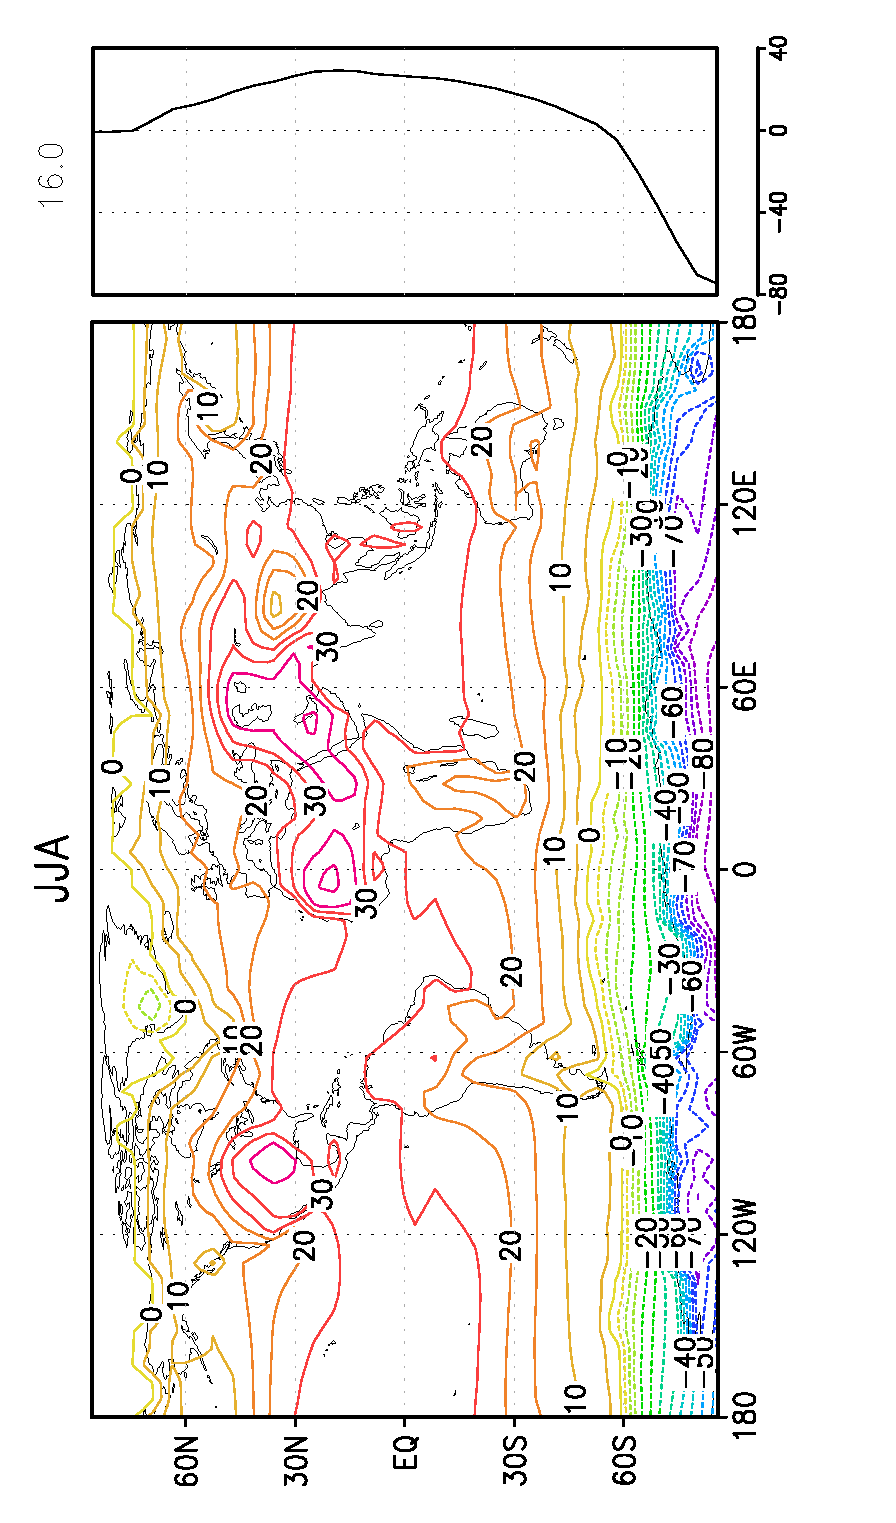
\includegraphics[height=8.5cm,width=6.5cm,angle=-90]
{eps/zonalcelysmtemp139JJA.eps}
}
\parbox{8.5cm}{\hspace{0.25cm}\begin{scriptsize}(e)\end{scriptsize} \vspace{-0.7cm} \\
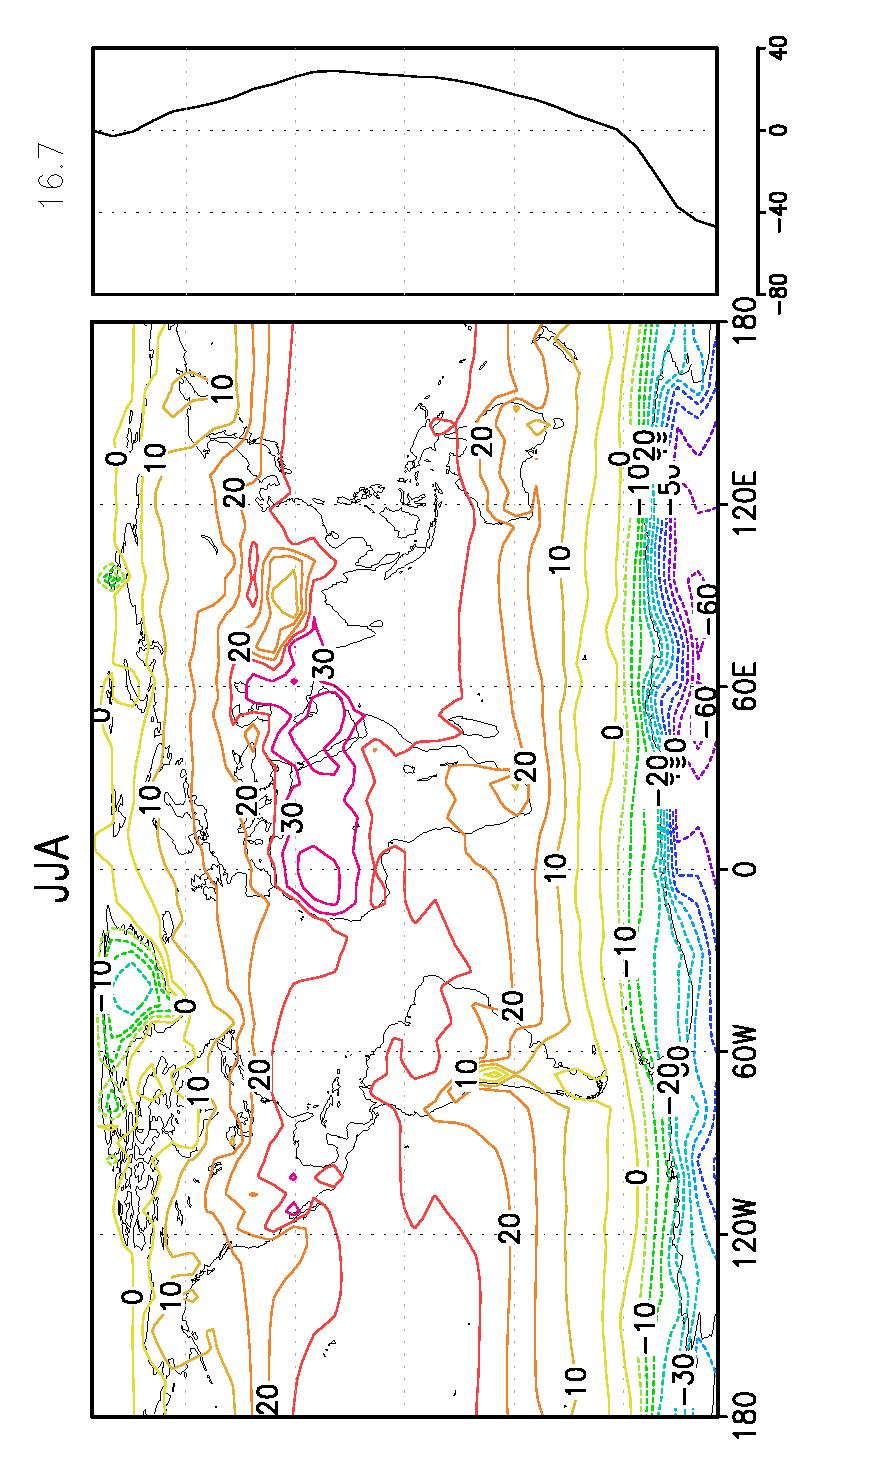
\includegraphics[height=8.5cm,width=6.5cm,angle=-90]
{eps/zonalt21celysmsoil139JJA.eps}
}
\parbox{8.5cm}{\hspace{0.50cm}\begin{scriptsize}(c)\end{scriptsize} \vspace{-0.7cm} \\
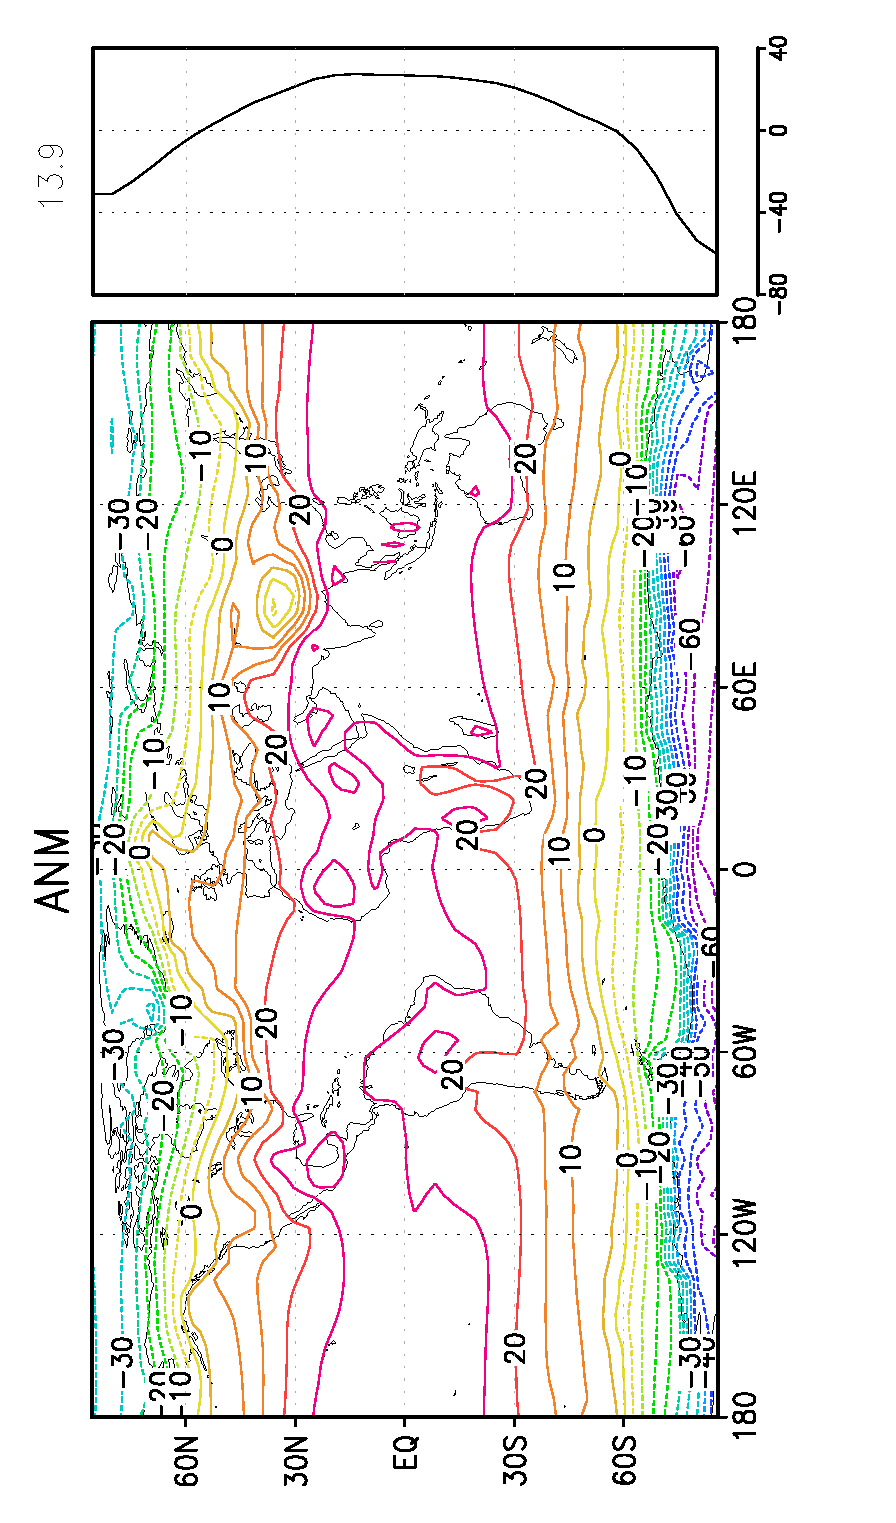
\includegraphics[height=8.5cm,width=6.5cm,angle=-90]
{eps/zonalceltmtemp139.eps}
}
\parbox{8.5cm}{\hspace{0.25cm}\begin{scriptsize}(f)\end{scriptsize} \vspace{-0.7cm} \\
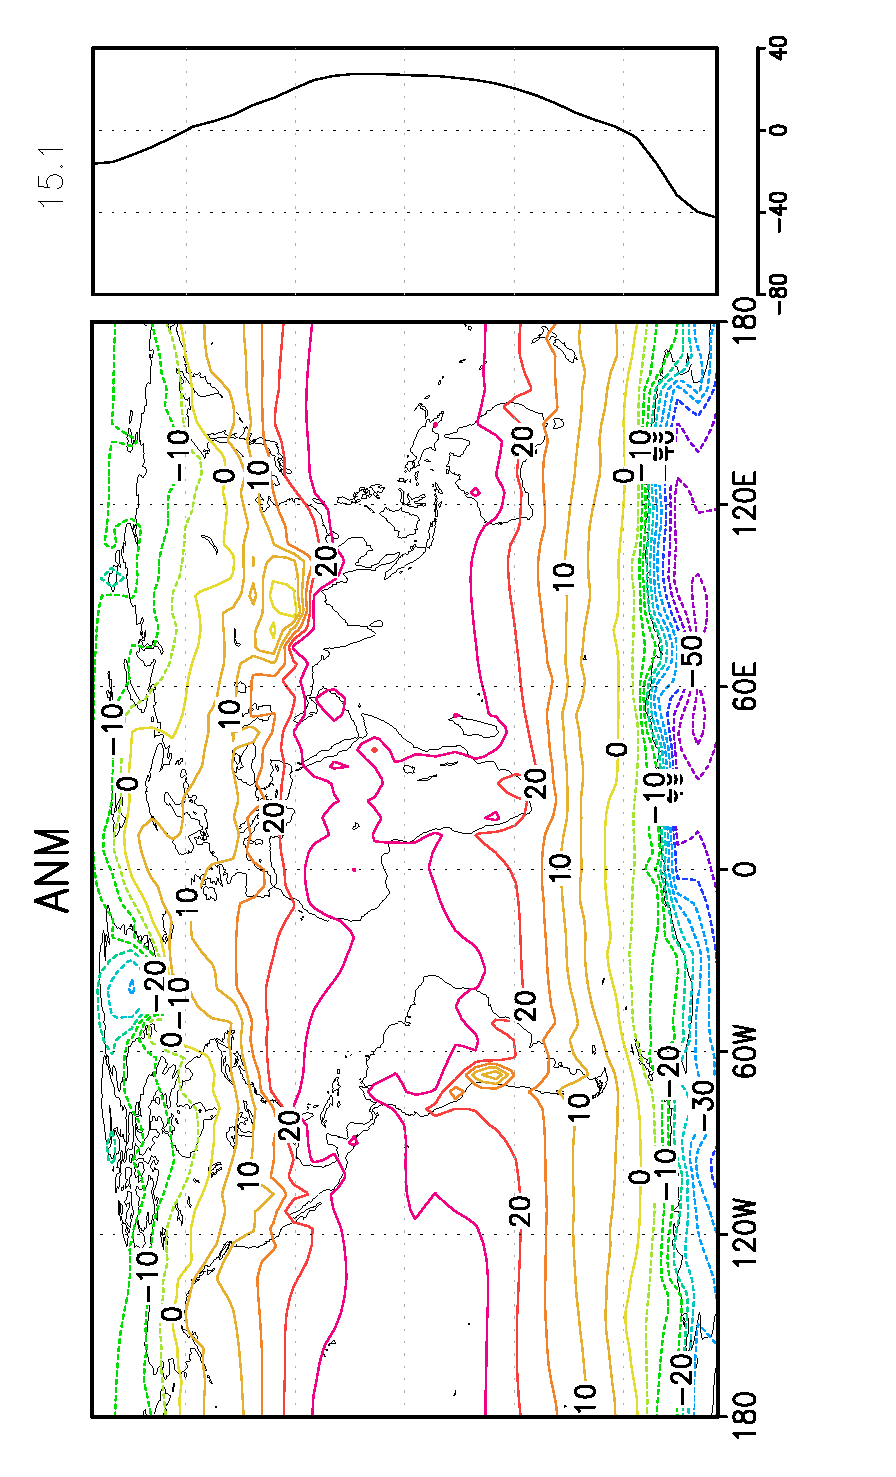
\includegraphics[height=8.5cm,width=6.5cm,angle=-90]
{eps/zonalt21celtmsoil.eps}
}
\caption[Surface temperature]{Surface temperature [°C]; right panels: zonal mean with global mean on top}
\label{img:surftemp}
\end{figure}


\begin{figure}[H]
\hspace{3.0cm}PlaSim \vspace{0.1cm}\hspace{7.2cm} ERA \\
\parbox{8.5cm}{\hspace{0.50cm}\begin{scriptsize}(a)\end{scriptsize} \vspace{-0.7cm} \\
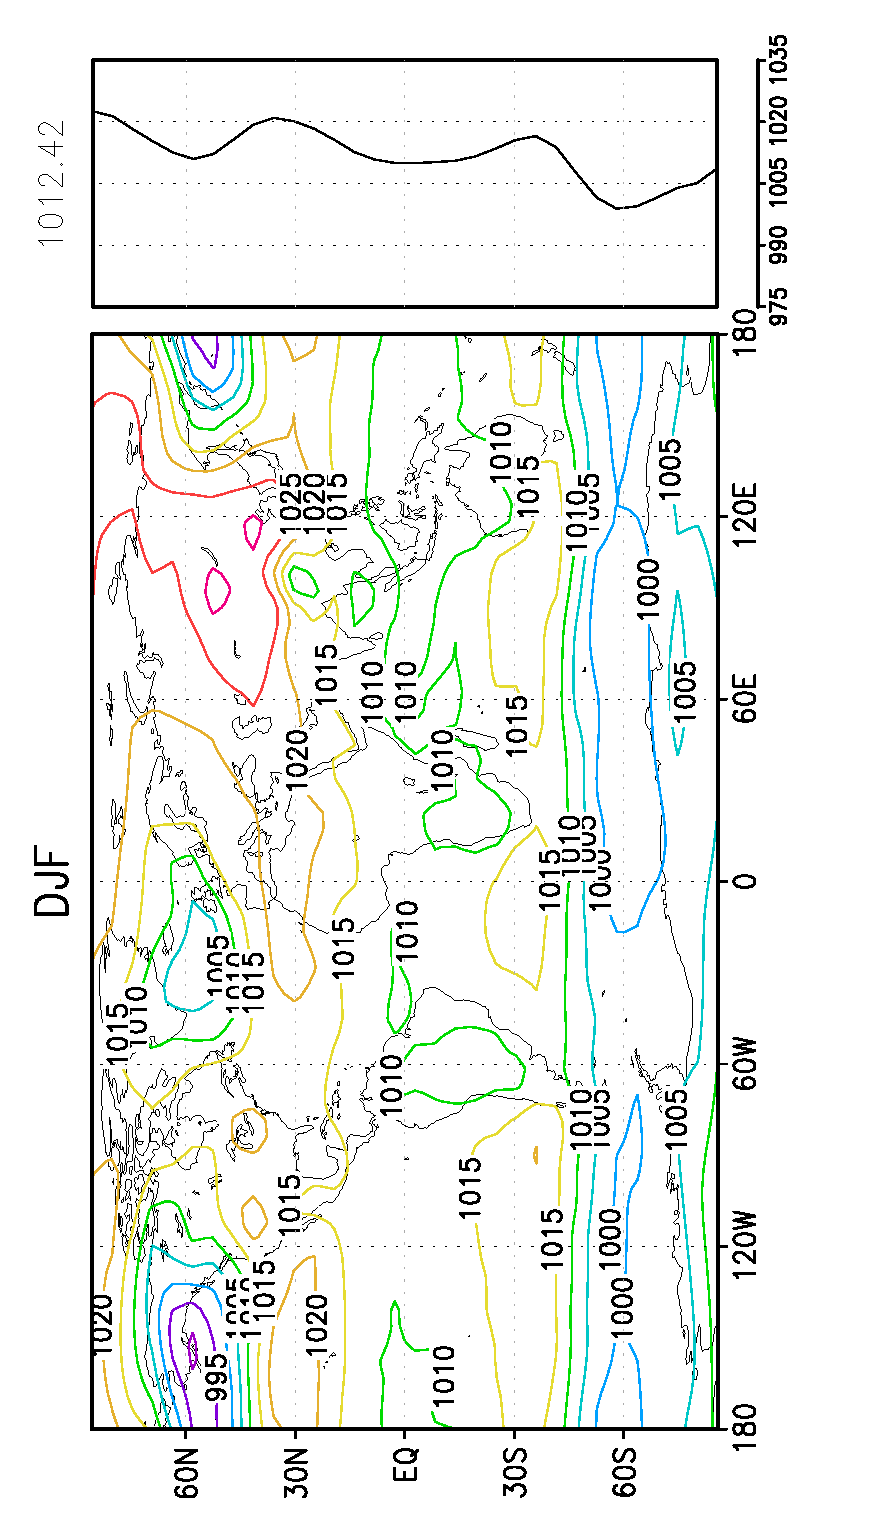
\includegraphics[height=8.5cm,width=6.5cm,angle=-90]
{eps/zonalfinalysmpres151DJF.eps}
}
\parbox{8.5cm}{\hspace{0.25cm}\begin{scriptsize}(d)\end{scriptsize} \vspace{-0.7cm} \\
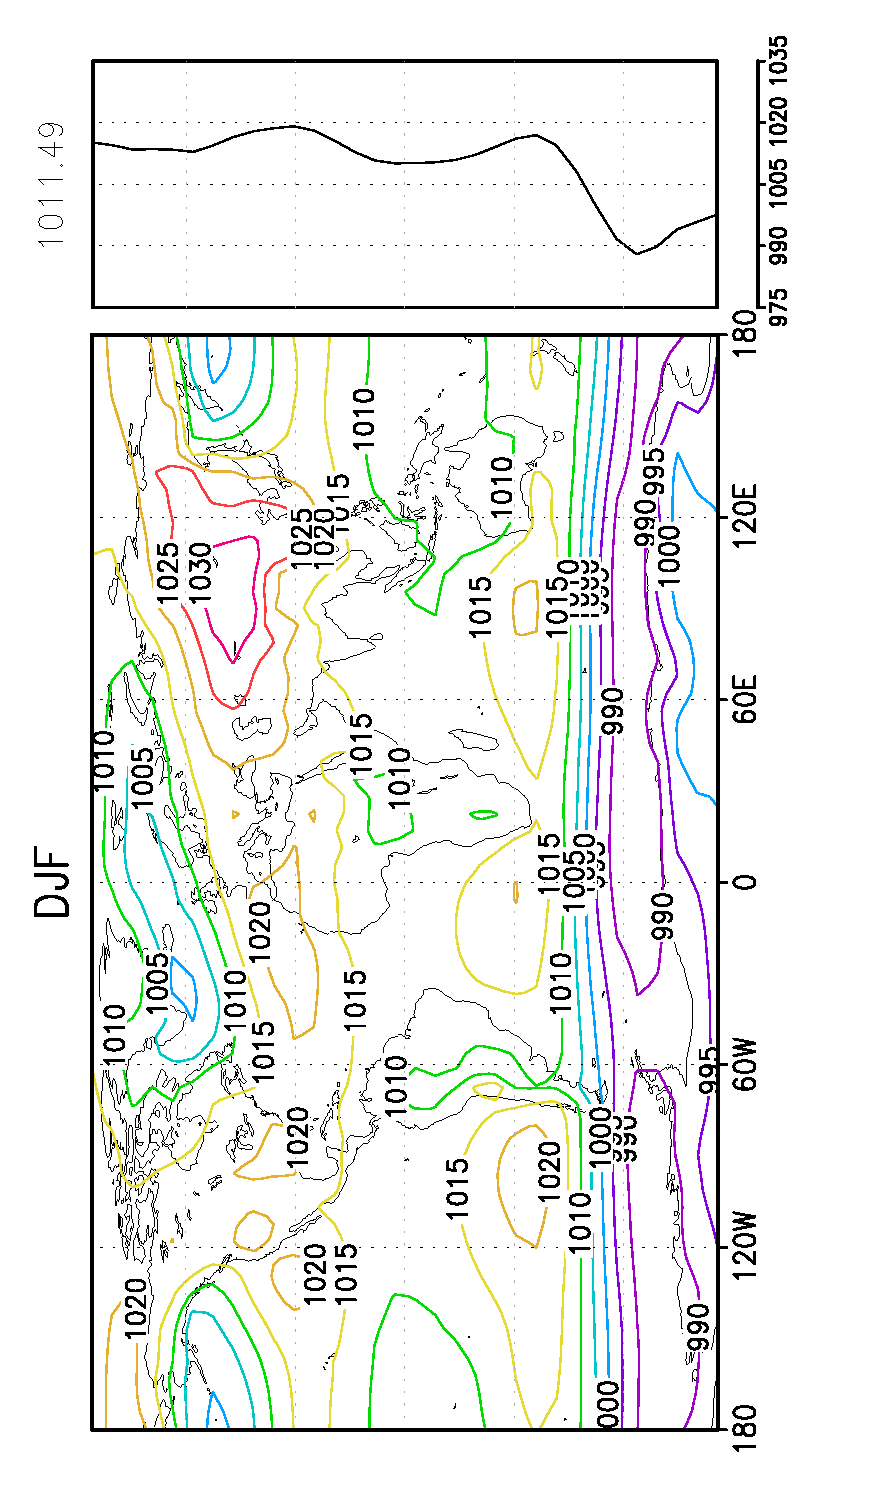
\includegraphics[height=8.5cm,width=6.5cm,angle=-90]
{eps/zonalt21finalysmmslpDJF.eps}
}
\parbox{8.5cm}{\hspace{0.50cm}\begin{scriptsize}(b)\end{scriptsize} \vspace{-0.7cm} \\
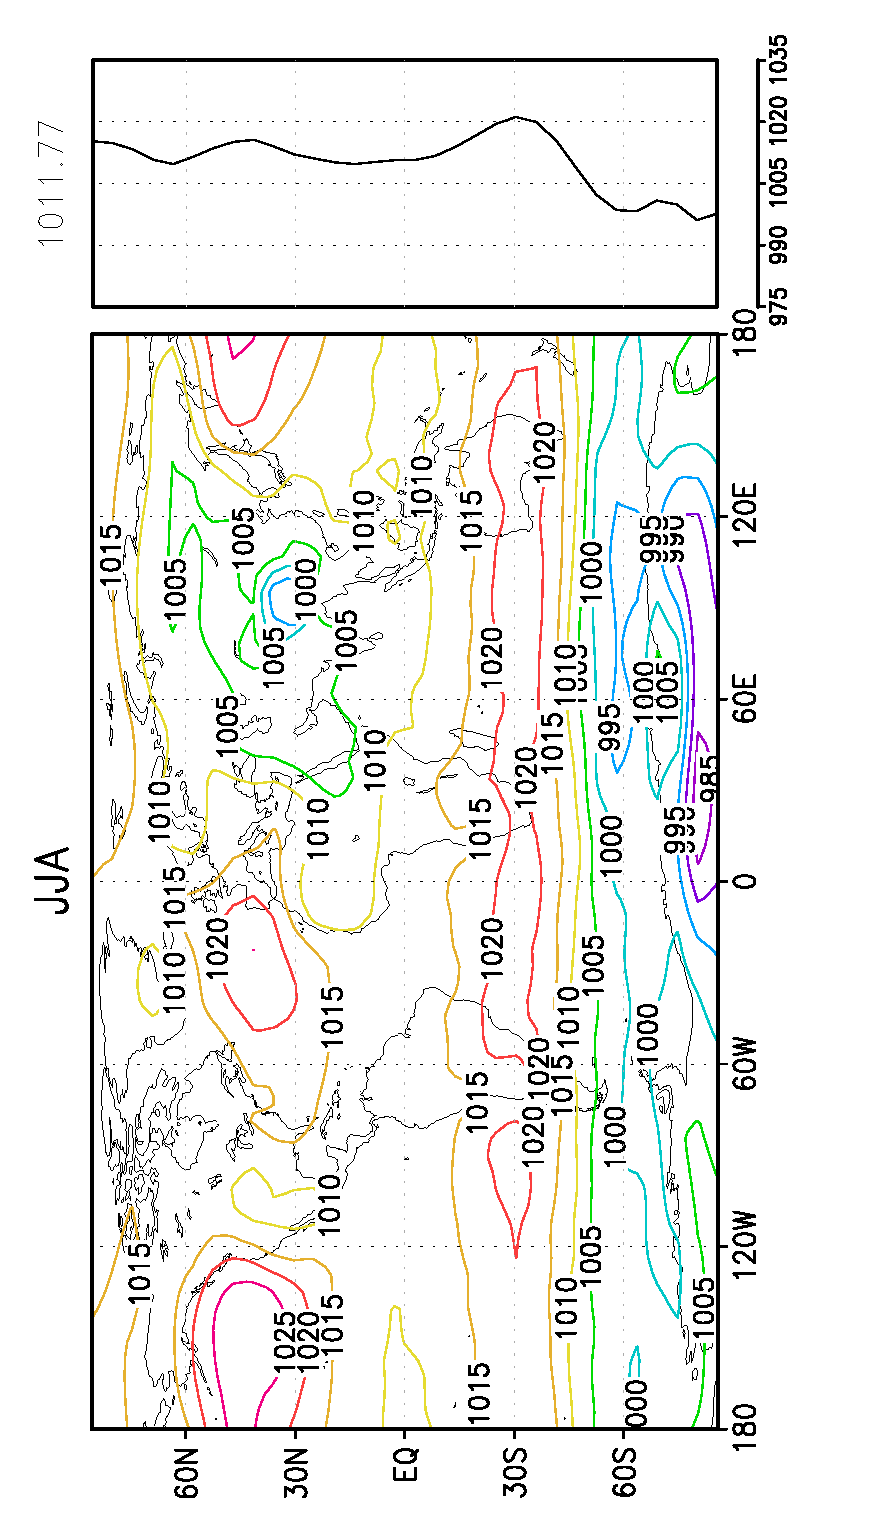
\includegraphics[height=8.5cm,width=6.5cm,angle=-90]
{eps/zonalfinalysmpres151JJA.eps}
}
\parbox{8.5cm}{\hspace{0.25cm}\begin{scriptsize}(e)\end{scriptsize} \vspace{-0.7cm} \\
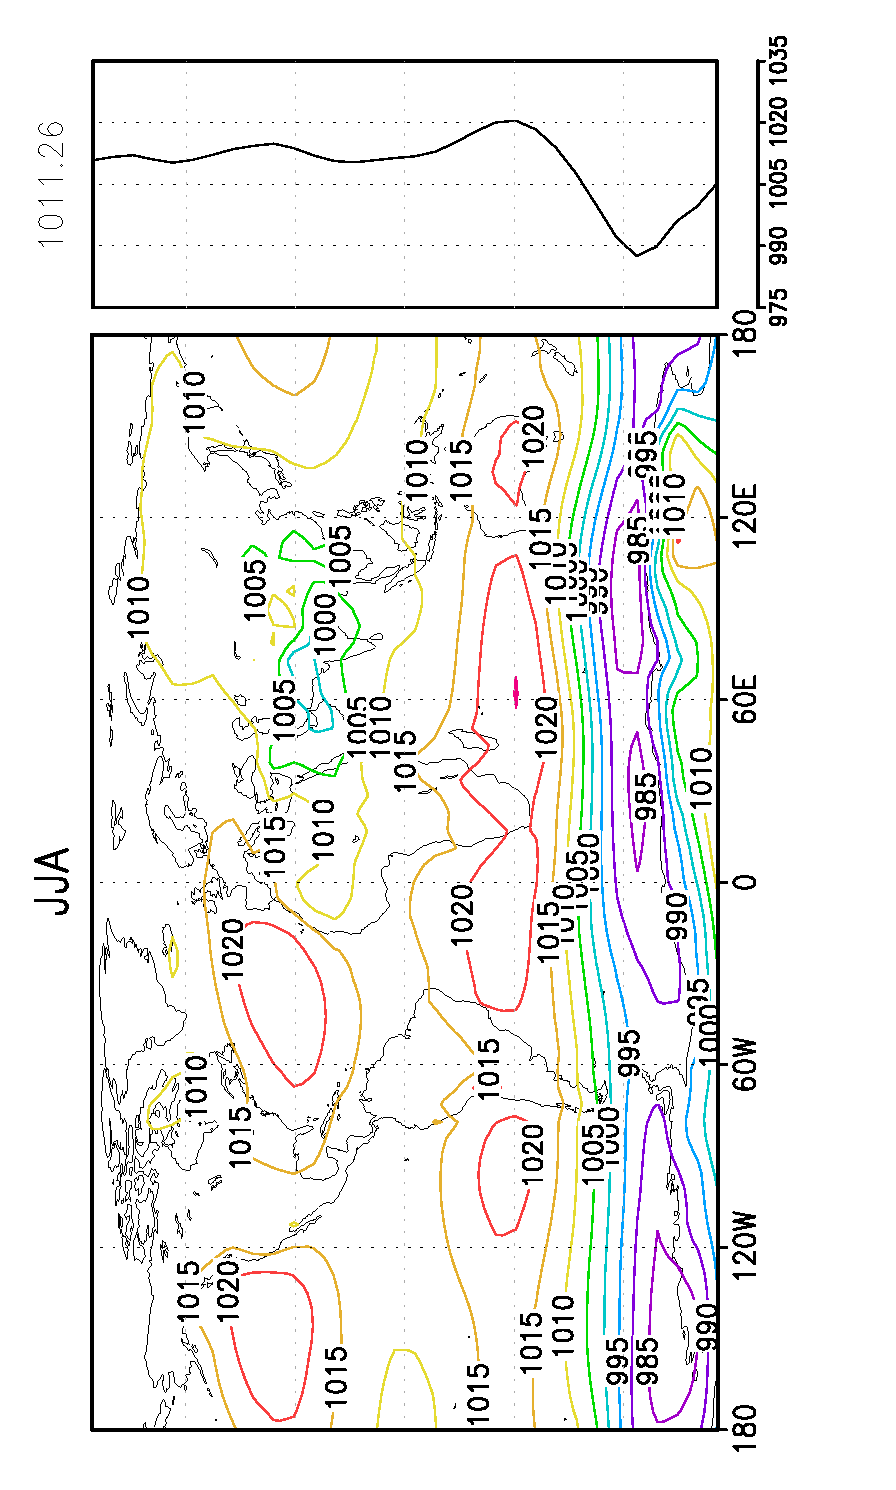
\includegraphics[height=8.5cm,width=6.5cm,angle=-90]
{eps/zonalt21finalysmmslpJJA.eps}
}
\parbox{8.5cm}{\hspace{0.50cm}\begin{scriptsize}(c)\end{scriptsize} \vspace{-0.7cm} \\
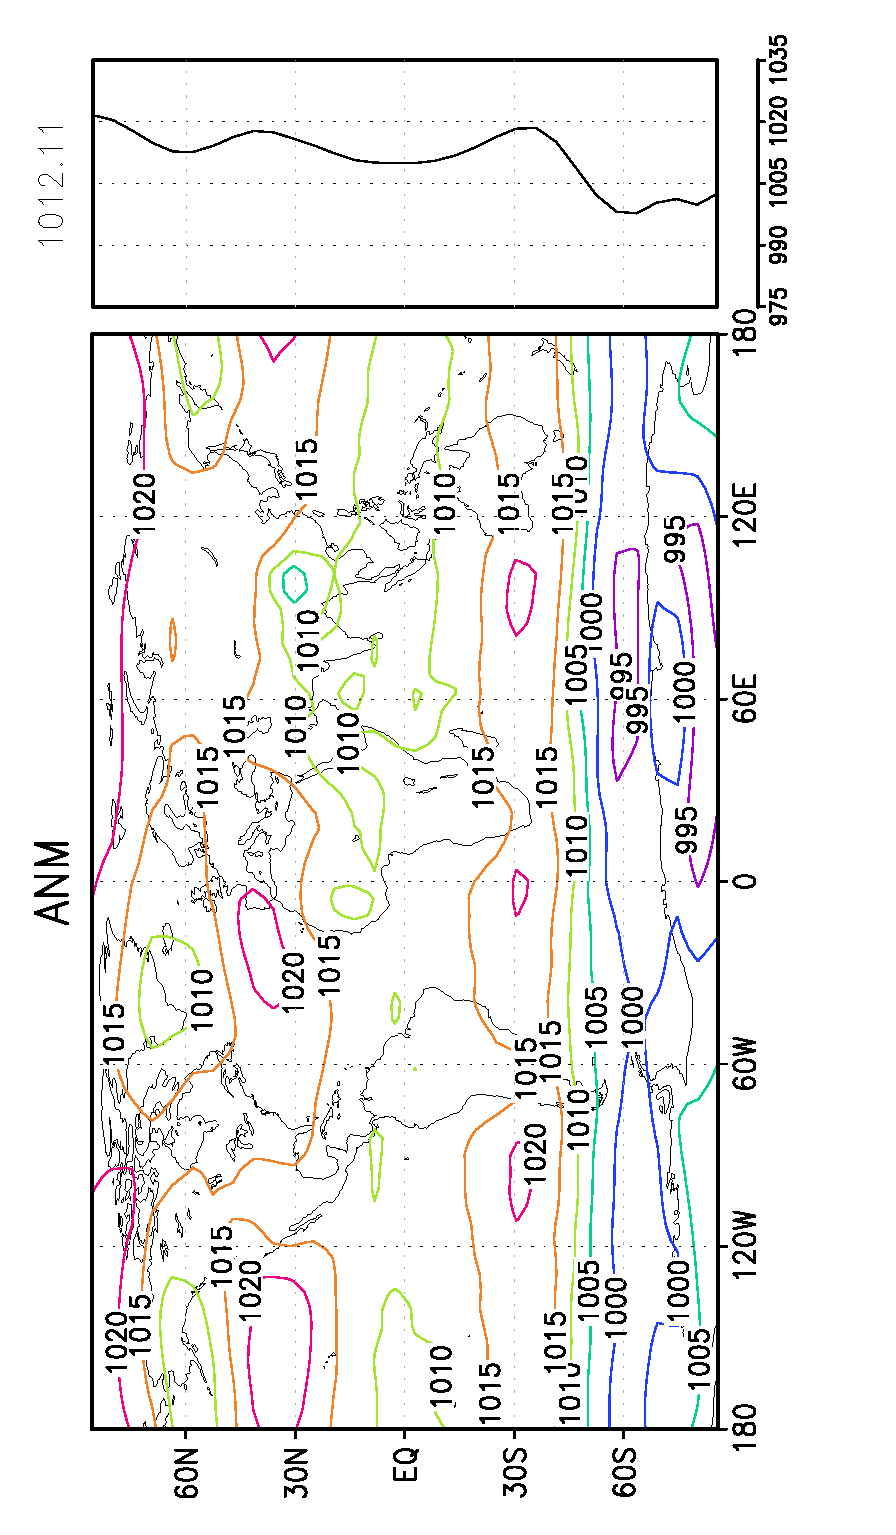
\includegraphics[height=8.5cm,width=6.5cm,angle=-90]
{eps/zonalfinaltmpres151.eps}
}
\parbox{8.5cm}{\hspace{0.25cm}\begin{scriptsize}(f)\end{scriptsize} \vspace{-0.7cm} \\
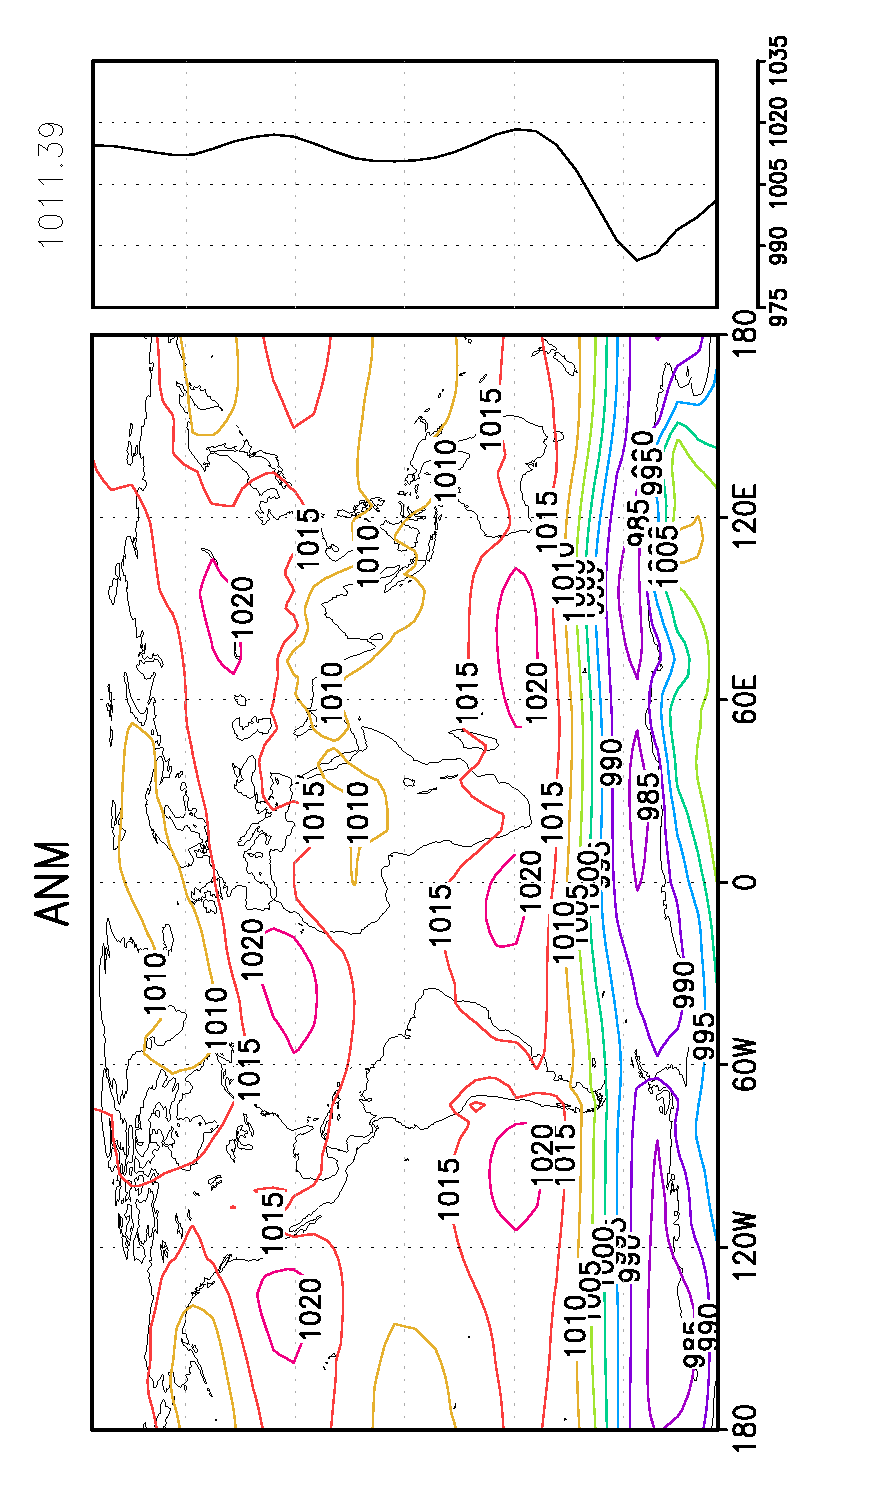
\includegraphics[height=8.5cm,width=6.5cm,angle=-90]
{eps/zonalt21finaltmmslp.eps}
}
\caption[Mean sea level pressure]{Mean sea level pressure [hPa]; right panels: zonal mean with global mean on top}
\label{img:mslp}
\end{figure}

\vspace{-0.4cm}
\section{Zonal winds (850 hPa)}
\vspace{-0.4cm}

In NH winter (Fig. \ref{img:u850} a, d), the 850 hPa wind shows a variable structure both in PlaSim and ERA. Meridional profiles (see Figures in appendix) are similar with two distinct maxima at about 40° N and 40° S; the NH maximum is stronger in PlaSim while the SH maximum is slightly weaker. During NH summer (Fig. \ref{img:u850} b), the easterly winds extend over the tropics except from the southern Indian Ocean to the tropical West Pacific. The westerlies of the Indian/Asian Monsoon are, compared to ERA (Fig. \ref{img:u850} e), less pronounced. The meridional profiles (see Figures in appendix) show the minimum near the equator and the maximum near 50° S.


\vspace{-0.4cm}
\section{Zonal winds (300 hPa)}
\vspace{-0.4cm}

Winds in NH winter (Fig. \ref{img:u300} a, d) show the two jets in each hemisphere. Jet maxima (35 $m/s$ and 50 $m/s$) are located near 30° N east of N-America and Asia; minima occur in the eastern Pacific and Atlantic. These features are captured by PlaSim and ERA. PlaSim shows stronger zonality and the jet is slightly shifted northward (see Figures in appendix) extending far into the eastern Pacific and Atlantic. The cross-Atlantic jet in PlaSim extends further eastward into central Europe while it continues to have a SW/NE orientation across the whole N-Atlantic in ERA. The equatorial easterlies are also stronger in PlaSim. The SH maximum is located near 45° S and more pronounced in PlaSim (35 $m/s$ to 30 $m/s$ in ERA). In NH summer (Fig. \ref{img:u300} b, e), wind maxima weaken; near 40° N they are about 15 $m/s$ (see Figures in appendix). In the SH, PlaSim overestimates the westerlies; the jet over Australia is stronger and located south of 30° S, while in ERA it is near 30° S.

\vspace{-0.4cm}
\section{Velocity potential (200 hPa)}
\vspace{-0.4cm}

The velocity potential of PlaSim and ERA shows large-scale maxima and minima over N-Africa, S-America and eastern Indonesia in NH winter (Fig. \ref{img:velopot200} a, d). During NH summer (Fig. \ref{img:velopot200} b, e), the winter-maximum over Africa shifts to the south-west into the Atlantic. The minimum over eastern Indonesia deepens and extends to the north-west. The annual mean (Fig. \ref{img:velopot200} c, f) shows the strong minimum in eastern Asia near the equator. Compared to ERA and \citet{Gates1999}, the winter-maximum over N-Africa and the minimum over Indonesia are less extended and their strength is underestimated in PlaSim, whereas the minimum over S-America is slightly too deep. During JJA, the maximum (minimum) is shifted too far to the west (north) and both are again underestimated in PlaSim. In the annual mean, the structures are more similar but the maxima and minima are still underestimated in PlaSim. As this parameter is connected to thermal circulations and convection in the tropics, the underestimation may indicate suppressed convection \citep{Gates1999}. 


\begin{figure}[H]
\hspace{3.8cm}PlaSim \vspace{0.2cm}\hspace{7.1cm} ERA \\
\parbox{8.5cm}{\hspace{0.50cm}\begin{scriptsize}(a)\end{scriptsize} \vspace{-0.7cm} \\
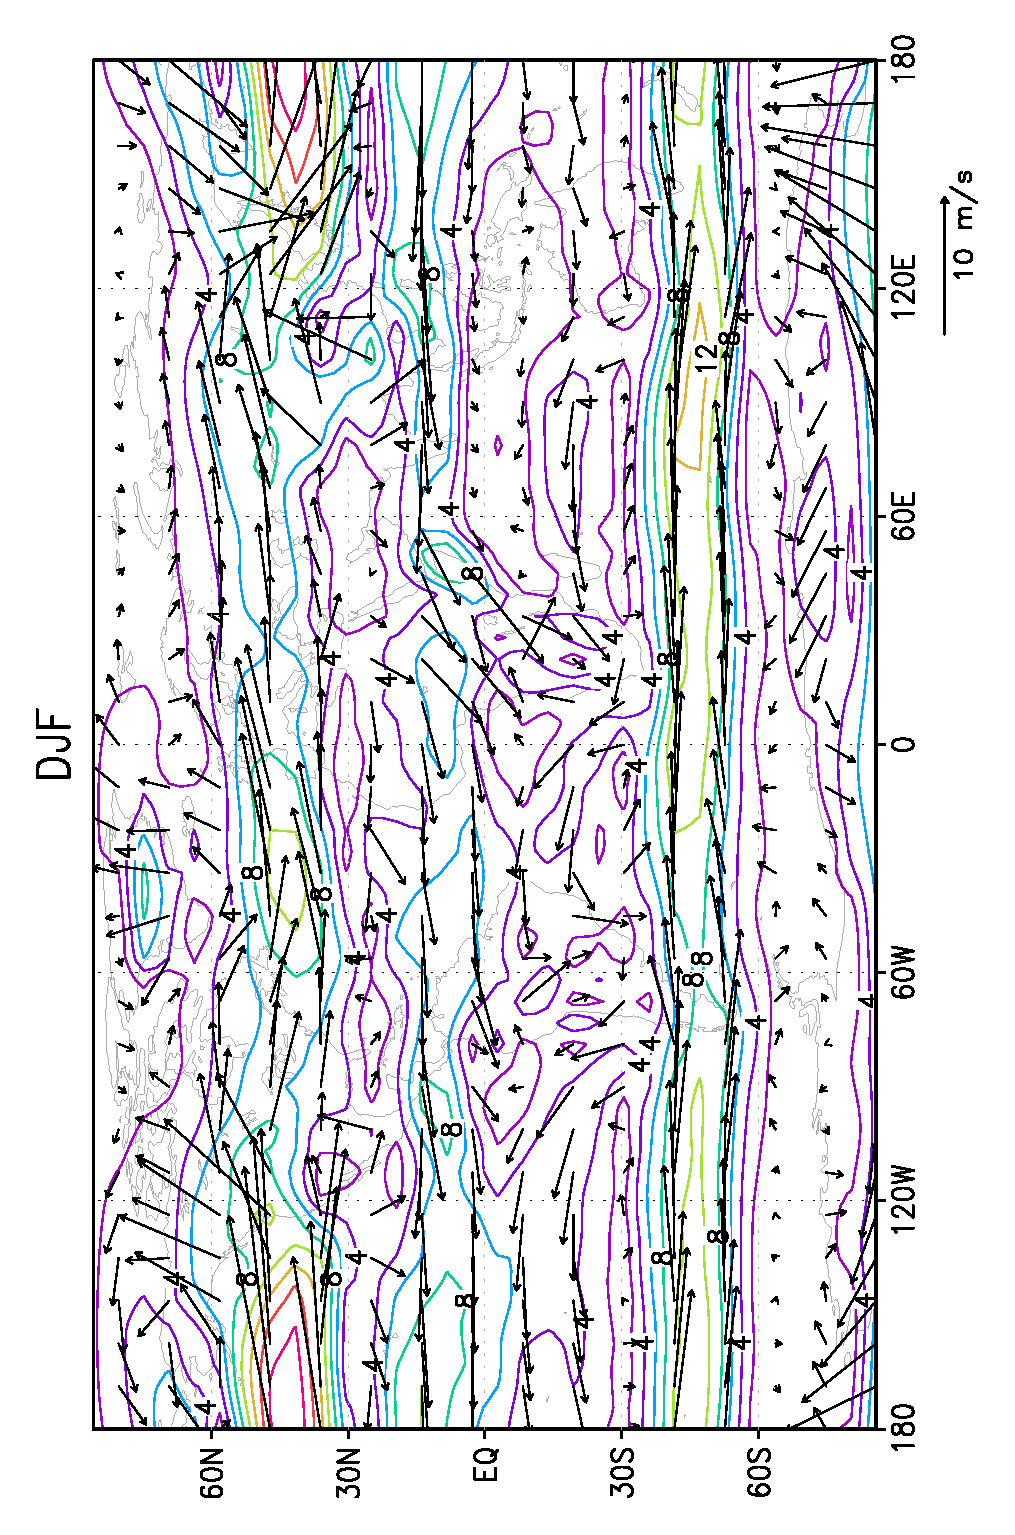
\includegraphics[height=8.5cm,width=6.5cm,angle=-90]
{eps/uv850DJF.eps}
}
\parbox{8.5cm}{\hspace{0.25cm}\begin{scriptsize}(d)\end{scriptsize} \vspace{-0.7cm} \\
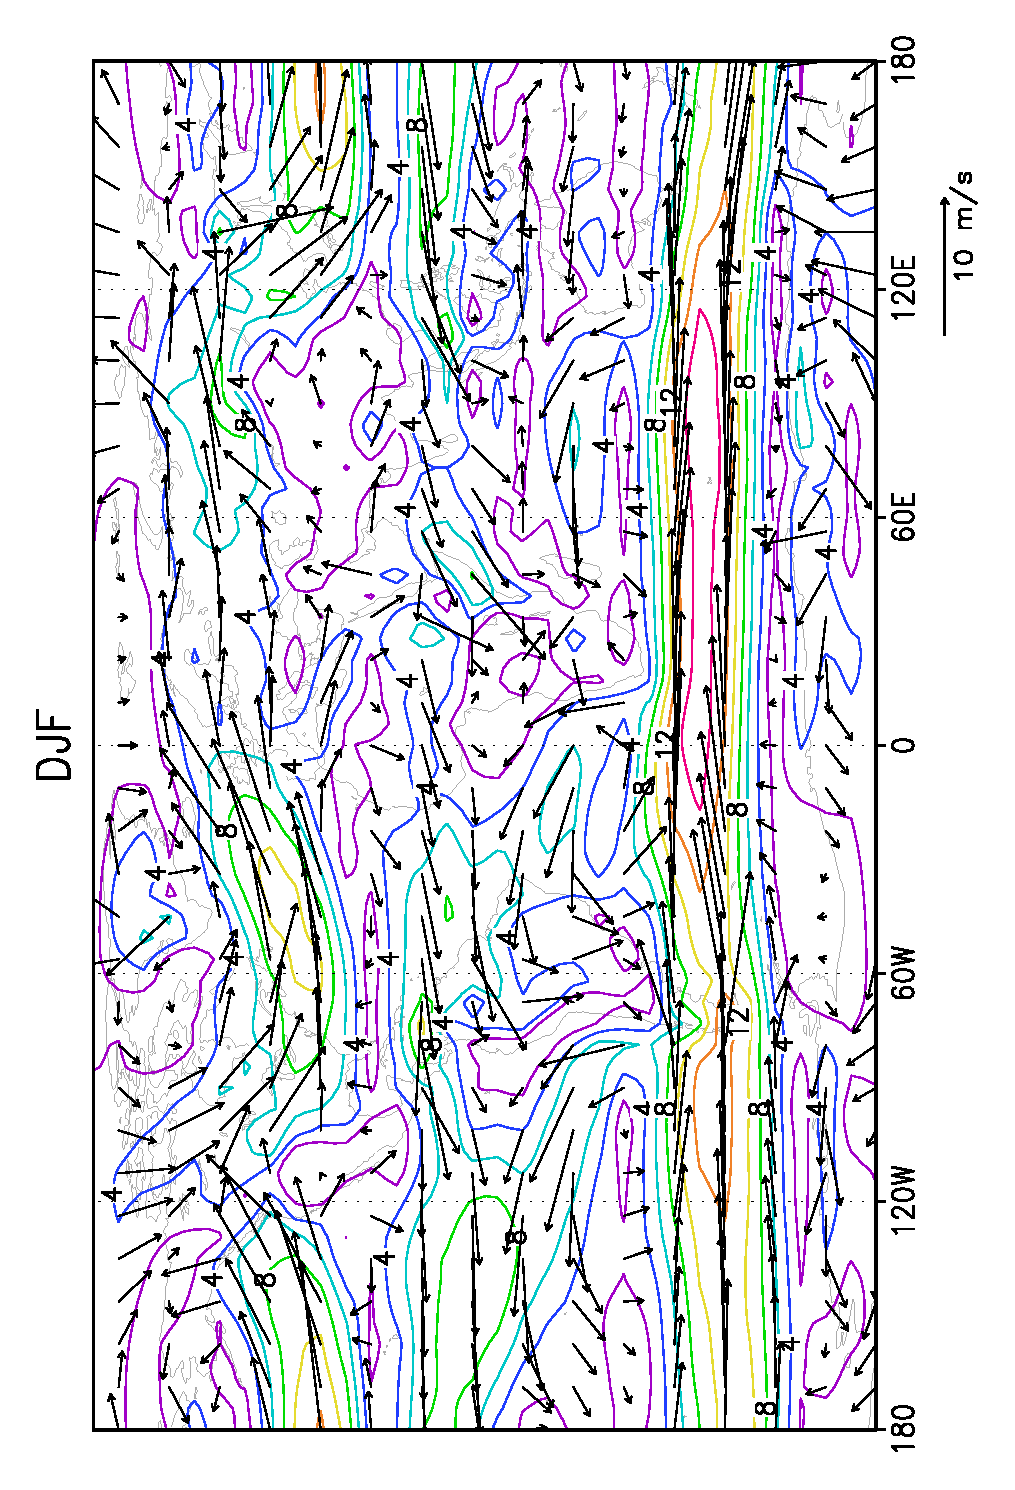
\includegraphics[height=8.5cm,width=6.5cm,angle=-90]
{eps/t21uv850DJF.eps}
}
\parbox{8.5cm}{\hspace{0.50cm}\begin{scriptsize}(b)\end{scriptsize} \vspace{-0.7cm} \\
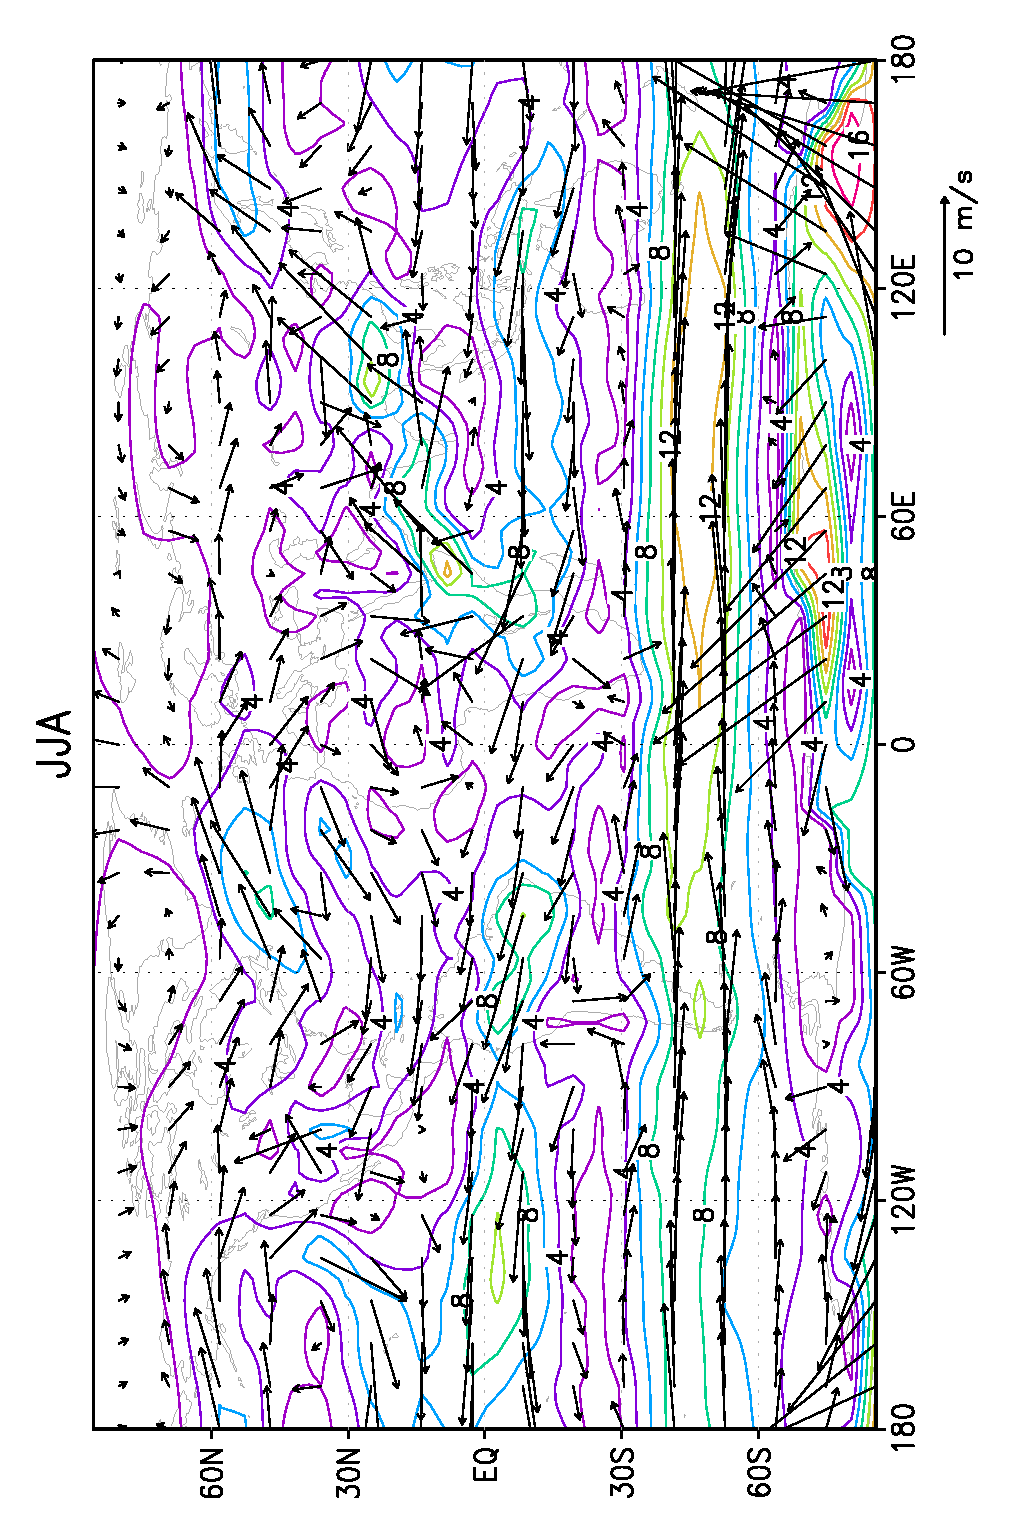
\includegraphics[height=8.5cm,width=6.5cm,angle=-90]
{eps/uv850JJA.eps}
}
\parbox{8.5cm}{\hspace{0.25cm}\begin{scriptsize}(e)\end{scriptsize} \vspace{-0.7cm} \\
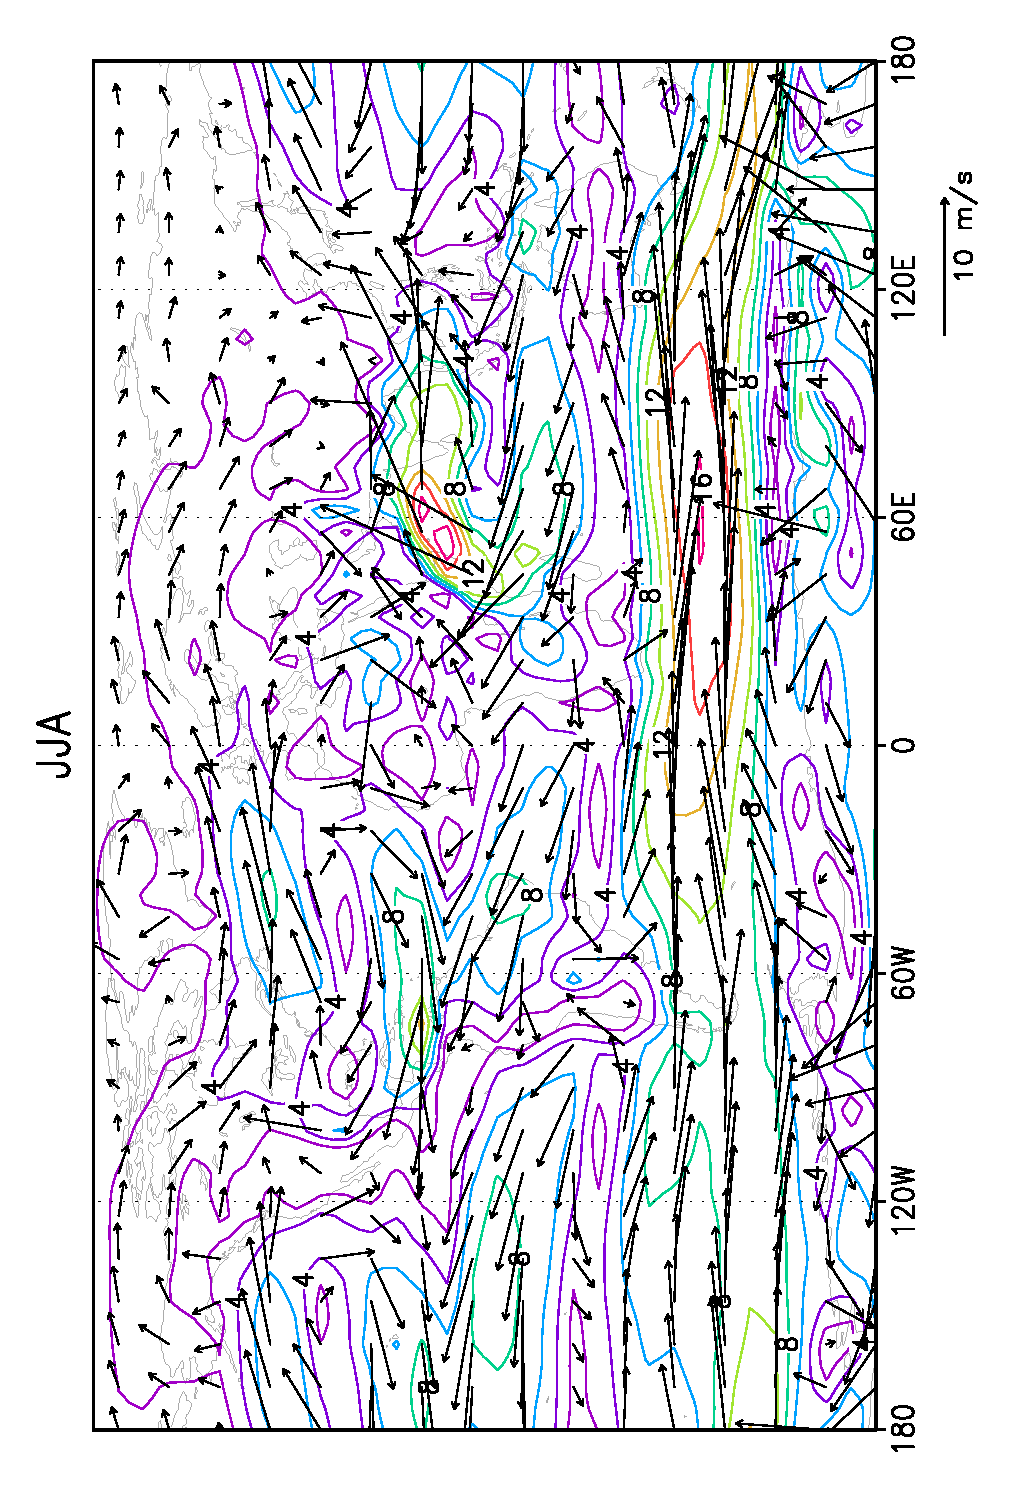
\includegraphics[height=8.5cm,width=6.5cm,angle=-90]
{eps/t21uv850JJA.eps}
}
\parbox{8.5cm}{\hspace{0.50cm}\begin{scriptsize}(c)\end{scriptsize} \vspace{-0.7cm} \\
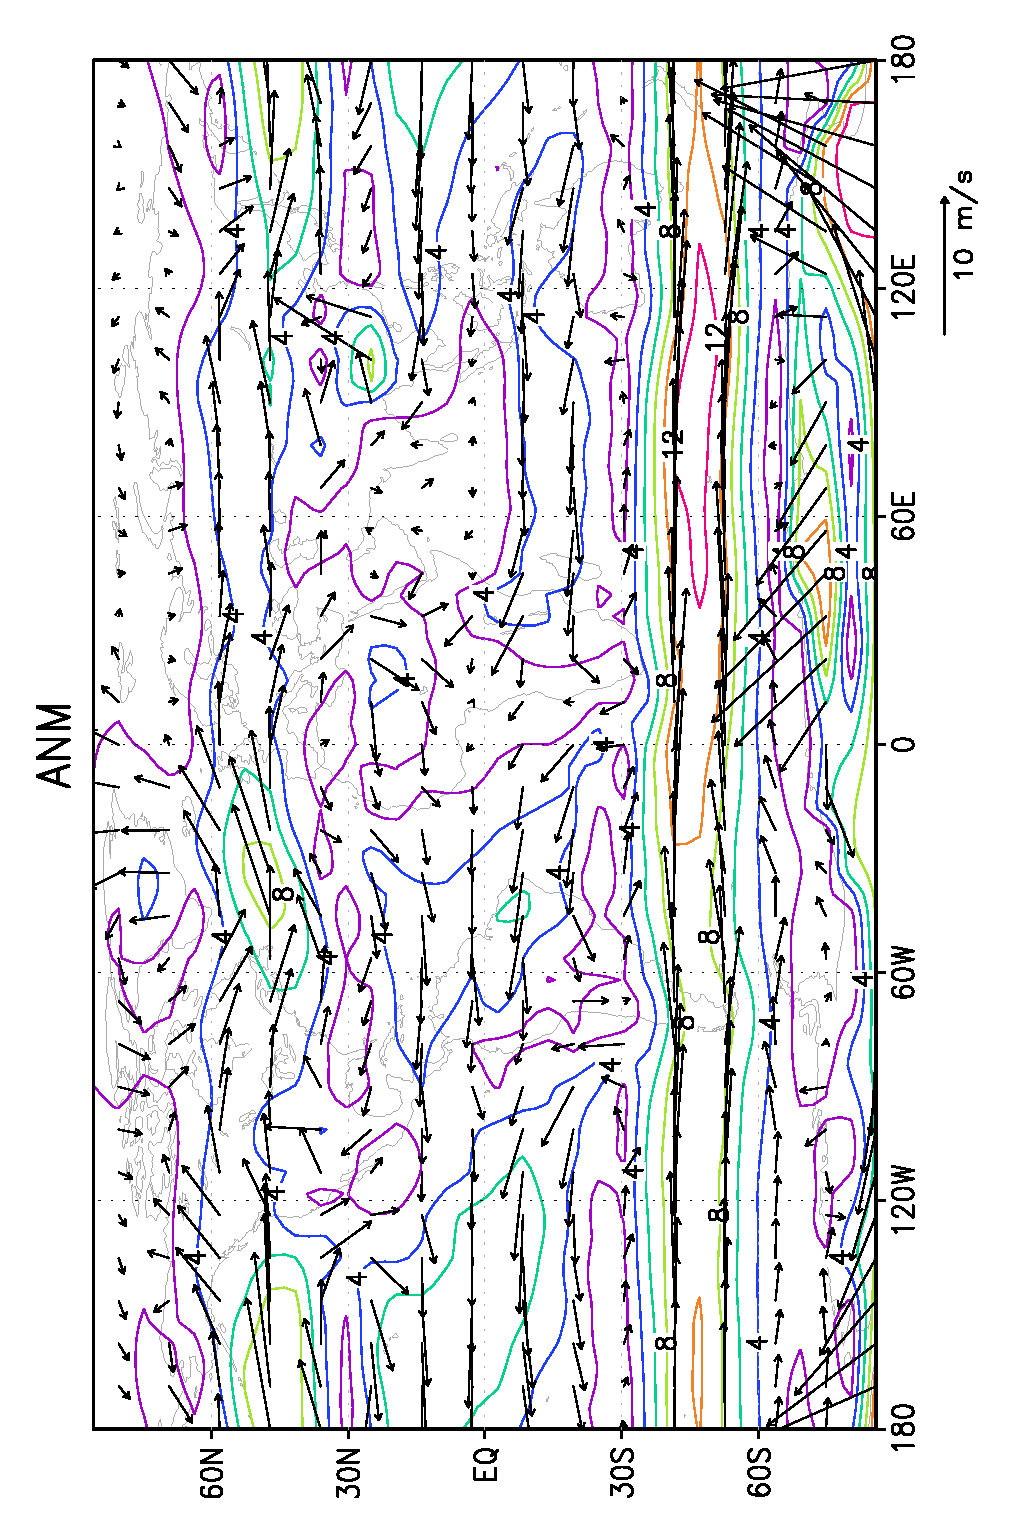
\includegraphics[height=8.5cm,width=6.5cm,angle=-90]
{eps/tmuv850.eps}
}
\parbox{8.5cm}{\hspace{0.25cm}\begin{scriptsize}(f)\end{scriptsize} \vspace{-0.7cm} \\
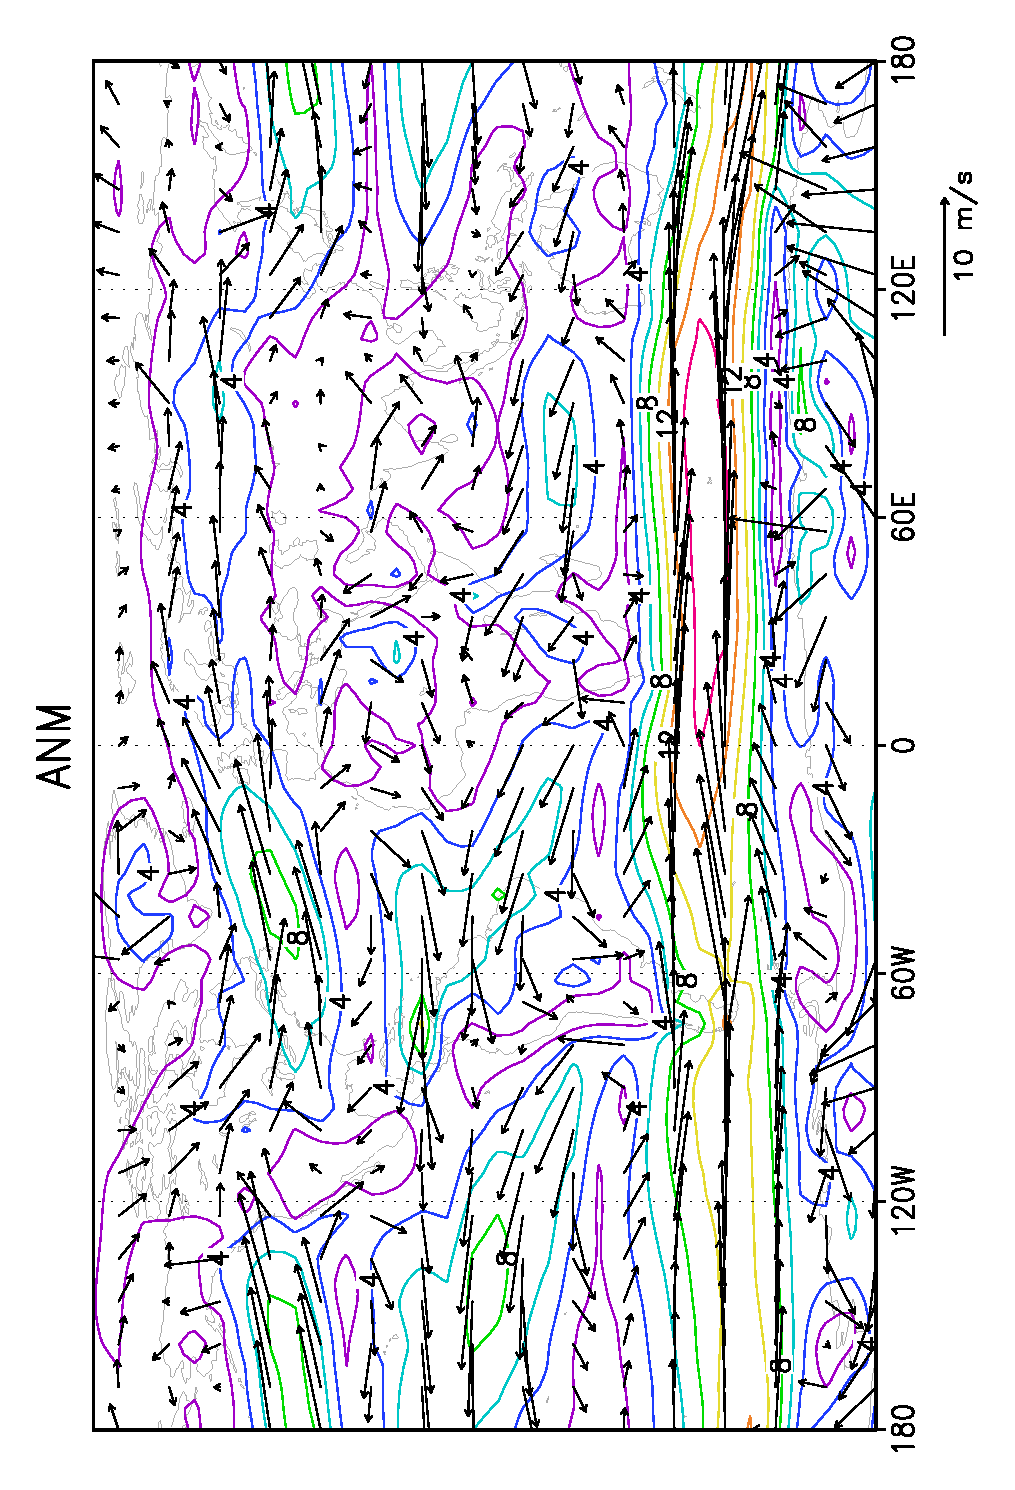
\includegraphics[height=8.5cm,width=6.5cm,angle=-90]
{eps/t21tmuv850.eps}
}
\caption[Wind at 850 hPa]{Wind at 850 hPa [m/s]; wind vectors (arrows) and windspeed (isolines)}
\label{img:u850}
\end{figure}


\begin{figure}[H]
\hspace{3.8cm}PlaSim \vspace{0.2cm}\hspace{7.1cm} ERA \\
\parbox{8.5cm}{\hspace{0.50cm}\begin{scriptsize}(a)\end{scriptsize} \vspace{-0.7cm} \\
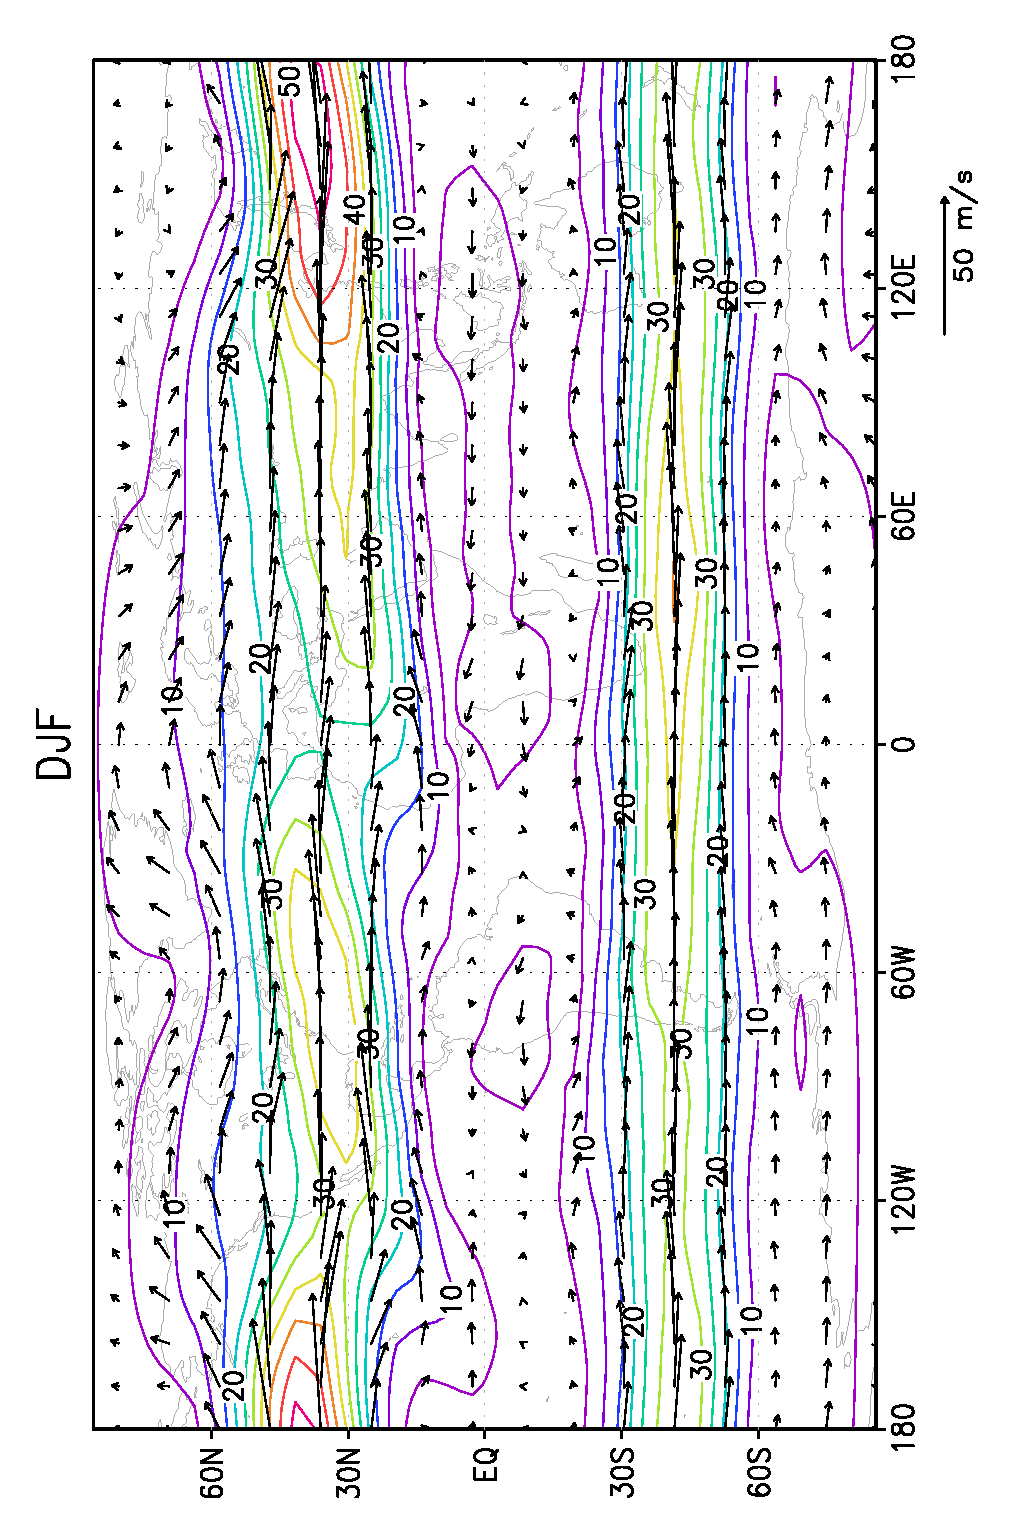
\includegraphics[height=8.5cm,width=6.5cm,angle=-90]
{eps/uv300DJF.eps}
}
\parbox{8.5cm}{\hspace{0.25cm}\begin{scriptsize}(d)\end{scriptsize} \vspace{-0.7cm} \\
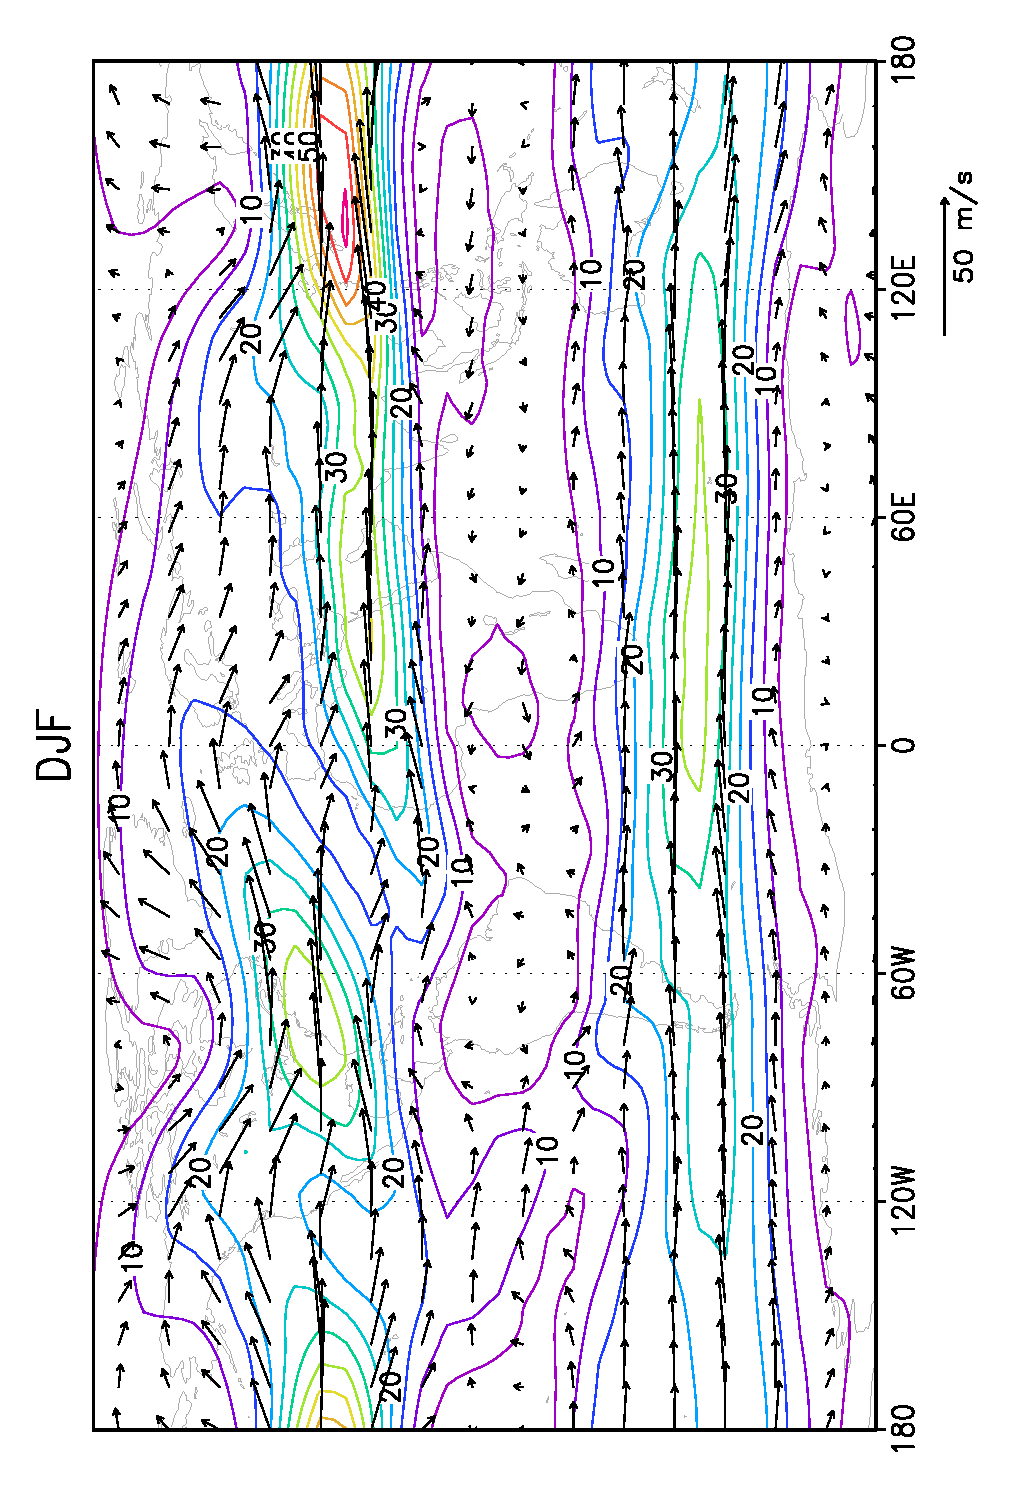
\includegraphics[height=8.5cm,width=6.5cm,angle=-90]
{eps/t21uv300DJF.eps}
}
\parbox{8.5cm}{\hspace{0.50cm}\begin{scriptsize}(b)\end{scriptsize} \vspace{-0.7cm} \\
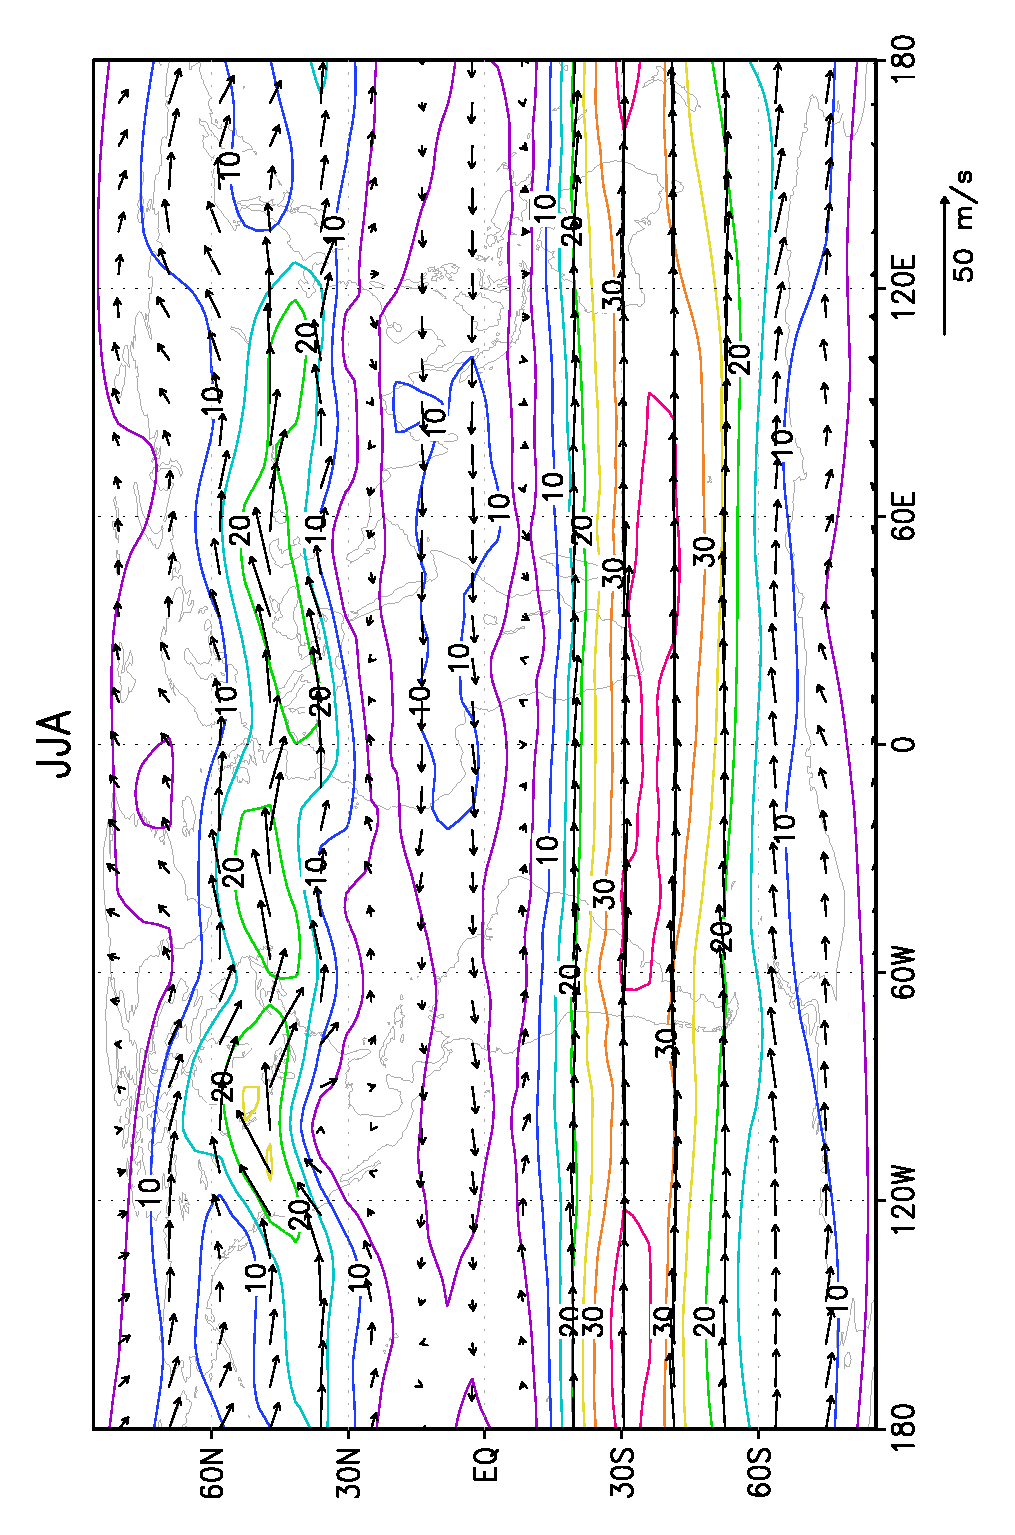
\includegraphics[height=8.5cm,width=6.5cm,angle=-90]
{eps/uv300JJA.eps}
}
\parbox{8.5cm}{\hspace{0.25cm}\begin{scriptsize}(e)\end{scriptsize} \vspace{-0.7cm} \\
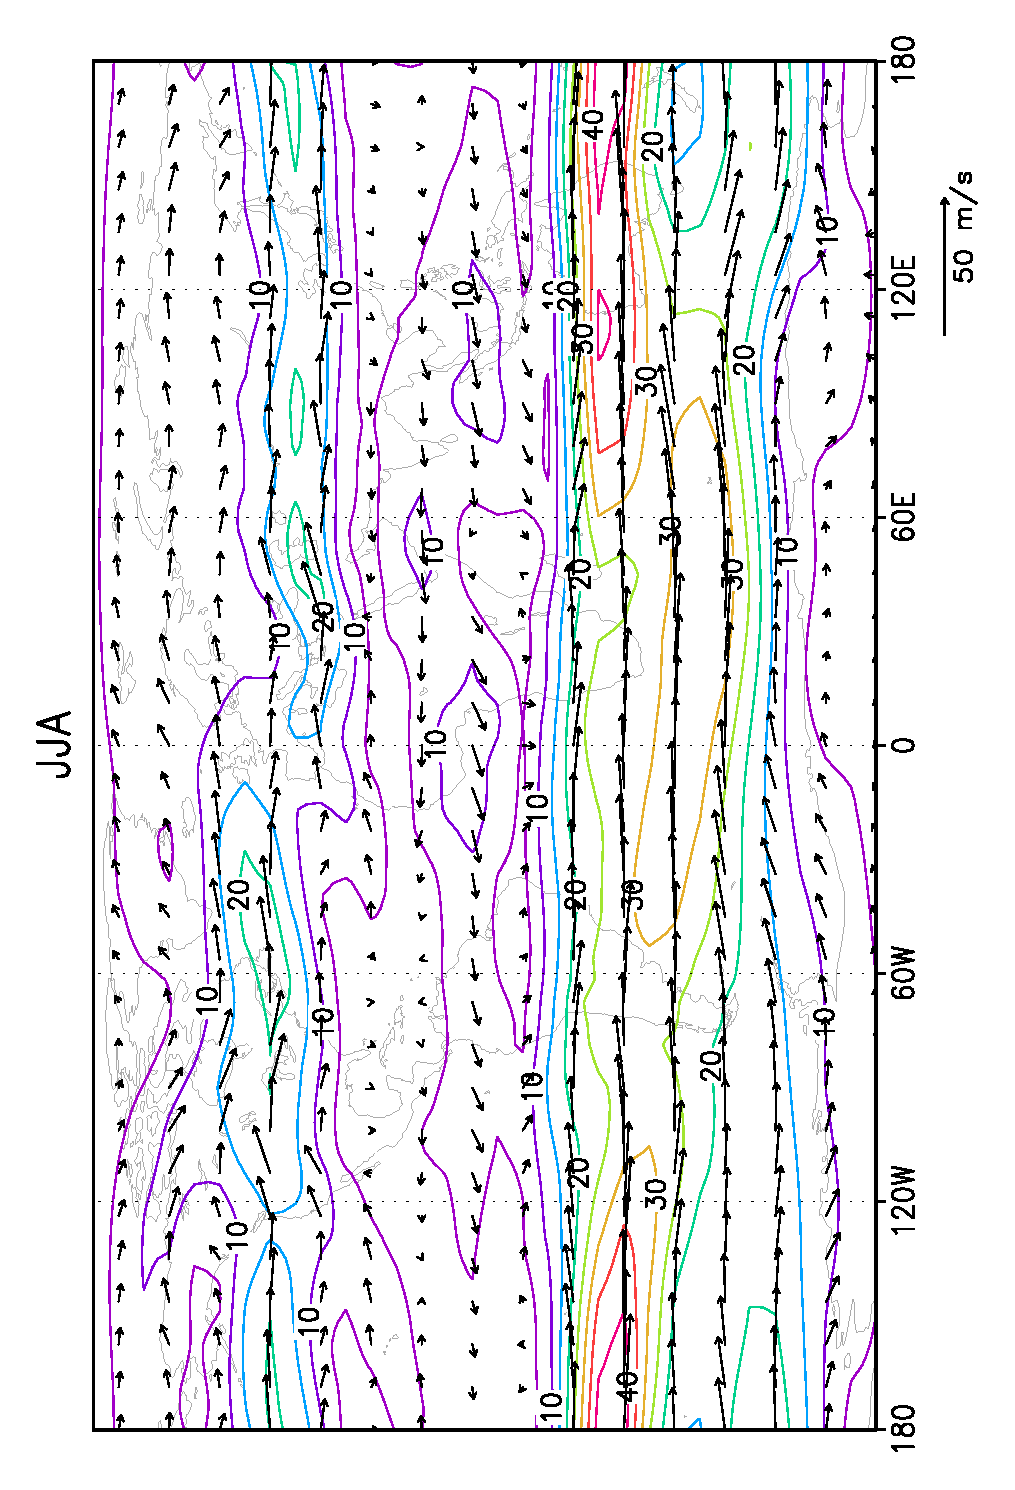
\includegraphics[height=8.5cm,width=6.5cm,angle=-90]
{eps/t21uv300JJA.eps}
}
\parbox{8.5cm}{\hspace{0.50cm}\begin{scriptsize}(c)\end{scriptsize} \vspace{-0.7cm} \\
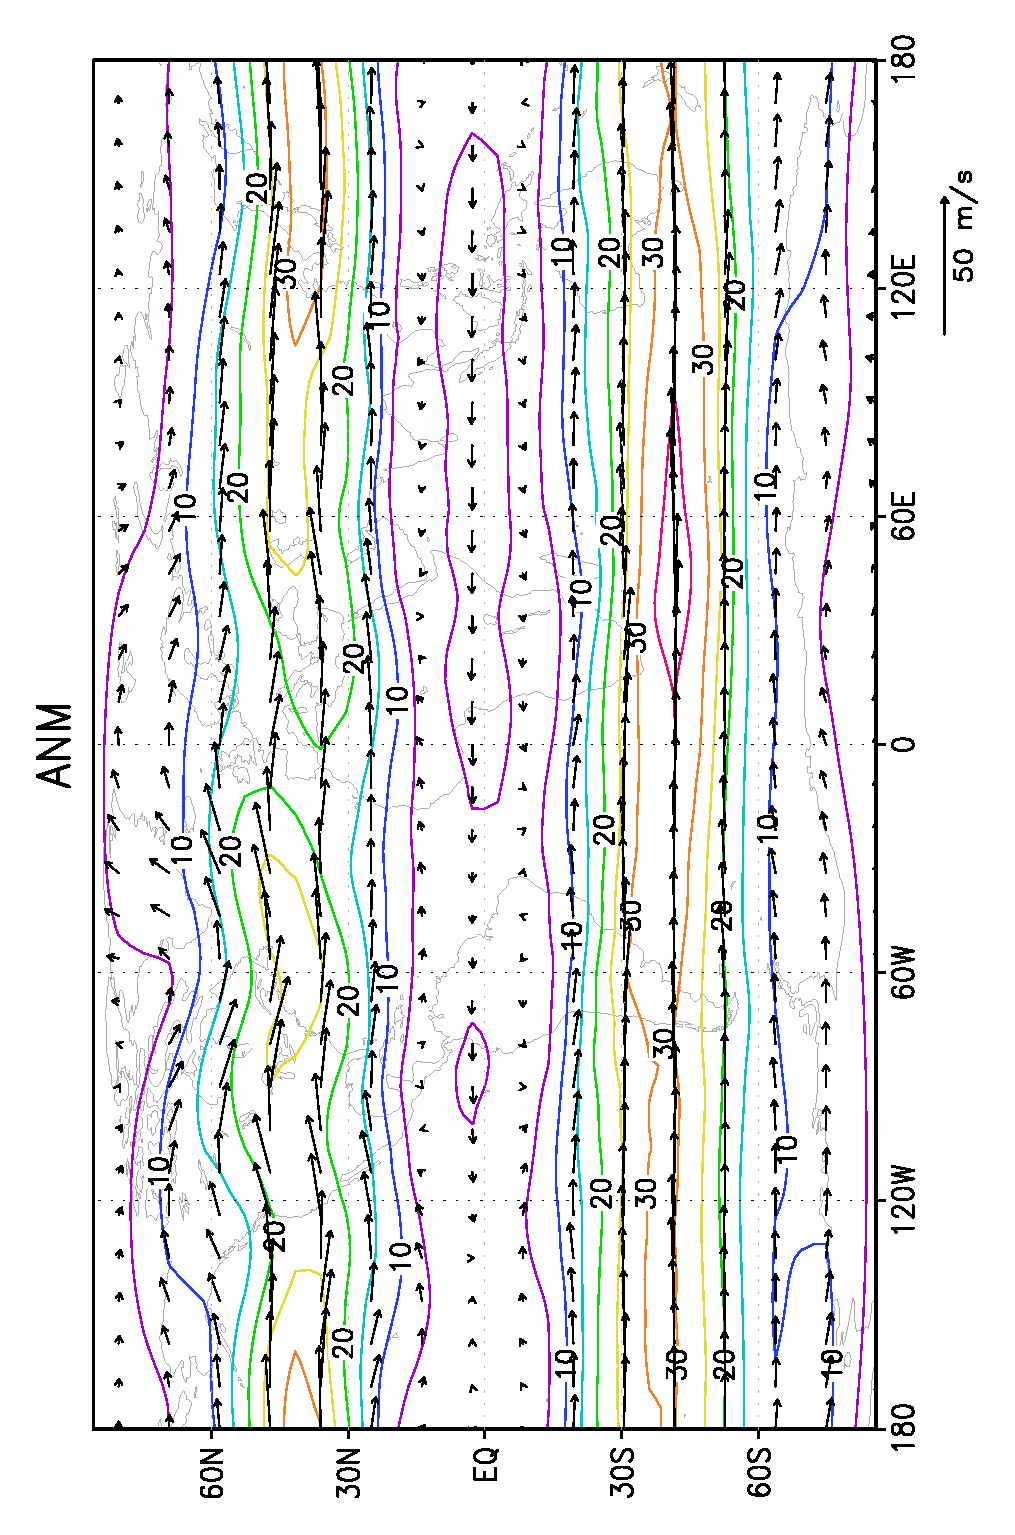
\includegraphics[height=8.5cm,width=6.5cm,angle=-90]
{eps/tmuv300.eps}
}
\parbox{8.5cm}{\hspace{0.25cm}\begin{scriptsize}(f)\end{scriptsize} \vspace{-0.7cm} \\
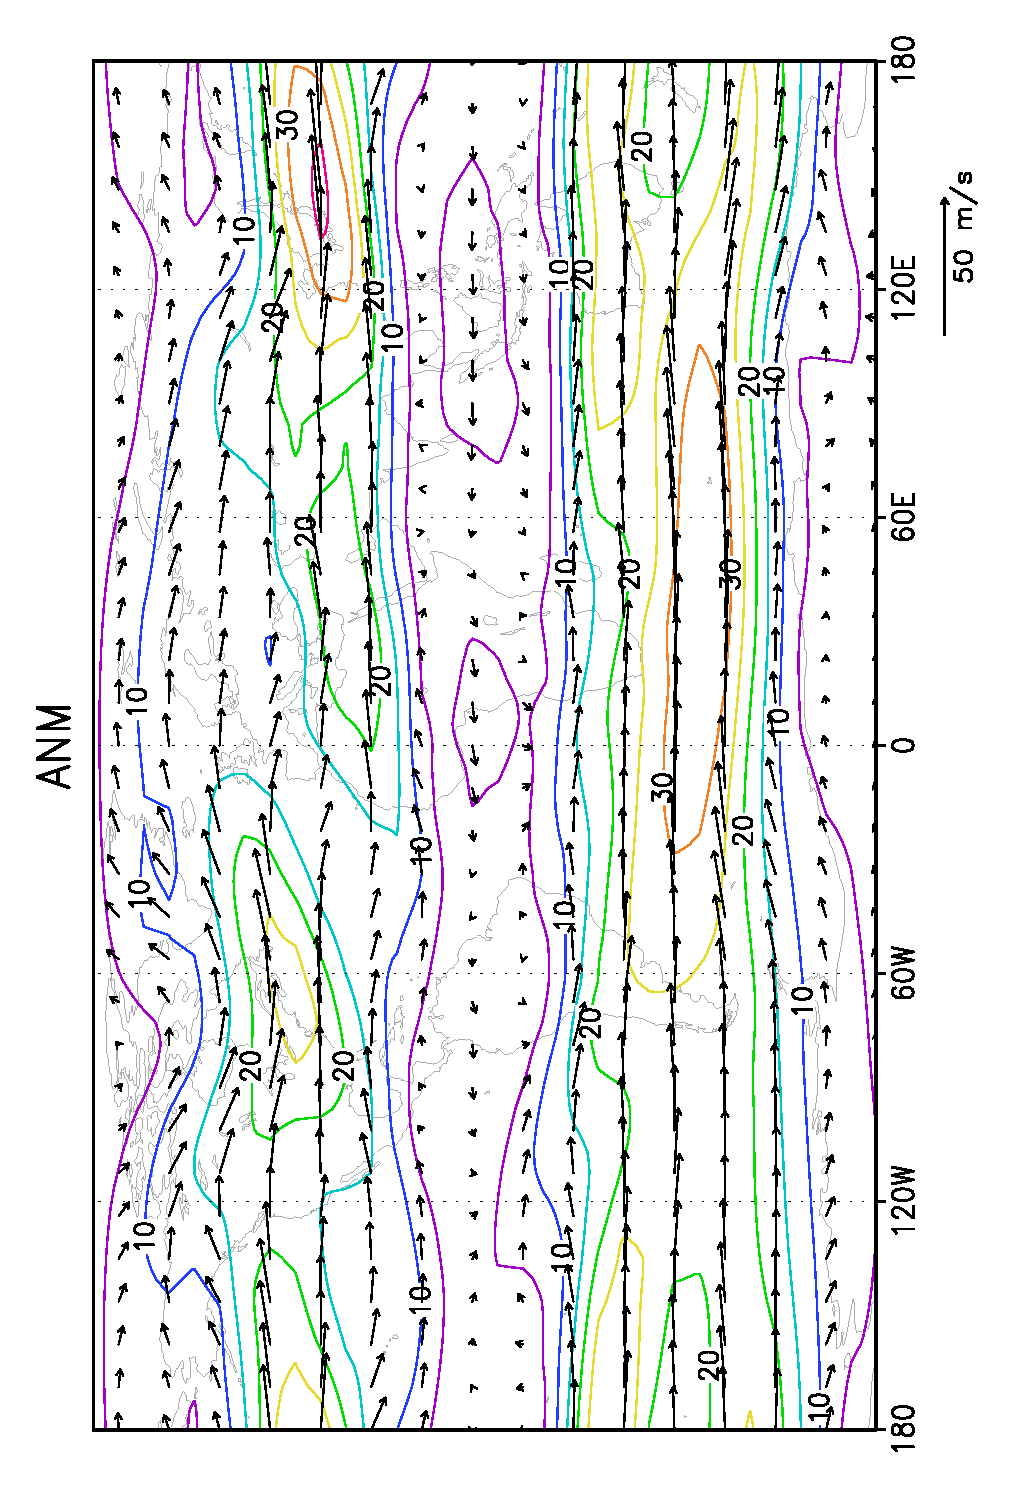
\includegraphics[height=8.5cm,width=6.5cm,angle=-90]
{eps/t21tmuv300.eps}
}
\caption[Wind at 300 hPa]{Wind at 300 hPa [m/s]; wind vectors (arrows) and windspeed (isolines)}
\label{img:u300}
\end{figure}


\begin{figure}[H]
\hspace{3.8cm}PlaSim \vspace{0.2cm}\hspace{7.2cm} ERA \\
\parbox{8.5cm}{\hspace{0.50cm}\begin{scriptsize}(a)\end{scriptsize} \vspace{-0.7cm} \\
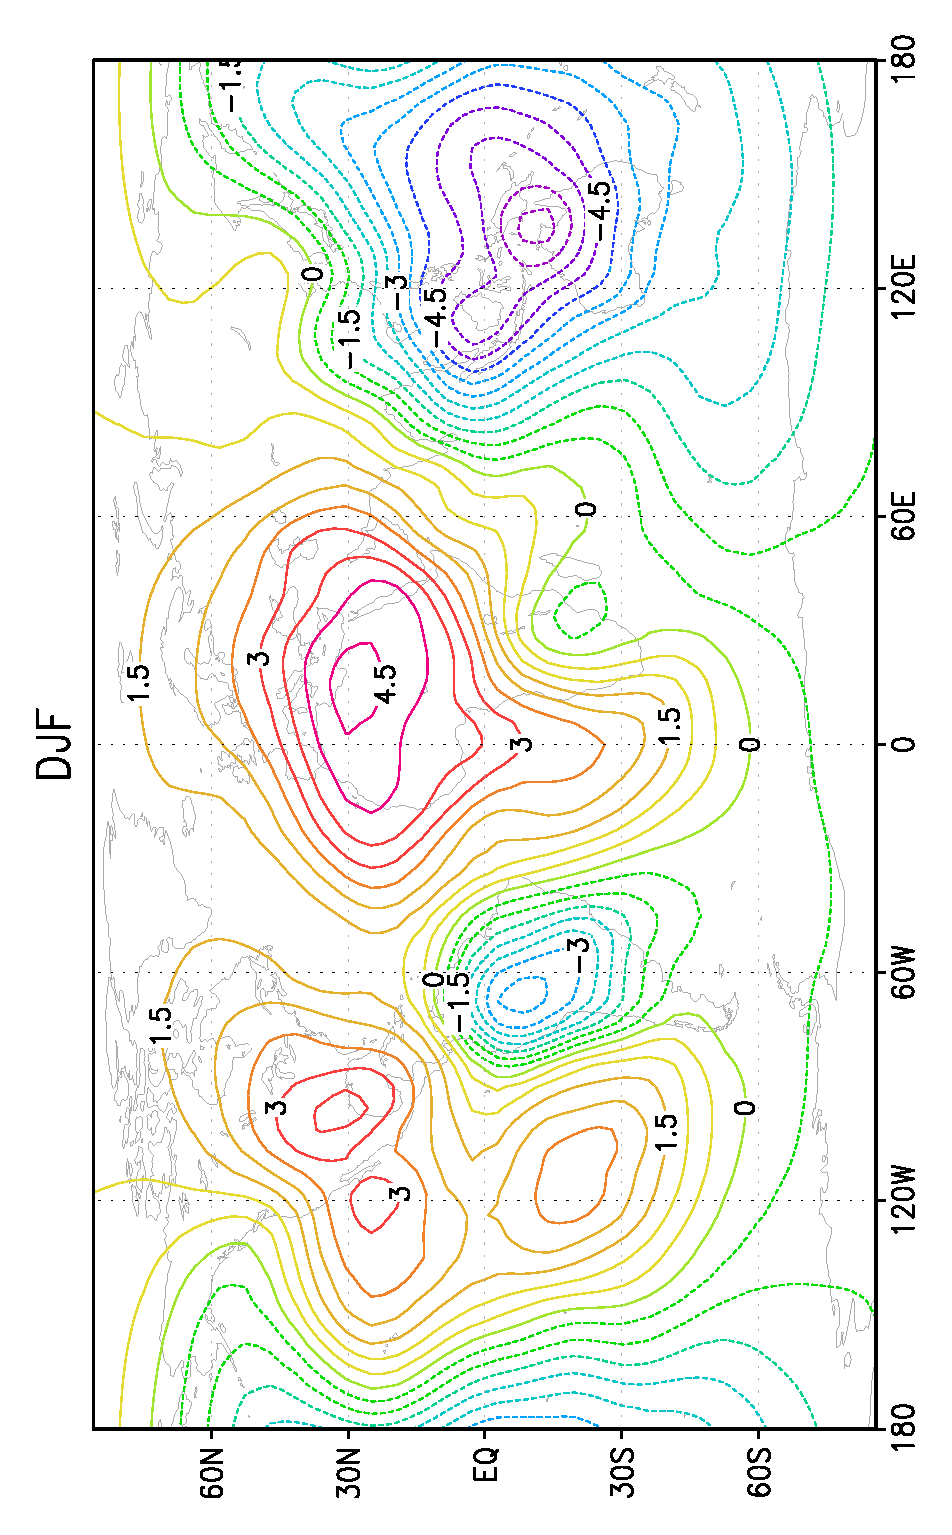
\includegraphics[height=8.5cm,width=6.1cm,angle=-90]
{eps/finalysmvelopot149_200DJF.eps}
}
\parbox{8.5cm}{\hspace{0.25cm}\begin{scriptsize}(d)\end{scriptsize} \vspace{-0.7cm} \\
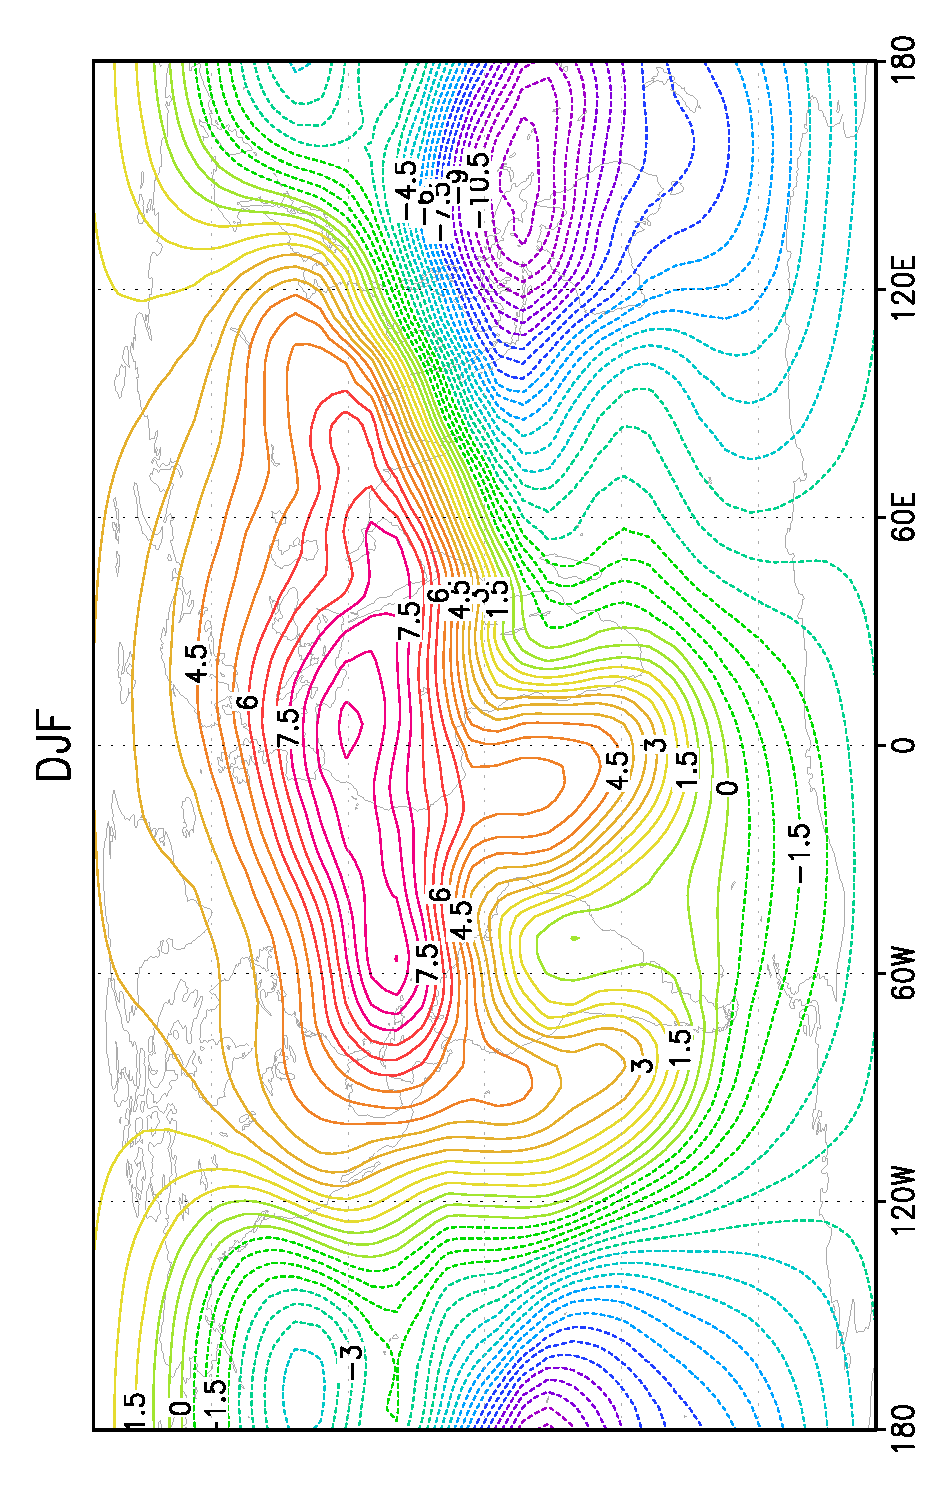
\includegraphics[height=8.5cm,width=6.1cm,angle=-90]
{eps/finalysmt21_ERA40VELPOT200DJF.eps}
}
\parbox{8.5cm}{\hspace{0.50cm}\begin{scriptsize}(b)\end{scriptsize} \vspace{-0.8cm} \\
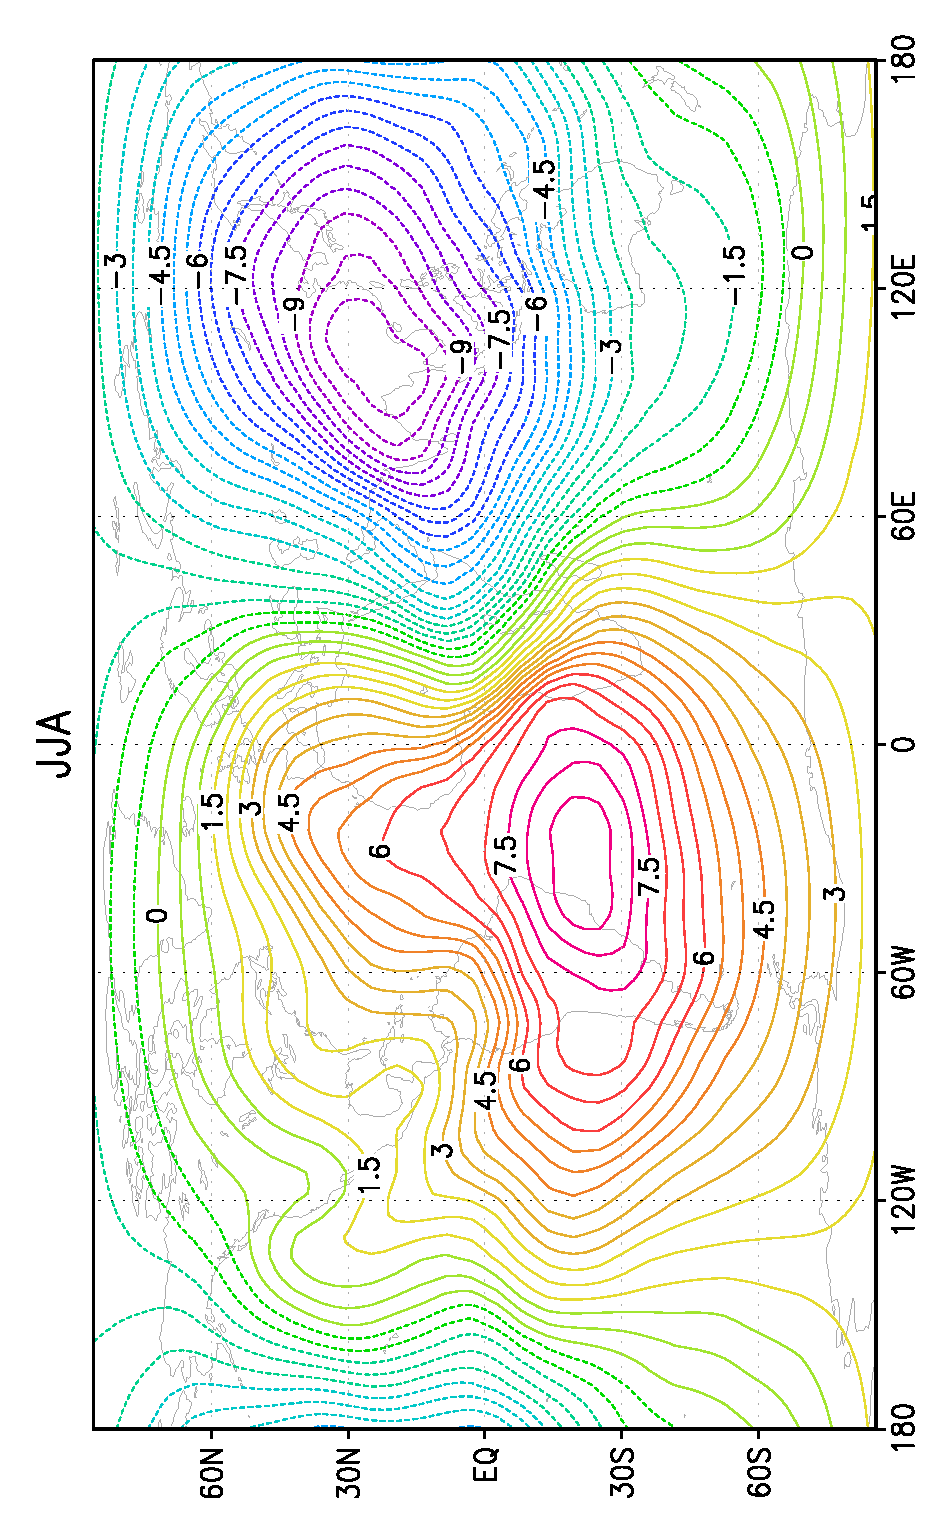
\includegraphics[height=8.5cm,width=6.1cm,angle=-90]
{eps/finalysmvelopot149_200JJA.eps}
}
\parbox{8.5cm}{\hspace{0.25cm}\begin{scriptsize}(e)\end{scriptsize} \vspace{-0.8cm} \\
\includegraphics[height=8.5cm,width=6.1cm,angle=-90]
{eps/finalysmt21_ERA40VELPOT200JJA.eps}
}
\parbox{8.5cm}{\hspace{0.50cm}\begin{scriptsize}(c)\end{scriptsize} \vspace{-0.8cm} \\
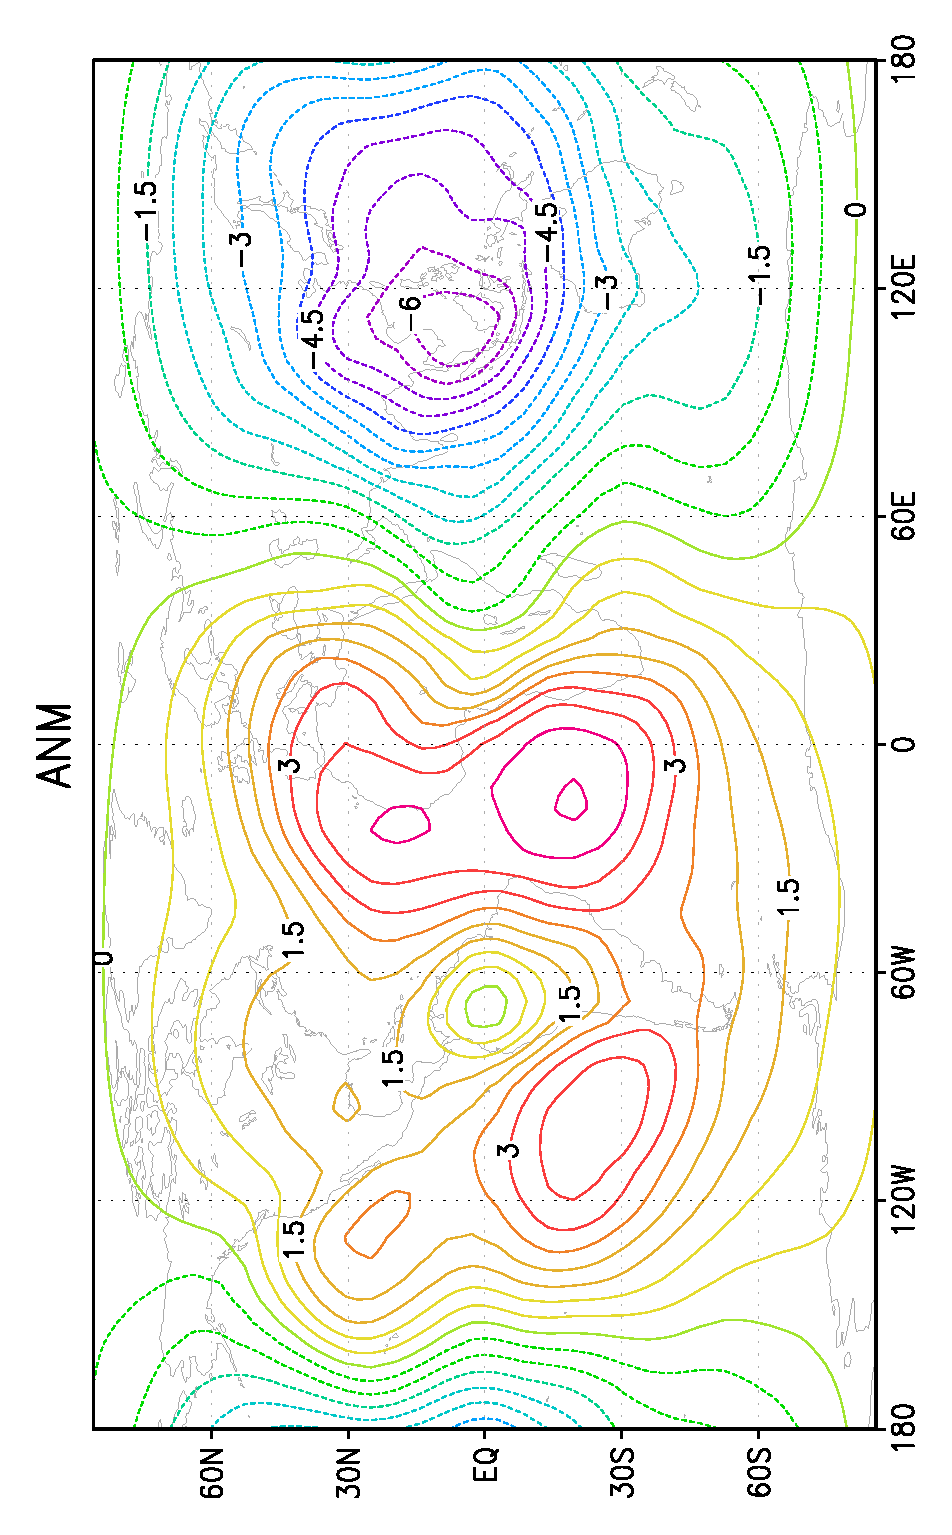
\includegraphics[height=8.5cm,width=6.1cm,angle=-90]
{eps/finaltmvelopot149_200.eps}
}
\parbox{8.5cm}{\hspace{0.25cm}\begin{scriptsize}(f)\end{scriptsize} \vspace{-0.8cm} \\
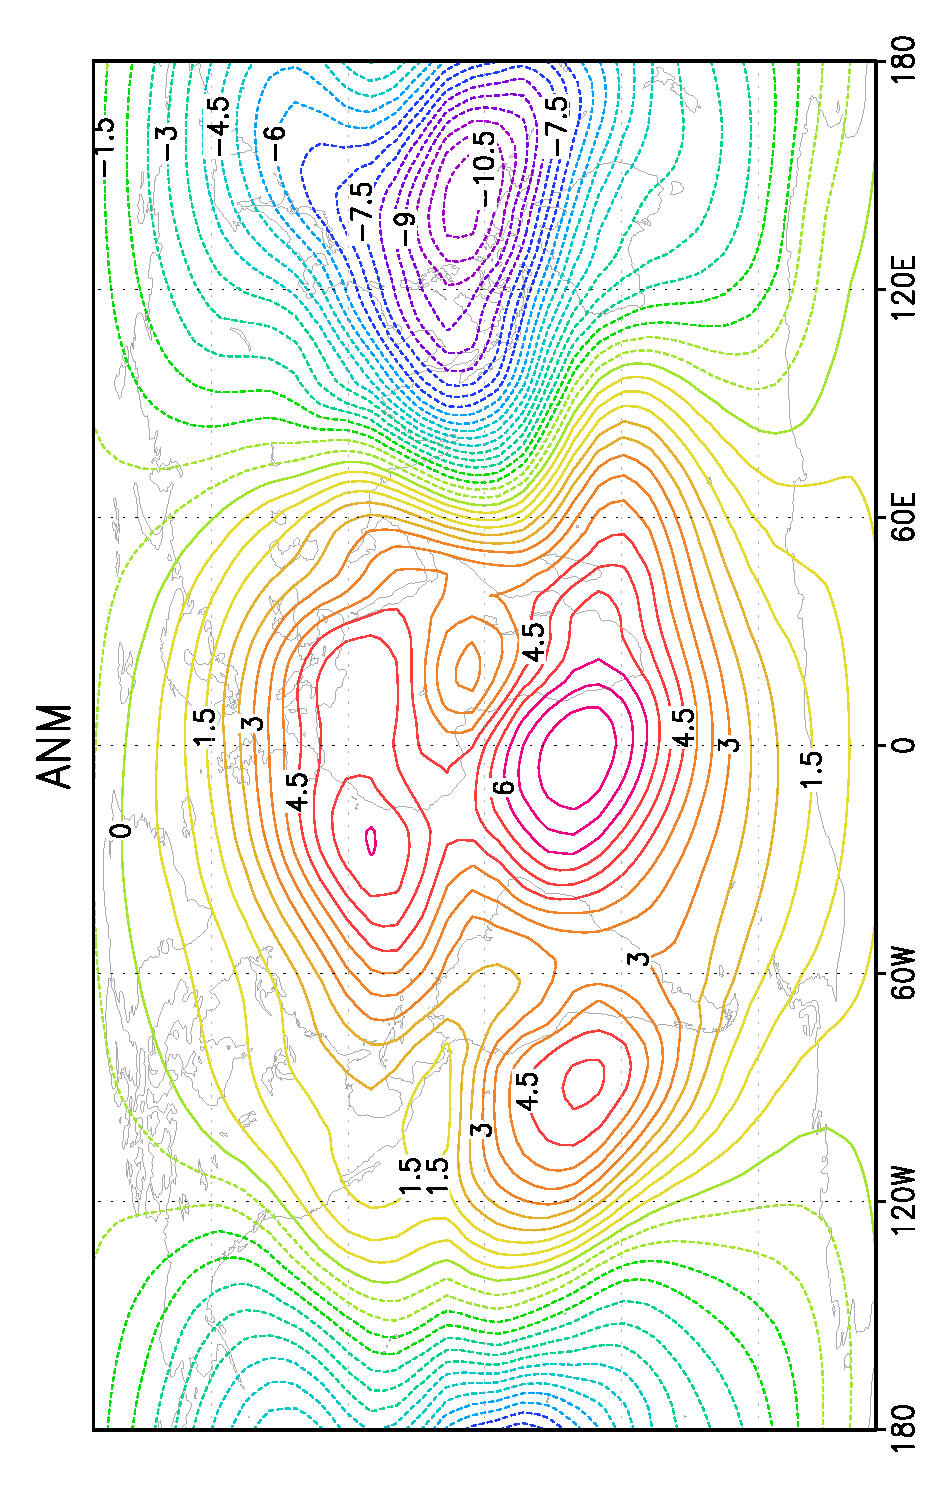
\includegraphics[height=8.5cm,width=6.1cm,angle=-90]
{eps/finaltmt21_ERA40VELPOT200.eps}
}
\caption[Velocity potential at 200 hPa]{Velocity potential $[10^{6}m^{2}/s]$ at 200 hPa}
\label{img:velopot200}
\end{figure}

\vspace{-0.4cm}
\chapter{Radiation}
\vspace{-0.4cm}

The solar and terrestrial radiative fluxes at the top of the atmosphere and at the surface are presented. The surface net radiation enters the Budyko-Lettau dryness ratio (Fig. \ref{img:budyko} on page \pageref{img:budyko}) used for climate classification. 

\vspace{-0.4cm}
\section{Net top solar radiation}
\vspace{-0.4cm}
 
For NH winter (Fig. \ref{img:solrad} a, d), PlaSim and ERA show the same spatial pattern of the shortwave radiation at the top of the atmosphere with maxima near 30° S. Discrepancy occurs north of 70° N where the net balance is close to zero in PlaSim while ERA shows solar radiation, which is due to interpolation. During JJA (Fig. \ref{img:solrad} b, e), the differences are analogue with largest deviations over the SH polar latitudes.


\vspace{-0.4cm}
\section{Net top terrestrial radiation (OLR)}
\vspace{-0.4cm}

In NH winter (Fig. \ref{img:thermrad} a, d), the outgoing long-wave radiation (OLR) shows maxima of -300 $W/m^2$ over tropical oceans and N-Africa slowly decreasing polewards (less negative values). Three main convection areas in the tropics are recognised by PlaSim and ERA with minimum (weaker) values of -240 $W/m^2$: over Indonesia/New Guinea, S-America and Africa. The spatial extension differs between PlaSim and ERA with a weaker minimum in the PlaSim eastern Pacific. In PlaSim and ERA, low values of about -200 $W/m^2$ occur also over the Tibetan Plateau and China caused by low temperatures and minimum cloud cover and not due to enhanced convection. During NH summer (Fig. \ref{img:thermrad} b, e), the structures are again similar in PlaSim and ERA. The values have increased up to\\ -240 $W/m^2$ over the Tibetan Plateau and China caused by enhanced cloud cover during Asian Summer Monsoon. Over the main convection regions in Indonesia/New Guinea, S-America, Africa and the adjacent oceans the OLR increases up to -300 $W/m^2$. In NH summer, the main convective regions (OLR with weaker negative values) shift slightly to the north and are located north of the equator over Central America, Africa and Eastern Asia, which is shown by both PlaSim and ERA; also maximum (strong negative) OLR values (correspond to weak convection) occur over the SH tropics. The main convection region extends to 20° N in PlaSim and ERA and, northward from there (except over Asia), the negative OLR values increase again in N-America, some parts of the Atlantic, N-Africa and southern Europe. North of 60° N, the OLR-values are decreasing again. The zonal means show good agreement between PlaSim and ERA in both seasons. Compared to \citet{Gates1999}, the OLR tends to be overestimated in the tropics by PlaSim, so that the convection is underestimated.


\vspace{-0.4cm}
\section{Net surface solar radiation}
\vspace{-0.4cm}

The NH winter net surface solar radiation (\ref{img:sfcsolrad} a, d) reveals similar spatial patterns for PlaSim and ERA with maxima in the tropics west of S-America, Africa and Australia; here PlaSim shows slightly higher maxima (PlaSim: 330 $W/m^2$, ERA: 300 $W/m^2$). The largest differences are obvious in the polar regions, where PlaSim receives almost no solar radiation north of 60° N. Over the N-Pole, the zonal mean solar radiation vanishes north of 70° N in PlaSim, where ERA-data are affected by the interpolation scheme. Over the S-Pole, PlaSim receives more radiation than ERA. In general, PlaSim solar surface radiation is smaller over the NH (larger over SH) than in ERA. During NH summer (Fig. \ref{img:sfcsolrad} b, e), the differences are analogue. PlaSim has much higher values over large parts of Asia and N-America and over smaller parts to the west of N-Africa (PlaSim: 300 $W/m^2$, ERA: 240 $W/m^2$). PlaSim simulates rather high values of solar radiation over the whole NH tropics extending up to 60° N, which is only partly shown by ERA, where minima occur over Africa and Asia. Therefore, zonal means differ with PlaSim showing a distinct maximum at 30° N, which does not appear in ERA. In contrast, ERA shows higher values over the SH, mainly in the tropics. South of 70° S, the differences between PlaSim and ERA are again due to interpolation.

\vspace{-0.4cm}
\section{Net surface terrestrial radiation}
\vspace{-0.4cm}

In NH winter, the net surface terrestrial radiation shows similar spatial patterns for PlaSim (Fig. \ref{img:sfcthermrad} a) and ERA (Fig. \ref{img:sfcthermrad} d) with maxima (strongest negative values) in the NH. The largest values occur in N-Europe, the NH tropics between 20° to 30° N, and over the warm regions of Australia, S-America and Africa. The largest PlaSim-ERA difference appears in the NH polar regions where PlaSim produces less terrestrial radiation (see cold bias). During JJA (Fig. \ref{img:sfcthermrad} b), the regions with a maximum in thermal radiation remain unchanged. They have merely shifted slightly northwards on the NH. Over the SH, they remain nearly constant as well. Compared to ERA (Fig. \ref{img:thermrad} e), the spatial structures are similar over most regions; larger differences are found near the poles. The N-Pole attains larger, the S-Pole less terrestrial radiation in PlaSim.

\vspace{-0.4cm}
\section{Net top radiation}
\vspace{-0.4cm}

In NH winter, the net top radiation reveals similar spatial patterns for PlaSim and ERA (Fig. \ref{img:netrad} a, d) with the largest values between 10° N and nearly 60° S. Maxima occur over the SH, mainly in the south of S-America, S-Africa and Australia. In these regions and between 30° and 60° S, PlaSim constantly shows higher values (PlaSim: 150 $W/m^2$, ERA: 120 $W/m^2$) whereas in ERA, the net top radiation already decreases south of 30° S. During NH summer (Fig. \ref{img:netrad} b, e), the differences are analogue. The regions with maximum values occur between 10° S and nearly 60° N, mainly to the west of N-America and over the southern parts of Asia. Compared to ERA, PlaSim again shows the higher values and the strongest differences occur over S-Asia (PlaSim: 120 $W/m^2$, ERA: 30 $W/m^2$) and north of 50° N, where the net top radiation is already decreasing in ERA (PlaSim: 90 $W/m^2$, ERA: 30 $W/m^2$ or even less).


\vspace{-0.4cm}
\section{Net surface radiation}
\vspace{-0.4cm}

In NH winter (Fig. \ref{img:sfcnetrad} a, d), the spatial pattern of the net surface radiation is very similar for PlaSim and ERA. The largest values occur between 15° N and 60° S with the maxima located to the west of S-America, S-Africa and Australia. The largest PlaSim-ERA difference only occurs in the spatial extension of the region showing largest values but not in the maxima themselves which correspond well to each other. During NH summer (Fig. \ref{img:sfcnetrad} b, e), high values of the net surface radiation are located between 60° N and 15° S with the maxima to the west of N-America and Africa. Again, this region of high values is more extended in PlaSim. The largest differences between PlaSim and ERA are occurring over Africa and Asia where PlaSim is constantly simulating higher values (PlaSim: about 150 $W/m^2$, ERA: 100 $W/m^2$). 


\begin{figure}[H]
\hspace{3.0cm}PlaSim \vspace{0.2cm}\hspace{7.2cm} ERA \\
\parbox{8.5cm}{\hspace{0.50cm}\begin{scriptsize}(a)\end{scriptsize} \vspace{-0.7cm} \\
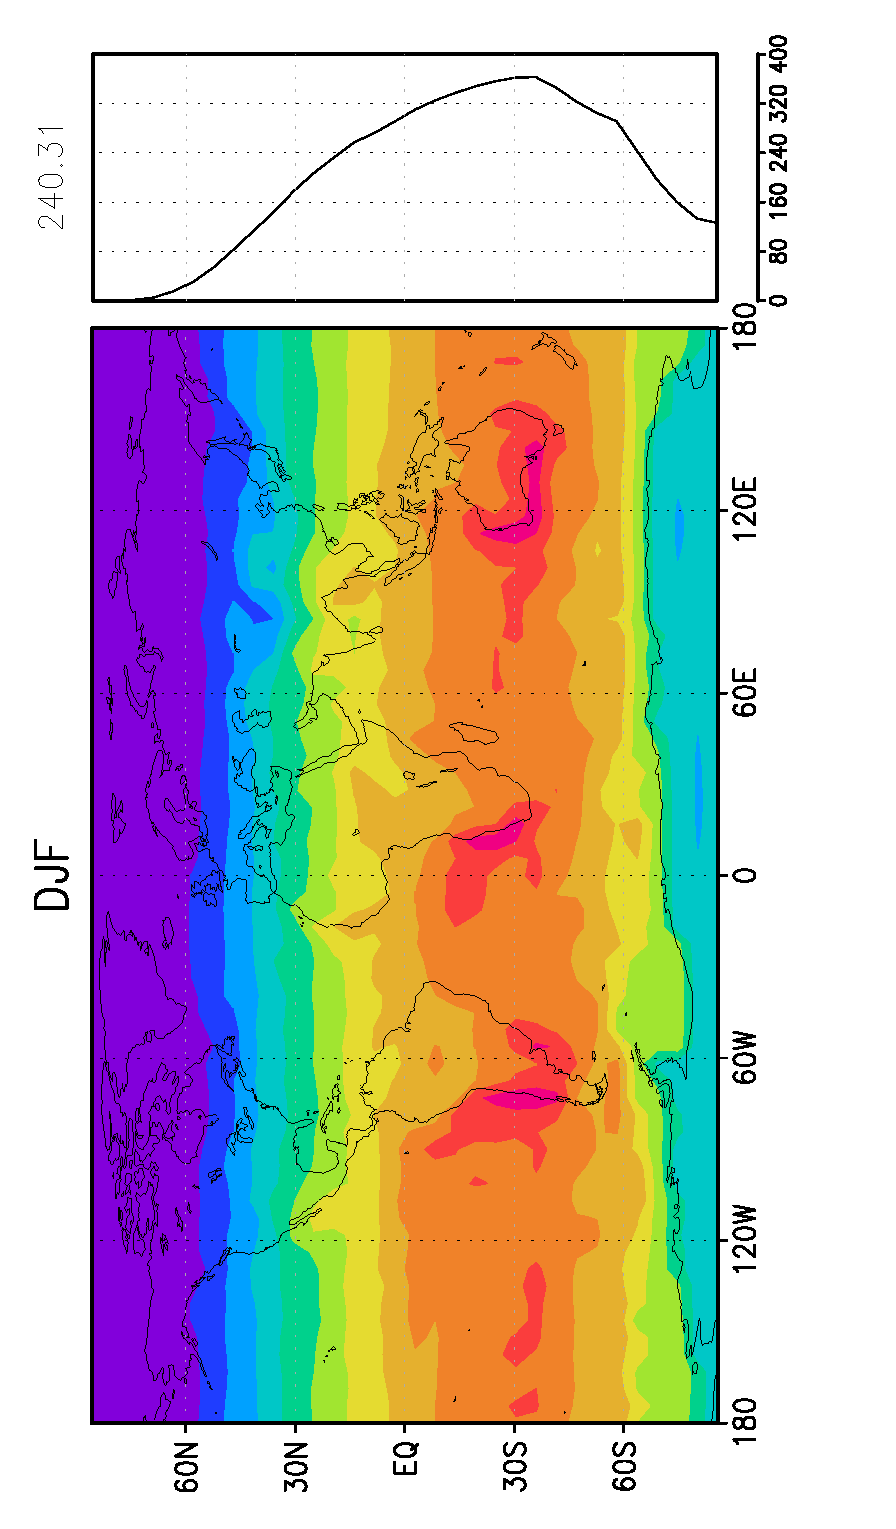
\includegraphics[height=8.5cm,width=6.5cm,angle=-90]
{eps/zonalysmsolrad178DJF.eps}
}
\parbox{8.5cm}{\hspace{0.26cm}\begin{scriptsize}(d)\end{scriptsize} \vspace{-0.7cm} \\
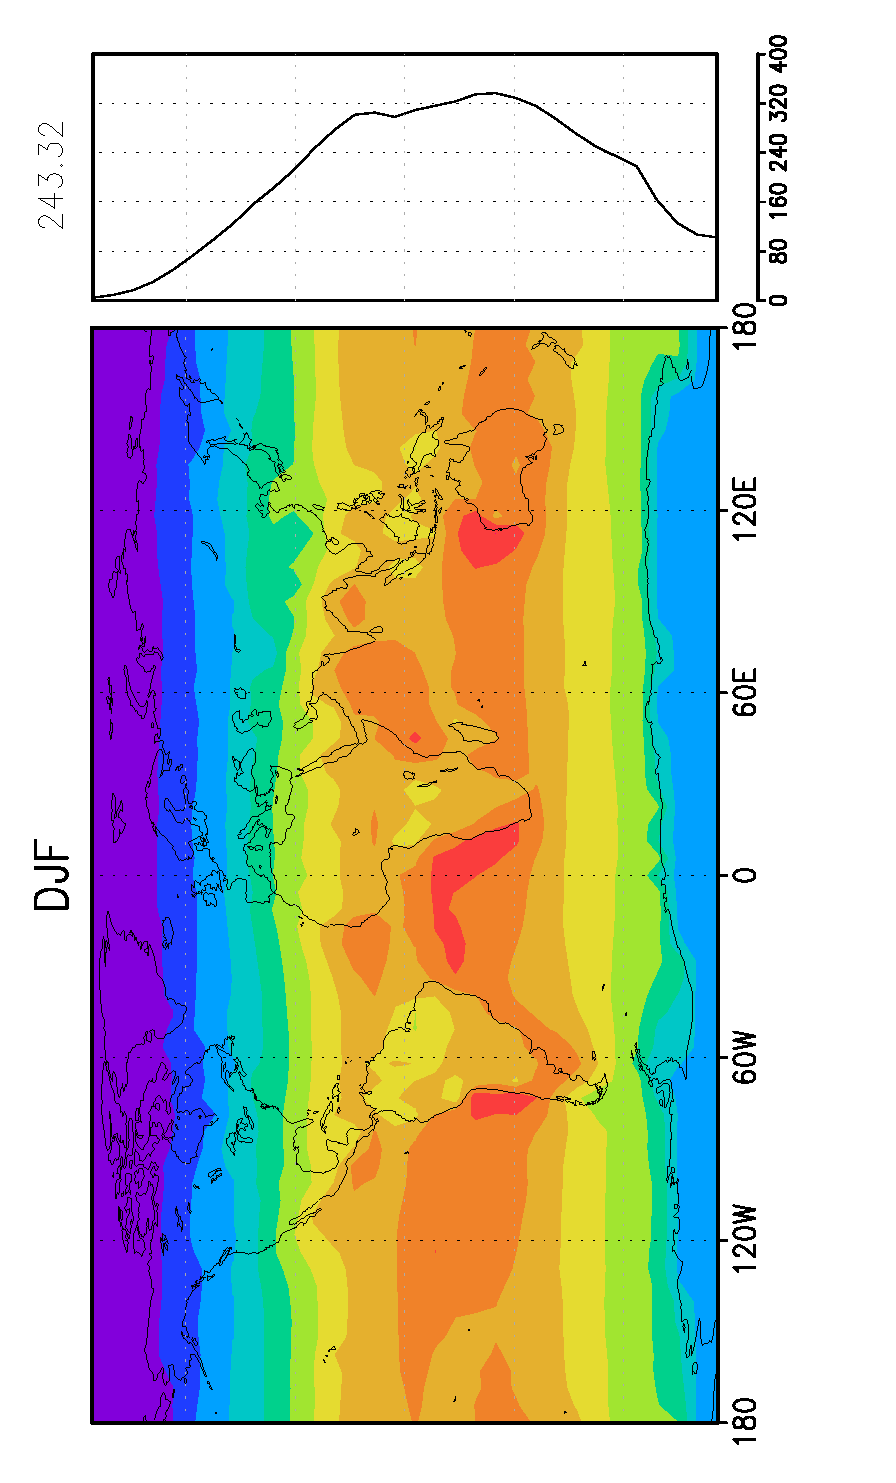
\includegraphics[height=8.5cm,width=6.5cm,angle=-90]
{eps/zonalt21ysmsolradDJF.eps}
}
\parbox{8.5cm}{\hspace{0.50cm}\begin{scriptsize}(b)\end{scriptsize} \vspace{-0.7cm} \\
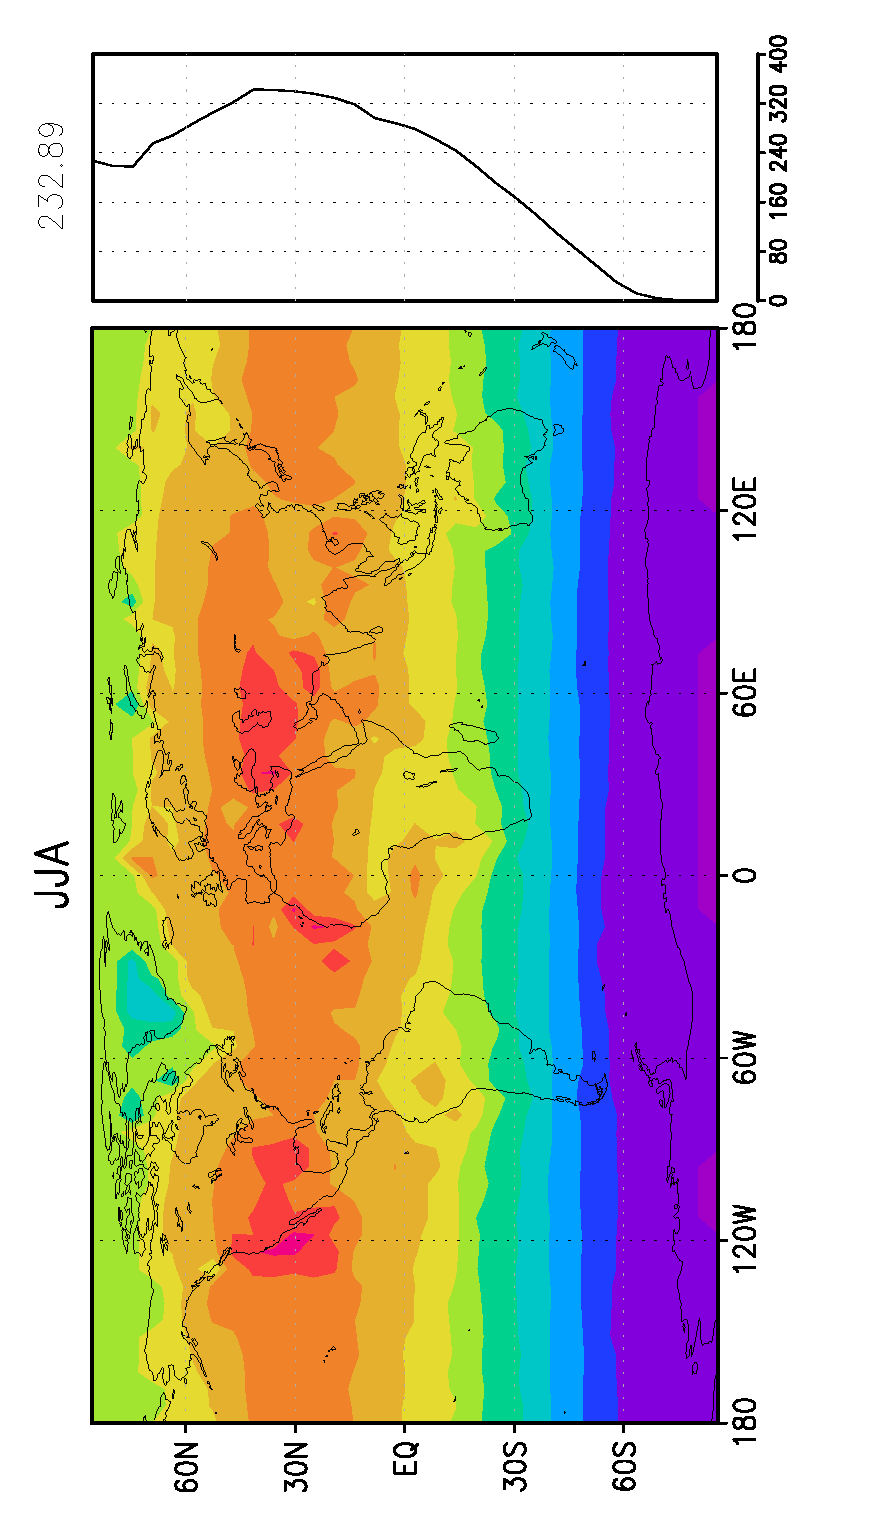
\includegraphics[height=8.5cm,width=6.5cm,angle=-90]
{eps/zonalysmsolrad178JJA.eps}
}
\parbox{8.5cm}{\hspace{0.26cm}\begin{scriptsize}(e)\end{scriptsize} \vspace{-0.7cm} \\
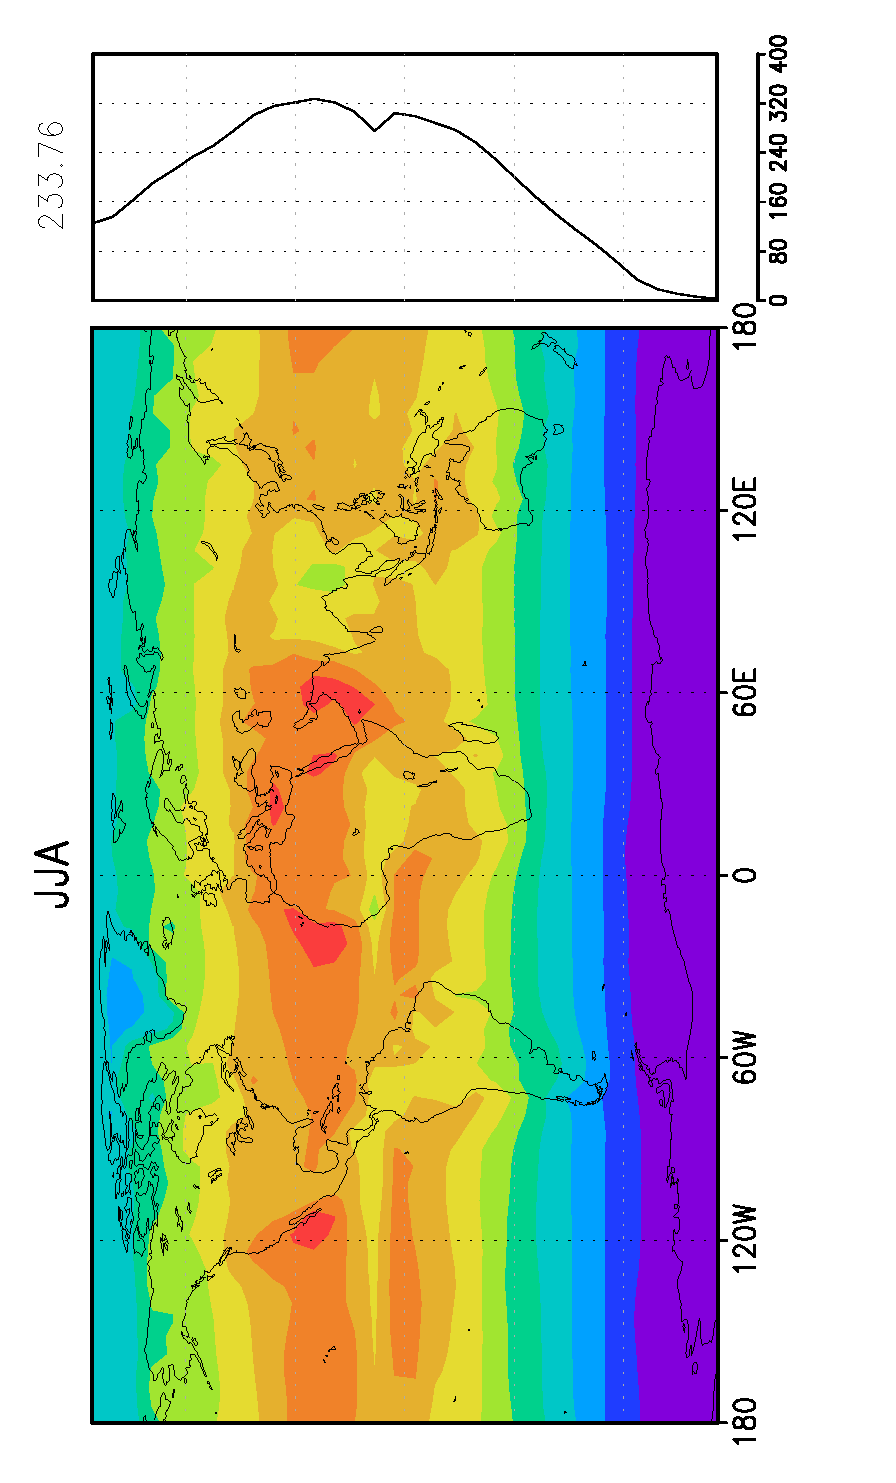
\includegraphics[height=8.5cm,width=6.5cm,angle=-90]
{eps/zonalt21ysmsolradJJA.eps}
}
\parbox{8.4cm}{\hspace{0.50cm}\begin{scriptsize}(c)\end{scriptsize} \vspace{-0.7cm} \\
\includegraphics[height=8.5cm,width=6.5cm,angle=-90]
{eps/zonaltmsolrad178.eps}
}
\parbox{8.5cm}{\hspace{0.48cm}\begin{scriptsize}(f)\end{scriptsize} \vspace{-0.7cm} \\
\includegraphics[height=8.5cm,width=6.5cm,angle=-90]
{eps/zonalt21tmsolrad.eps}
}
\caption[Top solar radiation]{Top solar radiation $[W/m^2]$, positive downward; right panels: zonal mean with global mean on top}
\label{img:solrad}
\end{figure}


\begin{figure}[H]
\hspace{3.0cm}PlaSim \vspace{0.2cm}\hspace{7.2cm} ERA \\
\parbox{8.5cm}{\hspace{0.50cm}\begin{scriptsize}(a)\end{scriptsize} \vspace{-0.7cm} \\
\includegraphics[height=8.5cm,width=6.5cm,angle=-90]
{eps/zonalysmthermrad179DJF.eps}
}
\parbox{8.5cm}{\hspace{0.26cm}\begin{scriptsize}(d)\end{scriptsize} \vspace{-0.7cm} \\
\includegraphics[height=8.5cm,width=6.5cm,angle=-90]
{eps/zonalt21ysmthermradDJF.eps}
}
\parbox{8.5cm}{\hspace{0.50cm}\begin{scriptsize}(b)\end{scriptsize} \vspace{-0.7cm} \\
\includegraphics[height=8.5cm,width=6.5cm,angle=-90]
{eps/zonalysmthermrad179JJA.eps}
}
\parbox{8.5cm}{\hspace{0.26cm}\begin{scriptsize}(e)\end{scriptsize} \vspace{-0.7cm} \\
\includegraphics[height=8.5cm,width=6.5cm,angle=-90]
{eps/zonalt21ysmthermradJJA.eps}
}
\parbox{8.5cm}{\hspace{0.50cm}\begin{scriptsize}(c)\end{scriptsize} \vspace{-0.7cm} \\
\includegraphics[height=8.5cm,width=6.5cm,angle=-90]
{eps/zonaltmthermrad179.eps}
}
\parbox{8.5cm}{\hspace{0.28cm}\begin{scriptsize}(f)\end{scriptsize} \vspace{-0.7cm} \\
\includegraphics[height=8.5cm,width=6.5cm,angle=-90]
{eps/zonalt21tmthermrad.eps}
}
\caption[Net top terrestrial radiation (OLR)]{Net top terrestrial radiation (OLR) $[W/m^2]$; right panels: zonal mean with global mean on top}
\label{img:thermrad}
\end{figure}


\begin{figure}[H]
\hspace{3.0cm}PlaSim \vspace{0.2cm}\hspace{7.2cm} ERA \\
\parbox{8.5cm}{\hspace{0.50cm}\begin{scriptsize}(a)\end{scriptsize} \vspace{-0.7cm} \\
\includegraphics[height=8.5cm,width=6.5cm,angle=-90]
{eps/zonalysmsfcsolrad176DJF.eps}
}
\parbox{8.5cm}{\hspace{0.28cm}\begin{scriptsize}(d)\end{scriptsize} \vspace{-0.7cm} \\
\includegraphics[height=8.5cm,width=6.5cm,angle=-90]
{eps/zonalt21ysmsfcsolradDJF.eps}
}
\parbox{8.5cm}{\hspace{0.50cm}\begin{scriptsize}(b)\end{scriptsize} \vspace{-0.7cm} \\
\includegraphics[height=8.5cm,width=6.5cm,angle=-90]
{eps/zonalysmsfcsolrad176JJA.eps}
}
\parbox{8.5cm}{\hspace{0.28cm}\begin{scriptsize}(e)\end{scriptsize} \vspace{-0.7cm} \\
\includegraphics[height=8.5cm,width=6.5cm,angle=-90]
{eps/zonalt21ysmsfcsolradJJA.eps}
}
\parbox{8.4cm}{\hspace{0.50cm}\begin{scriptsize}(c)\end{scriptsize} \vspace{-0.7cm} \\
\includegraphics[height=8.5cm,width=6.5cm,angle=-90]
{eps/zonaltmsfcsolrad176.eps}
}
\parbox{8.5cm}{\hspace{0.45cm}\begin{scriptsize}(f)\end{scriptsize} \vspace{-0.7cm} \\
\includegraphics[height=8.5cm,width=6.5cm,angle=-90]
{eps/zonalt21tmsfcsolrad.eps}
}
\caption[Net surface solar radiation]{Net surface solar radiation $[W/m^2]$, positive downward; right panels: zonal mean with global mean on top}
\label{img:sfcsolrad}
\end{figure}


\begin{figure}[H]
\hspace{3.0cm}PlaSim \vspace{0.2cm}\hspace{7.2cm} ERA \\
\parbox{8.5cm}{\hspace{0.50cm}\begin{scriptsize}(a)\end{scriptsize} \vspace{-0.7cm} \\
\includegraphics[height=8.5cm,width=6.5cm,angle=-90]
{eps/zonalysmsfcthermrad177DJF.eps}
}
\parbox{8.5cm}{\hspace{0.28cm}\begin{scriptsize}(d)\end{scriptsize} \vspace{-0.7cm} \\
\includegraphics[height=8.5cm,width=6.5cm,angle=-90]
{eps/zonalt21ysmsfcthermradDJF.eps}
}
\parbox{8.5cm}{\hspace{0.50cm}\begin{scriptsize}(b)\end{scriptsize} \vspace{-0.7cm} \\
\includegraphics[height=8.5cm,width=6.5cm,angle=-90]
{eps/zonalysmsfcthermrad177JJA.eps}
}
\parbox{8.5cm}{\hspace{0.28cm}\begin{scriptsize}(e)\end{scriptsize} \vspace{-0.7cm} \\
\includegraphics[height=8.5cm,width=6.5cm,angle=-90]
{eps/zonalt21ysmsfcthermradJJA.eps}
}
\parbox{8.5cm}{\hspace{0.50cm}\begin{scriptsize}(c)\end{scriptsize} \vspace{-0.7cm} \\
\includegraphics[height=8.5cm,width=6.5cm,angle=-90]
{eps/zonaltmsfcthermrad177.eps}
}
\parbox{8.5cm}{\hspace{0.28cm}\begin{scriptsize}(f)\end{scriptsize} \vspace{-0.7cm} \\
\includegraphics[height=8.5cm,width=6.5cm,angle=-90]
{eps/zonalt21tmsfcthermrad.eps}
}
\caption[Net surface terrestrial radiation]{Net surface terrestrial radiation $[W/m^2]$; right panels: zonal mean with global mean on top}
\label{img:sfcthermrad}
\end{figure}


\begin{figure}[H]
\hspace{3.0cm}PlaSim \vspace{0.2cm}\hspace{7.2cm} ERA \\
\parbox{8.5cm}{\hspace{0.50cm}\begin{scriptsize}(a)\end{scriptsize} \vspace{-0.7cm} \\
\includegraphics[height=8.5cm,width=6.5cm,angle=-90]
{eps/zonalysmnetradDJF.eps}
}
\parbox{8.5cm}{\hspace{0.50cm}\begin{scriptsize}(d)\end{scriptsize} \vspace{-0.7cm} \\
\includegraphics[height=8.5cm,width=6.5cm,angle=-90]
{eps/zonalfinalt21ysmnetradDJF.eps}
}
\parbox{8.5cm}{\hspace{0.50cm}\begin{scriptsize}(b)\end{scriptsize} \vspace{-0.7cm} \\
\includegraphics[height=8.5cm,width=6.5cm,angle=-90]
{eps/zonalysmnetradJJA.eps}
}
\parbox{8.5cm}{\hspace{0.50cm}\begin{scriptsize}(e)\end{scriptsize} \vspace{-0.7cm} \\
\includegraphics[height=8.5cm,width=6.5cm,angle=-90]
{eps/zonalfinalt21ysmnetradJJA.eps}
}
\parbox{8.5cm}{\hspace{0.50cm}\begin{scriptsize}(c)\end{scriptsize} \vspace{-0.7cm} \\
\includegraphics[height=8.5cm,width=6.5cm,angle=-90]
{eps/zonaltmnetrad.eps}
}
\parbox{8.5cm}{\hspace{0.50cm}\begin{scriptsize}(f)\end{scriptsize} \vspace{-0.7cm} \\
\includegraphics[height=8.5cm,width=6.5cm,angle=-90]
{eps/zonalt21tmnetrad.eps}
}
\caption[Net top radiation]{Net top radiation $[W/m^2]$; right panels: zonal mean with global mean on top}
\label{img:netrad}
\end{figure}



\begin{figure}[H]
\hspace{3.0cm}PlaSim \vspace{0.2cm}\hspace{7.3cm} ERA \\
\parbox{8.5cm}{\hspace{0.50cm}\begin{scriptsize}(a)\end{scriptsize} \vspace{-0.7cm} \\
\includegraphics[height=8.5cm,width=6.5cm,angle=-90]
{eps/zonalysmsfcnetradDJF.eps}
}
\parbox{8.5cm}{\hspace{0.50cm}\begin{scriptsize}(d)\end{scriptsize} \vspace{-0.7cm} \\
\includegraphics[height=8.5cm,width=6.5cm,angle=-90]
{eps/zonalfinalt21ysmsfcnetradDJF.eps}
}
\parbox{8.5cm}{\hspace{0.50cm}\begin{scriptsize}(b)\end{scriptsize} \vspace{-0.7cm} \\
\includegraphics[height=8.5cm,width=6.5cm,angle=-90]
{eps/zonalysmsfcnetradJJA.eps}
}
\parbox{8.5cm}{\hspace{0.50cm}\begin{scriptsize}(e)\end{scriptsize} \vspace{-0.7cm} \\
\includegraphics[height=8.5cm,width=6.5cm,angle=-90]
{eps/zonalfinalt21ysmsfcnetradJJA.eps}
}
\parbox{8.5cm}{\hspace{0.50cm}\begin{scriptsize}(c)\end{scriptsize} \vspace{-0.7cm} \\
\includegraphics[height=8.5cm,width=6.5cm,angle=-90]
{eps/zonaltmsfcnetrad.eps}
}
\parbox{8.5cm}{\hspace{0.50cm}\begin{scriptsize}(f)\end{scriptsize} \vspace{-0.7cm} \\
\includegraphics[height=8.5cm,width=6.5cm,angle=-90]
{eps/zonalt21tmsfcnetrad.eps}
}
\caption[Net surface radiation]{Net surface radiation $[W/m^2]$; right panels: zonal mean with global mean on top}
\label{img:sfcnetrad}
\end{figure}


\vspace{-0.4cm}
\chapter{Precipitation, evaporation and surface sensible heat flux}
\vspace{-0.4cm}

The water and sensible heat fluxes at the surface complement the balance of the surface energy fluxes. The surface net radiation and precipitation define the Budyko dryness ratio often used for climate and vegetation classification (cf. chapter \ref{classi}); latent and sensible heat fluxes yield the Bowen ratio (Fig. \ref{img:bowen} on page \pageref{img:bowen}); precipitation minus evaporation provides the net fresh water input into the ocean including the terrestrial runoff and, latitudinally integrated, the meridional atmospheric moisture flow is obtained.

\vspace{-0.4cm}
\section{Precipitation}
\vspace{-0.4cm}

NH winter precipitation (Fig. \ref{img:totprec} a, d) in the polar region amounts to 100 mm/season. South of 60° N, precipitation is enhanced mainly over N-America and Asia, and over the adjacent oceans it is increasing up to 600 mm/season. Precipitation minima, besides polar regions, are located over smaller parts of N-America, N-Africa and Asia where hardly any precipitation occurs. While stratiform precipitation prevails in polar regions, south of 10° N convective contribution dominates with maxima in the tropics and south of the equator over S-America, the southern parts of Africa and parts of the Indian and Pacific Ocean. These features are found in PlaSim and ERA. In the equatorial region and southward, ERA shows higher maxima (ERA: about 1800 mm/season, PlaSim: 1200 mm/season). Note that precipitation is overestimated by ERA in the tropics and especially over the oceans \citep{Hagemann2005}. The SH winter structure (Fig. \ref{img:totprec} b, e) shows analogue features: Weak precipitation over polar regions and mid-latitudes. Higher precipitation rates over the Pacific and Atlantic ocean are smaller in PlaSim while ERA has 600 mm/season. In contrast, PlaSim shows higher rates over some parts of N-America, Asia and eastern parts of India and China. Besides the latter regions, the maxima in both data sets are located over the Caribbean and the adjacent Atlantic Ocean as well as equatorial Africa. Except the eastern parts of Africa, which show a precipitation minima, further to the East there is the huge and extensive region influenced by the Asian Summer Monsoon showing maximum precipitation rates. These are mainly located over the Indian Ocean, India itself and parts of Eastern Asia and China respectively. This structure is similar in PlaSim and ERA but PlaSim is continuously showing the lower maxima (PlaSim: 800 mm/season, ERA: about 1600 mm/season), over the continents and over the oceans, but precipitation is overestimated by ERA in this season as well \citep{Hagemann2005}. In the zonal pattern for JJA, there are larger differences between PlaSim and ERA. However, the general pattern is shown by both. PlaSim simulates a larger maximum in about 70° N (PlaSim: about 400 mm/season, ERA: 150 mm/season). In contrast, ERA shows much larger precipitation rates in the NH tropics with a strong peak at about 10° N (ERA: 1000 mm/season, PlaSim: 500 mm/season) which is not simulated by PlaSim. South of the equator, ERA shows a distinct minimum at about 10° S which is weaker in the PlaSim simulation. The subtropical maximum at about 40° S is again more similar in PlaSim and ERA.


\vspace{-0.4cm}
\section{Evaporation}
\vspace{-0.4cm}

In NH winter (Fig. \ref{img:evap} a, d), evaporation shows minima of about 100 mm/season over the continents north of the equator, except some regions of Africa and Central and S-America. Higher evaporation (between 500 to 600 mm/season) is found in the tropics and the adjacent oceans with maxima in the mid-latitude Pacific and Atlantic east of the continents. PlaSim simulates some regions with higher evaporation (about 700 mm/season) over S-America and Africa. During NH summer (Fig. \ref{img:evap} b, e), evaporation increases over large parts of N-America and Africa but decreases over the adjacent oceans, S-America and Africa. Summer evaporation decreases in regions with winter maxima. PlaSim tends to overestimate the evaporation compared to ERA.

\vspace{-0.4cm}
\section{Precipitation minus evaporation}
\vspace{-0.4cm}

The NH winter precipitation minus evaporation or (P-E)-fields show similar spatial patterns (\ref{img:pe} a, d) for PlaSim and ERA with generally small values in the polar regions and larger values in mid-latitudes. While in the tropics the spatial patterns are similar, higher values in ERA are due to overestimated precipitation \citep{Hagemann2005}. In NH summer (Fig. \ref{img:pe} b, e), the spatial patterns are also similar for PlaSim and ERA over the NH and SH mid-latitudes. Again largest differences are obvious in the tropics. The meridional profile for ERA shows a peak near 10° N (not simulated by PlaSim), which may possibly be due to the ERA bias, likewise the SH minimum at 10° S (PlaSim: about -200 mm/season, ERA: about -300 mm/season). The annual mean (Fig. \ref{img:pe} c, f) shows strongest differences in the tropics for PlaSim and ERA while there is good agreement in mid-latitudes of both hemispheres. PlaSim simulates weaker maxima and minima and a much lower global mean. 

\vspace{-0.4cm}
\section{Surface sensible heat flux}
\vspace{-0.4cm}

In NH winter (Fig. \ref{img:sshfl} a, d), the sensible heat flux is most pronounced over land with maximum values in the dry mountainous regions. Largest values occur over N-America, Canada, Asia and the polar regions, where ERA shows continuously high values and PlaSim only partially. At the N-Pole, the sensible heat flux is much smaller in PlaSim than in ERA. The minima of the sensible heat flux can be found in the inner tropics and the mid-latitudes for PlaSim and ERA. Additionally, the tropical oceans and parts of the extra-tropics show negative values. Pronounced minima are noticeable in the mid-latitude Pacific and Atlantic east of Asia and N-America, where evaporation is intense, which is stronger in PlaSim than in ERA (PlaSim: -135 $W/m^2$, ERA: -60 $W/m^2$). In NH summer (Fig. \ref{img:sshfl} b, e), the features are less obvious. Maxima are restricted to the polar regions of the SH, although the heat flux is underestimated by PlaSim compared to ERA (30 $W/m^2$ instead of 60 $W/m^2$ in ERA). The spatial patterns are similar over the continents north of the equator where negative values are more pronounced in PlaSim; south of the equator stronger minima occur in ERA and larger differences are noticeable over the oceans south of 30° S with stronger minima in PlaSim. Compared to the NH winter, the large areas of positive heat fluxes are weaker. The latitudinal variation in the zonal profile is captured by both data sets; larger differences between PlaSim and ERA occur mainly in the NH polar regions (north of 60° N) during NH winter. The ERA heat flux at the N-Pole is about 12 $W/m^2$ compared to PlaSim with -2 $W/m^2$. During NH summer, the differences in the zonal means are largest in the SH tropics north of the equator, the mid-latitudes and at the S-Pole.


\begin{figure}[H]
\hspace{2.9cm}PlaSim \vspace{0.2cm}\hspace{7.2cm} ERA \\
\parbox{8.5cm}{\hspace{0.50cm}\begin{scriptsize}(a)\end{scriptsize} \vspace{-0.7cm} \\
\includegraphics[height=8.5cm,width=6.5cm,angle=-90]
{eps/zonalysmtotalprec260DJF.eps}
}
\parbox{8.5cm}{\vspace{-0.4cm}\hspace{0.28cm}\begin{scriptsize}(d)\end{scriptsize} \vspace{-0.7cm} \\
\includegraphics[height=8.5cm,width=6.5cm,angle=-90]
{eps/zonalt21ysmtotalprecDJF.eps}
}
\parbox{8.5cm}{\hspace{0.50cm}\begin{scriptsize}(b)\end{scriptsize} \vspace{-0.7cm} \\
\includegraphics[height=8.5cm,width=6.5cm,angle=-90]
{eps/zonalysmtotalprec260JJA.eps}
}
\parbox{8.5cm}{\hspace{0.28cm}\begin{scriptsize}(e)\end{scriptsize} \vspace{-0.7cm} \\
\includegraphics[height=8.5cm,width=6.5cm,angle=-90]
{eps/zonalt21ysmtotalprecJJA.eps}
}
\parbox{8.4cm}{\hspace{0.50cm}\begin{scriptsize}(c)\end{scriptsize} \vspace{-0.7cm} \\
\includegraphics[height=8.5cm,width=6.5cm,angle=-90]
{eps/zonaltmtotalprec260.eps}
}
\parbox{8.5cm}{\hspace{0.45cm}\begin{scriptsize}(f)\end{scriptsize} \vspace{-0.7cm} \\
\includegraphics[height=8.5cm,width=6.5cm,angle=-90]
{eps/zonalt21tmtotalprec.eps}
}
\caption[Precipitation]{Precipitation [mm/season] for DJF and JJA and [mm/year] for ANM; right panels: zonal mean with global mean on top}
\label{img:totprec}
\end{figure}


\begin{figure}[H]
\hspace{2.9cm}PlaSim \vspace{0.2cm}\hspace{7.2cm} ERA \\
\parbox{8.5cm}{\hspace{0.50cm}\begin{scriptsize}(a)\end{scriptsize} \vspace{-0.7cm} \\
\includegraphics[height=8.5cm,width=6.5cm,angle=-90]
{eps/zonalysmevap182DJF.eps}
}
\parbox{8.5cm}{\hspace{0.30cm}\begin{scriptsize}(d)\end{scriptsize} \vspace{-0.7cm} \\
\includegraphics[height=8.5cm,width=6.5cm,angle=-90]
{eps/zonalt21ysmevapDJF.eps}
}
\parbox{8.5cm}{\hspace{0.50cm}\begin{scriptsize}(b)\end{scriptsize} \vspace{-0.7cm} \\
\includegraphics[height=8.5cm,width=6.5cm,angle=-90]
{eps/zonalysmevap182JJA.eps}
}
\parbox{8.5cm}{\hspace{0.30cm}\begin{scriptsize}(e)\end{scriptsize} \vspace{-0.7cm} \\
\includegraphics[height=8.5cm,width=6.5cm,angle=-90]
{eps/zonalt21ysmevapJJA.eps}
}
\parbox{8.4cm}{\hspace{0.50cm}\begin{scriptsize}(c)\end{scriptsize} \vspace{-0.7cm} \\
\includegraphics[height=8.5cm,width=6.5cm,angle=-90]
{eps/zonaltmevap182.eps}
}
\parbox{8.5cm}{\hspace{0.45cm}\begin{scriptsize}(f)\end{scriptsize} \vspace{-0.7cm} \\
\includegraphics[height=8.5cm,width=6.5cm,angle=-90]
{eps/zonalt21tmevap.eps}
}
\caption[Evaporation]{Evaporation [mm/season] for DJF and JJA and [mm/year] for ANM; right panels: zonal mean with global mean on top}
\label{img:evap}
\end{figure}


\begin{figure}[H]
\hspace{2.9cm}PlaSim \vspace{0.2cm}\hspace{7.2cm} ERA \\
\parbox{8.5cm}{\hspace{0.50cm}\begin{scriptsize}(a)\end{scriptsize} \vspace{-0.7cm} \\
\includegraphics[height=8.5cm,width=6.5cm,angle=-90]
{eps/zonalfinalpluspeDJF.eps}
}
\parbox{8.5cm}{\hspace{0.35cm}\begin{scriptsize}(d)\end{scriptsize} \vspace{-0.7cm} \\
\includegraphics[height=8.5cm,width=6.5cm,angle=-90]
{eps/zonalt21finalpluspeDJF.eps}
}
\parbox{8.5cm}{\hspace{0.50cm}\begin{scriptsize}(b)\end{scriptsize} \vspace{-0.7cm} \\
\includegraphics[height=8.5cm,width=6.5cm,angle=-90]
{eps/zonalfinalpluspeJJA.eps}
}
\parbox{8.5cm}{\hspace{0.35cm}\begin{scriptsize}(e)\end{scriptsize} \vspace{-0.7cm} \\
\includegraphics[height=8.5cm,width=6.5cm,angle=-90]
{eps/zonalt21finalpluspeJJA.eps}
}
\parbox{8.4cm}{\hspace{0.50cm}\begin{scriptsize}(c)\end{scriptsize} \vspace{-0.7cm} \\
\includegraphics[height=8.5cm,width=6.5cm,angle=-90]
{eps/zonaltmpluspe.eps}
}
\parbox{8.5cm}{\hspace{0.45cm}\begin{scriptsize}(f)\end{scriptsize} \vspace{-0.7cm} \\
\includegraphics[height=8.5cm,width=6.5cm,angle=-90]
{eps/zonalt21tmfinalpe.eps}
}
\caption[P-E]{P-E [mm/season] for DJF and JJA and [mm/year] for ANM; right panels: zonal mean with global mean on top}
\label{img:pe}
\end{figure}


\begin{figure}[H]
\hspace{2.9cm}PlaSim \vspace{0.2cm}\hspace{7.2cm} ERA \\
\parbox{8.5cm}{\hspace{0.50cm}\begin{scriptsize}(a)\end{scriptsize} \vspace{-0.7cm} \\
\includegraphics[height=8.5cm,width=6.5cm,angle=-90]
{eps/zonalysmsshflu146DJF.eps}
}
\parbox{8.5cm}{\hspace{0.30cm}\begin{scriptsize}(d)\end{scriptsize} \vspace{-0.7cm} \\
\includegraphics[height=8.5cm,width=6.5cm,angle=-90]
{eps/zonalt21ysmsshfl146DJFfinal.eps}
}
\parbox{8.5cm}{\hspace{0.50cm}\begin{scriptsize}(b)\end{scriptsize} \vspace{-0.7cm} \\
\includegraphics[height=8.5cm,width=6.5cm,angle=-90]
{eps/zonalysmsshflu146JJA.eps}
}
\parbox{8.5cm}{\hspace{0.30cm}\begin{scriptsize}(e)\end{scriptsize} \vspace{-0.7cm} \\
\includegraphics[height=8.5cm,width=6.5cm,angle=-90]
{eps/zonalt21ysmsshfl146JJAfinal.eps}
}
\parbox{8.4cm}{\hspace{0.50cm}\begin{scriptsize}(c)\end{scriptsize} \vspace{-0.7cm} \\
\includegraphics[height=8.5cm,width=6.5cm,angle=-90]
{eps/zonaltmsshflu146.eps}
}
\parbox{8.5cm}{\hspace{0.48cm}\begin{scriptsize}(f)\end{scriptsize} \vspace{-0.7cm} \\
\includegraphics[height=8.5cm,width=6.5cm,angle=-90]
{eps/zonalt21tmsshfl146final.eps}
}
\caption[Surface sensible heat flux]{Surface sensible heat flux [$W/m^{2}$]; right panels: zonal mean with global mean on top}
\label{img:sshfl}
\end{figure}


\vspace{-0.4cm}
\chapter{Geopotential height: means, storm tracks and wavenumber-frequency spectra}
\vspace{-0.4cm}
\section{500 hPa geopotential height and storm tracks}
\vspace{-0.4cm}

Combination of the 500 hPa geopotential height mean and (bandpass filtered) standard deviation provides information on location and intensity of troughs, jets and storm tracks. PlaSim shows basic spatial patterns and intensities as displayed in a NH circumpolar projection. For NH winter, some aspects are noteworthy, compared to ERA (Fig. \ref{img:z500N} a, c): Too strong zonality does not fully represent the stationary wave structure over Europe and N-America in PlaSim; the Arctic Low is shifted to the northern parts of Greenland. Both bandpass filtered maxima over the Pacific and the N-Atlantic are overestimated and the latter is less extended and slightly shifted to the east and south, compared to ERA. However, the  SH-geopotential for DJF (Fig. \ref{img:z500S} a, c) has a large zonally symmetric component both in PlaSim and ERA.\\
Additional information is obtained from the unfiltered and filtered 1000 hPa geopotential height fields (appendix: Fig. \ref{img:z1000DJF}). The PlaSim climatology compares well with ERA and \citet[p. 82]{Roeckner1996}. Some differences are noted: The large bandpass variability (storm track) over the N-Pacific and N-Atlantic is underestimated over the central oceans, compared mainly to \citet[p. 82]{Roeckner1996}, which can be attributed to reduced cyclonic activity and an overestimation of the mean sea level pressure. In the lowpass regime, the typical pattern with maxima over the north-eastern parts of the N-Pacific and N-Atlantic is represented but with a too small intensity (compared to ERA and \citet{Roeckner1996}).


\vspace{-0.4cm}
\section{Wavenumber-frequency spectra (50° N)}
\vspace{-0.4cm}

The wavenumber-frequency spectra of the 500 hPa geopotential height along 50° N provide information about scale dependent contribution of transient eddy variance and the respective eddy phase speed \citep{Fraedrich1978,Dell'Aquila2005}. The propagating wave spectrum (Fig. \ref{img:frepow} b) shows the following peaks (see Lorenz energy cycle on page \pageref{img:lez}): (i) the low frequency-wavenumber range shows eastward and westward propagating waves; (ii) the high frequency-wavenumber domain corresponds to eastward propagating synoptic scale disturbances. While these general features are shown by PlaSim, \citet{Fraedrich1978} point out, that three spectral peaks should be obvious: the eastward propagating long waves at wavenumber 5-6 and a period of 8-10 days, the eastward propagating short waves at wavenumber 7-8 and a period of 4-6 days and the stationary ultralong waves at wavenumber 1-4 and a period of 20-30 days. In fact, the peaks of the eastward propagating long waves and the stationary ultralong waves are much more pronounced in the PlaSim simulation than the peak of the short waves. Moreover, the strength of all peaks is slightly underestimated by PlaSim, compared to ERA (Fig. \ref{img:frepow} d) and \citet{Fraedrich1978}.


\begin{figure}[c]
\hspace{3.1cm}PlaSim \vspace{-0.1cm}\hspace{7.3cm} ERA \\
\parbox{8.5cm}{\hspace{0.02cm}\begin{scriptsize}(a)\end{scriptsize} \vspace{-0.3cm} \\
\includegraphics[height=7.5cm,angle=-90]
{eps/NHz500StdbpDJF.eps}
}
\parbox{8.5cm}{\hspace{0.02cm}\begin{scriptsize}(c)\end{scriptsize} \vspace{-0.3cm} \\
\includegraphics[height=7.5cm,angle=-90]
{eps/NHt21z500StdbpDJF.eps}
}
\parbox{8.5cm}{\hspace{0.02cm}\begin{scriptsize}(b)\end{scriptsize} \vspace{-0.3cm} \\ 
\includegraphics[height=7.5cm,angle=-90]
{eps/NHz500StdbpJJA.eps}
}
\parbox{8.5cm}{\hspace{0.02cm}\begin{scriptsize}(d)\end{scriptsize} \vspace{-0.3cm} \\
\includegraphics[height=7.5cm,angle=-90]
{eps/NHt21z500StdbpJJA.eps}
}
\caption[Northern Hemisphere 500 hPa geopotential mean and bandpass filtered standard deviation]{500 hPa geopotential mean (isolines, contour spacing is 8 dm) [gpdm] and bandpass filtered standard deviation (shaded) [m] from 25° to 90° N}
\label{img:z500N}
\end{figure}



\begin{figure}[c]
\hspace{3.1cm}PlaSim \vspace{-0.1cm} \hspace{7.3cm} ERA \\
\parbox{8.5cm}{\hspace{0.02cm}\begin{scriptsize}(a)\end{scriptsize} \vspace{-0.3cm} \\
\includegraphics[height=7.5cm,angle=-90]
{eps/SHz500StdbpDJF.eps}
}
\parbox{8.5cm}{\hspace{0.02cm}\begin{scriptsize}(c)\end{scriptsize} \vspace{-0.3cm} \\
\includegraphics[height=7.5cm,angle=-90]
{eps/SHt21z500StdbpDJF.eps}
}
\parbox{8.5cm}{\hspace{0.02cm}\begin{scriptsize}(b)\end{scriptsize} \vspace{-0.3cm} \\
\includegraphics[height=7.5cm,angle=-90]
{eps/SHz500StdbpJJA.eps}
}
\parbox{8.5cm}{\hspace{0.02cm}\begin{scriptsize}(d)\end{scriptsize} \vspace{-0.3cm} \\
\includegraphics[height=7.5cm,angle=-90]
{eps/SHt21z500StdbpJJA.eps}
}
\caption[Southern Hemisphere 500 hPa geopotential mean and bandpass filtered standard deviation]{500 hPa geopotential mean (isolines, contour spacing is 8 dm) [gpdm] and bandpass filtered standard deviation (shaded) [m] from 25° to 90° S}
\label{img:z500S}
\end{figure}



\begin{figure}[c]
\hspace{3.8cm}PlaSim \vspace{0.1cm} \hspace{7.3cm} ERA \\
\parbox{8.5cm}{\hspace{0.50cm}\begin{scriptsize}(a)\end{scriptsize} \vspace{-0.5cm} \\
\includegraphics[height=8.5cm,width=6.5cm,angle=-90]
{eps/wave.srv_powerDJF.eps}
}
\parbox{8.5cm}{\hspace{0.52cm}\begin{scriptsize}(c)\end{scriptsize} \vspace{-0.5cm} \\
\includegraphics[height=8.5cm,width=6.5cm,angle=-90]
{eps/DJFERA_Z500_power.eps}
}
\parbox{8.5cm}{\hspace{0.50cm}\begin{scriptsize}(b)\end{scriptsize} \vspace{-0.3cm} \\
\includegraphics[height=8.5cm,width=6.5cm,angle=-90]
{eps/wave.srv_travellingDJF.eps}
}
\parbox{8.5cm}{\hspace{0.52cm}\begin{scriptsize}(d)\end{scriptsize} \vspace{-0.3cm} \\
\includegraphics[height=8.5cm,width=6.5cm,angle=-90]
{eps/DJFERA_Z500_travelling.eps}
}
\caption[Wavenumber-frequency spectra]{Power spectral density of the meridionally averaged (40° to 52° N) daily 500 hPa geopotential [$10^2 m^2$] for DJF; (a) and (c) Total power spectrum, (b) and (d) Propagating waves $(z'^{2}$)}
\label{img:frepow}
\end{figure}


\vspace{-0.4cm}
\chapter{Zonally averaged fluxes: momentum, sensible heat, wave-activity}


\vspace{-0.4cm}
\section{Heat flux}
\vspace{-0.4cm}


Latitude-height cross-sections of zonal mean northward transport of eddy heat flux are presented for DJF and JJA. The general pattern for DJF (Fig. \ref{img:eddyheat} a, c) with the distinct maximum in about 850 hPa at 50° N is shown by PlaSim and ERA but it is overestimated by PlaSim, compared to ERA and \citet[p. 326]{Peixoto1993}. Over the SH, the structures are similar, but they are slightly more pronounced and extended southward in PlaSim. During SH winter (Fig. \ref{img:eddyheat} b, d), the structures are much more pronounced over the SH with the maximum located at about 60° S. However, this is strongly overestimated by PlaSim (-40 $ms^{-1}K$ in PlaSim compared to -20 $ms^{-1}K$ in ERA). Over the NH, lower absolute values occur together with a more uniform total pattern due to the weaker meridional temperature gradient.\\
The NH heat flux in the 850 hPa-level by transient eddies is shown for NH winter (Fig. \ref{img:vT850DJF}). The characteristic structures, compared to ERA and \citet[p. 86]{Roeckner1996}, are shown by PlaSim, especially the maxima to the east of the American and Asian continent (Fig. \ref{img:vT850DJF} a). The interseasonal comparison (not shown) clearly shows the maximum fluxes in the respective winter hemisphere. A distinct regional separation of the bandpass and lowpass filtered regimes is obvious. In the bandpass regime, large heat fluxes in the western parts of the oceans are caused by developing baroclinic eddies, while in the lowpass regime those fluxes over the Bering Sea are associated with blocking-type flow patterns. Compared to ERA (Fig. \ref{img:vT850DJF} d), both maxima in the unfiltered regime are overestimated by PlaSim and the maximum to the east of N-America is shifted eastwards. In the bandpass regime (Fig. \ref{img:vT850DJF} b, e), the overestimation of the Pacific maximum is even stronger in PlaSim, and in the lowpass regime (Fig. \ref{img:vT850DJF} c, f) the structure is more similar between PlaSim and ERA, except the strong maximum over Greenland, which is not shown by ERA.


\vspace{-0.4cm}
\section{Momentum flux}
\vspace{-0.4cm}

Latitude-height cross-sections of zonal mean northward transport of eddy momentum are presented for DJF and JJA. In NH winter (Fig. \ref{img:eddymom} a, c), there is a strong symmetry with a strong maximum over the SH and a weaker one over the NH. Due to the divergence in 15°, the SH maximum is located in about 35° S at the 250 hPa-level, and over the NH, it is slightly shifted southward \citep[p. 256]{Peixoto1993}. The position of the maxima is correctly revealed by both PlaSim and ERA, but the strength of both is slightly underestimated by PlaSim, as well as the momentum flux in the SH polar regions. During SH winter (Fig. \ref{img:eddymom} b, d), the interhemispheric differences are much more pronounced than in DJF. The pattern over the NH has strongly weakened whereas over the SH it has intensified (e.g. PlaSim: 35 $m^{2}s^{-2}$ over the SH compared to 30 $m^{2}s^{-2}$ over the NH in DJF and 45 $m^{2}s^{-2}$ over the SH compared to 20 $m^{2}s^{-2}$ over the NH in JJA). Compared to ERA, PlaSim again underestimates the maxima. Although the polar maximum has intensified in the PlaSim simulation during JJA, it is still weaker than in ERA.\\
The geographical distribution of the simulated meridional momentum flux by transient eddies in the 300 hPa-level is shown in Figure \ref{img:uvDJF} a, d for NH winter. Northward fluxes occur between 30° and 40° N, with maxima located in the central Pacific, over northern parts of N-America and southern Europe. In contrast to ERA, PlaSim does not show this distinct split between the maxima over the central Pacific and northern parts of N-America but simulates a strong maximum to the west of N-America, underestimating the flux over N-America. This becomes even more obvious in the bandpass regime (Fig. \ref{img:uvDJF} b, e). Over the N-Atlantic, the flux is also slightly too weak, compared to ERA and \citet[p. 88]{Roeckner1996}, and the regions with southward fluxes over the northern oceans are less extended. In the lowpass regime (Fig. \ref{img:uvDJF} c, f), the differences are much stronger compared to ERA and \citet[p. 88]{Roeckner1996}), as the pattern in PlaSim is very coarse. The regions of north- and southward fluxes are captured by PlaSim but their strength is strongly underestimated. 



\vspace{-0.4cm}
\section{Transient wave activity (EP) flux}
\vspace{-0.4cm}

The Eliassen Palm flux (EP, \citet{Eliassen1961}) and its divergence are presented for NH winter and summer from 10° to 80° N (Fig. \ref{img:ep} a-d). The vertical and horizontal components represent meridional eddy fluxes of heat and momentum. The upward component of the EP-flux vectors shows that the poleward eddy heat flux is the main contributor in the low and mid-troposphere. The arrows are tilting equatorwards at upper levels indicating momentum convergence near the jet stream region \citep{Peixoto1993}. In both seasons, the divergence in the lower troposphere is strongly underestimated by PlaSim, compared to ERA and mainly compared to \citet{Peixoto1993}. The PlaSim mid-tropospheric convergence is stronger than in ERA, more extended and shifted downwards. Compared to \citet{Peixoto1993}, the strength is similar but still shifted too much to the lower levels. The tilt is not clearly shown by PlaSim, which contributes to the overall underestimation of the EP-flux divergence. 


\vspace{-0.4cm}
\section{Stationary wave activity flux}
\vspace{-0.4cm}

The three-dimensional propagation of stationary wave activity is shown for the NH (Fig. \ref{img:plumbnorth}). This mechanism is a generalization of the Eliassen-Palm relation \citep{Plumb1984} and the flux permits local diagnosis of the three-dimensional circulation \citep{Plumb1984}.\\
The PlaSim wave activity flux for NH winter is shown in Fig. \ref{img:plumbnorth} a. Compared to ERA (Fig. \ref{img:plumbnorth} c) and the Figures in \citet[p. 225]{Plumb1984}, certain similarities are obvious. Two distinct wavetrains are spreading upward, eastward and predominantly equatorward from eastern Asia across the N-Pacific and from eastern N-America across the N-Atlantic. Smaller features are apparent over central and eastern Europe. Comparing the two major wavetrains, it is obvious that the N-Pacific wavetrain is both more intense and extensive than that in the N-Atlantic. Hence, the flux of stationary wave activity into the stratosphere is dominated by the N-Pacific wavetrain which has additionally a more bended structure whereas that over the N-Atlantic is more uniform. However, the maximum of the N-Pacific (N-Atlantic) wavetrain is shifted too far to the west (east) in PlaSim and their strength is strongly underestimated, compared to ERA. During NH summer (Fig. \ref{img:plumbnorth} b), the N-Pacific wavetrain has shifted to the east in PlaSim and is now located mainly over N-America, ranging from the western parts of the N-Pacific to the western parts of the N-Atlantic. The N-Atlantic wavetrain has equally shifted to the east and is now located over the western parts of Asia. Both wavetrains are now much weaker and less pronounced. Compared to ERA (Fig. \ref{img:plumbnorth} d), certain differences are obvious. In PlaSim, both wavetrains are underestimated and ERA still shows two wavetrains over the N-Pacific and N-Atlantic respectively and a third, but smaller one over the eastern parts of Europe. Compared to DJF, the N-Pacific wavetrain is now extended over the whole N-Pacific whereas the pattern of the N-Atlantic one has nearly remained unchanged, except that both wavetrains are weaker than in winter. In both seasons, the horizontal component (arrows) is much weaker in PlaSim. 



\vspace{-0.4cm}
\section{Eulerian mean circulation}
\vspace{-0.4cm}

Meridional-height cross-sections of the Eulerian mean circulation are presented in Figure \ref{img:resi} for NH winter and summer. The residual mean vertical motion is proportional to the rate of diabatic heating and approximately represents the diabatic circulation in the meridional plane, i.e. the circulation in which parcels are diabatically heated (cooled) when rising (sinking), so that their potential temperature adjusts to the local environment \citep{Holton1992}. This residual meridional circulation consists of a single thermally direct overturning in each hemisphere, with the strongest cell in the respective winter hemisphere. This is shown by PlaSim but the cells are less pronounced and their strength is strongly underestimated, compared to ERA and \citet[p. 325]{Holton1992}.



\begin{figure}[c]
\hspace{4.0cm}PlaSim \vspace{0.2cm} \hspace{7.3cm} ERA \\
\parbox{8.5cm}{\hspace{1cm}\begin{scriptsize}(a)\end{scriptsize} \vspace{-0.5cm} \\
\includegraphics[height=8.5cm,width=6.5cm,angle=-90]
{eps/tmDJFheatflux.eps}
}
\parbox{8.5cm}{\hspace{0.90cm}\begin{scriptsize}(c)\end{scriptsize} \vspace{-0.55cm} \\
\includegraphics[height=8.7cm,width=6.35cm,angle=-90]
{eps/heatflux_ERA40_DJF.eps}
}
\parbox{8.5cm}{\hspace{1cm}\begin{scriptsize}(b)\end{scriptsize} \vspace{-0.5cm} \\
\includegraphics[height=8.5cm,width=6.5cm,angle=-90]
{eps/tmJJAheatflux.eps}
}
\parbox{8.5cm}{\hspace{0.90cm}\begin{scriptsize}(d)\end{scriptsize} \vspace{-0.55cm} \\
\includegraphics[height=8.5cm,width=6.35cm,angle=-90]
{eps/heatflux_ERA40_JJA.eps}
}
\caption[Eddy heat flux for DJF and JJA]{Latitude-height cross-section of zonal mean northward transport of eddy heat flux $v'T'$ [$ms^{-1}K$]}
\label{img:eddyheat}
\end{figure}


\begin{figure}[c]
\hspace{4.0cm}PlaSim \vspace{0.2cm} \hspace{7.3cm} ERA \\
\parbox{8.5cm}{\hspace{1.05cm}\begin{scriptsize}(a)\end{scriptsize} \vspace{-0.5cm} \\
\includegraphics[height=8.5cm,width=6.5cm,angle=-90]
{eps/tmDJFmomentumflux.eps}
}
\parbox{8.5cm}{\hspace{0.95cm}\begin{scriptsize}(c)\end{scriptsize} \vspace{-0.55cm} \\
\includegraphics[height=8.7cm,width=6.35cm,angle=-90]
{eps/momentumflux_ERA40_DJF.eps}
}
\parbox{8.5cm}{\hspace{1.05cm}\begin{scriptsize}(b)\end{scriptsize} \vspace{-0.5cm} \\
\includegraphics[height=8.5cm,width=6.5cm,angle=-90]
{eps/tmJJAmomentumflux.eps}
}
\parbox{8.5cm}{\hspace{0.95cm}\begin{scriptsize}(d)\end{scriptsize} \vspace{-0.55cm} \\
\includegraphics[height=8.5cm,width=6.35cm,angle=-90]
{eps/momentumflux_ERA40_JJA.eps}
}
\caption[Eddy momentum flux for DJF and JJA]{Latitude-height cross-section of zonal mean northward transport of eddy momentum flux $u'v'$ [$m^{2}s^{-2}$]}
\label{img:eddymom}
\end{figure}


\begin{figure}[c]
\hspace{4.0cm}PlaSim \vspace{0.2cm} \hspace{7.3cm} ERA \\
\parbox{8.5cm}{\hspace{0.90cm}\begin{scriptsize}(a)\end{scriptsize} \vspace{-0.5cm} \\
\includegraphics[height=8.5cm,width=6.5cm,angle=-90]
{eps/epdjf.eps}
}
\parbox{8.5cm}{\hspace{0.90cm}\begin{scriptsize}(c)\end{scriptsize} \vspace{-0.5cm} \\
\includegraphics[height=8.5cm,width=6.5cm,angle=-90]
{eps/epdjf_era40.eps}
}
\parbox{8.5cm}{\hspace{0.90cm}\begin{scriptsize}(b)\end{scriptsize} \vspace{-0.5cm} \\
\includegraphics[height=8.5cm,width=6.5cm,angle=-90]
{eps/epjja.eps}
}
\parbox{8.5cm}{\hspace{0.90cm}\begin{scriptsize}(d)\end{scriptsize} \vspace{-0.5cm} \\
\includegraphics[height=8.5cm,width=6.5cm,angle=-90]
{eps/epjja_era40.eps}
}
\caption[EP-flux Northern Hemisphere for DJF and JJA]{Northern Hemisphere EP-flux $[10^{15} m^{3}]$ from 10° to 80° N; EP-flux vectors (arrows) and divergence (isolines)}
\label{img:ep}
\end{figure}



\begin{figure}[c]
\hspace{3.8cm}PlaSim \vspace{0.2cm} \hspace{7.3cm} ERA \\
\parbox{8.5cm}{\hspace{0.95cm}\begin{scriptsize}(a)\end{scriptsize} \vspace{-0.5cm} \\
\includegraphics[height=8.0cm,angle=-90]
{eps/north_DJF_PFLX_TMEAN1.eps}
}
\parbox{8.5cm}{\hspace{0.95cm}\begin{scriptsize}(c)\end{scriptsize} \vspace{-0.5cm} \\
\includegraphics[height=8.0cm,angle=-90]
{eps/dailyERA_north_DJF_PFLX_TMEAN.eps}
}
\parbox{8.5cm}{\hspace{0.95cm}\begin{scriptsize}(b)\end{scriptsize} \vspace{-0.5cm} \\
\includegraphics[height=8.0cm,angle=-90]
{eps/north_JJA_PFLX_TMEAN1.eps}
}
\parbox{8.5cm}{\hspace{0.95cm}\begin{scriptsize}(d)\end{scriptsize} \vspace{-0.5cm} \\
\includegraphics[height=8.0cm,angle=-90]
{eps/dailyERA_north_JJA_PFLX_TMEAN.eps}
}
\caption[Activity flux-Northern Hemisphere]{Northern Hemisphere activity flux between 250 and 850 hPa [$m^{2}s^{-2}$]; horizontal component (arrows) and divergence (isolines)}
\label{img:plumbnorth}
\end{figure}


\begin{figure}[c]
\hspace{4.1cm}PlaSim \vspace{0.2cm} \hspace{7.5cm} ERA \\
\parbox{8.5cm}{\hspace{1.05cm}\begin{scriptsize}(a)\end{scriptsize} \vspace{-0.5cm} \\
\includegraphics[height=8.5cm,width=6.5cm,angle=-90]
{eps/NEWtmDJFresidual.eps}
}
\parbox{8.5cm}{\hspace{1.05cm}\begin{scriptsize}(c)\end{scriptsize} \vspace{-0.55cm} \\
\includegraphics[height=8.7cm,width=6.5cm,angle=-90]
{eps/ERA_NEWDJFresidual.eps}
}
\parbox{8.5cm}{\hspace{1.05cm}\begin{scriptsize}(b)\end{scriptsize} \vspace{-0.5cm} \\
\includegraphics[height=8.5cm,width=6.5cm,angle=-90]
{eps/NEWtmJJAresidual.eps}
}
\parbox{8.5cm}{\hspace{1.05cm}\begin{scriptsize}(d)\end{scriptsize} \vspace{-0.55cm} \\
\includegraphics[height=8.7cm,width=6.5cm,angle=-90]
{eps/ERA_NEWJJAresidual.eps}
}
\caption[Residual mean meridional streamfunction]{Residual mean meridional streamfunction [$hPa*m/s$]}
\label{img:resi}
\end{figure}




\begin{figure}[c]
\hspace{3.5cm}PlaSim \vspace{0.2cm} \hspace{7.3cm} ERA \\
\parbox{8.5cm}{\hspace{0.90cm}\begin{scriptsize}(a)\end{scriptsize} \vspace{-0.5cm} \\
\includegraphics[height=7.5cm,angle=-90]
{eps/PLDJF850fluxes_tr.eps}
}
\parbox{8.5cm}{\hspace{0.95cm}\begin{scriptsize}(d)\end{scriptsize} \vspace{-0.5cm} \\
\includegraphics[height=7.5cm,angle=-90]
{eps/ERADJF850fluxes_tr.eps}
}
\parbox{8.5cm}{\hspace{0.90cm}\begin{scriptsize}(b)\end{scriptsize} \vspace{-0.2cm} \\
\includegraphics[height=7.5cm,angle=-90]
{eps/PLDJF850fluxes_bp.eps}
}
\parbox{8.5cm}{\hspace{0.95cm}\begin{scriptsize}(e)\end{scriptsize} \vspace{-0.2cm} \\
\includegraphics[height=7.5cm,angle=-90]
{eps/ERADJF850fluxes_bp.eps}
}
\parbox{8.5cm}{\hspace{0.90cm}\begin{scriptsize}(c)\end{scriptsize} \vspace{-0.2cm} \\
\includegraphics[height=7.5cm,angle=-90]
{eps/PLDJF850fluxes_lp.eps}
}
\parbox{8.5cm}{\hspace{0.95cm}\begin{scriptsize}(f)\end{scriptsize} \vspace{-0.2cm} \\
\includegraphics[height=7.5cm,angle=-90]
{eps/ERADJF850fluxes_lp.eps}
}
\caption[Eddy heat flux at 850 hPa for DJF and JJA]{Eddy heat flux [$ms^{-1}K$] at 850 hPa from 15° to 90° N for DJF; (a) and (d) unfiltered, (b) and (e) bandpass filtered, (c) and (f) lowpass filtered}
\label{img:vT850DJF}
\end{figure}


\begin{figure}[c]
\hspace{3.5cm}PlaSim \vspace{0.2cm} \hspace{7.3cm} ERA \\
\parbox{8.5cm}{\hspace{0.90cm}\begin{scriptsize}(a)\end{scriptsize} \vspace{-0.5cm} \\
\includegraphics[height=7.5cm,angle=-90]
{eps/PLDJF300fluxes_tr.eps}
}
\parbox{8.5cm}{\hspace{0.95cm}\begin{scriptsize}(d)\end{scriptsize} \vspace{-0.5cm} \\
\includegraphics[height=7.5cm,angle=-90]
{eps/ERADJF300fluxes_tr.eps}
}
\parbox{8.5cm}{\hspace{0.90cm}\begin{scriptsize}(b)\end{scriptsize} \vspace{-0.2cm} \\
\includegraphics[height=7.5cm,angle=-90]
{eps/PLDJF300fluxes_bp.eps}
}
\parbox{8.5cm}{\hspace{0.95cm}\begin{scriptsize}(e)\end{scriptsize} \vspace{-0.2cm} \\
\includegraphics[height=7.5cm,angle=-90]
{eps/ERADJF300fluxes_bp.eps}
}
\parbox{8.5cm}{\hspace{0.90cm}\begin{scriptsize}(c)\end{scriptsize} \vspace{-0.2cm} \\
\includegraphics[height=7.5cm,angle=-90]
{eps/PLDJF300fluxes_lp.eps}
}
\parbox{8.5cm}{\hspace{0.95cm}\begin{scriptsize}(f)\end{scriptsize} \vspace{-0.2cm} \\
\includegraphics[height=7.5cm,angle=-90]
{eps/ERADJF300fluxes_lp.eps}
}
\caption[Eddy momentum flux at 300 hPa for DJF]{Eddy momentum flux [$m^{2}s^{-2}$] at 300 hPa from 15° to 90° N for DJF; (a) and (d) unfiltered, (b) and (e) bandpass filtered, (c) and (f) lowpass filtered}
\label{img:uvDJF}
\end{figure}

\vspace{-0.4cm}
\chapter{Cyclones}
\vspace{-0.4cm}
\section{Mid-latitude cyclones}
\vspace{-0.4cm}

Cyclones are identified as a minimum in the 1000 hPa geopotential height field, which persists for at least two days and shows a minimum mean radial gradient of $30 gpm/1000 km$ \citep{Blender1997}. Cyclone density fields (Figures \ref{img:NHcyclden} and \ref{img:SHcyclden}), derived for PlaSim and ERA, agree in their basic cyclone climatologies, but there are differences: Over the NH, density peaks (winter and summer, see Fig. \ref{img:NHcyclden}) in the N-Atlantic (N-Pacific) are shifted about five to ten degrees southward (northward) in PlaSim (compared to ERA). In NH summer (Fig. \ref{img:NHcyclden} b, d), both peaks are stronger and more zonally oriented, the maximum over the Denmark Strait is overestimated, while the density maxima north of the Persian Gulf, Arabian Sea and Bay of Bengal are underestimated (compared to ERA). The general pattern over the SH (Fig. \ref{img:SHcyclden} a-d) shows a zonal band of cyclonic activity around the Antarctic, which is too extended in PlaSim in summer and winter. In DJF, the maxima in the Atlantic and Indian Ocean are located near 60° S in PlaSim and ERA. The Pacific-maximum should be located between 60° and 70° S \citep{Simmonds2000}, as in ERA, but is shifted about five to ten degrees to the north in PlaSim. During JJA, the density maxima have weakened which is shown by both PlaSim and ERA. One of the more interesting characteristics in lower latitudes, as \citet{Simmonds2000} point out, is the split in the Tasman Sea-New Zealand sector, where low densities occur between 45° and 55° S. This distinct split is not shown by PlaSim, in contrast to ERA and \citet{Simmonds2000}.

\vspace{-0.4cm}
\section{Tropical cyclones}
\vspace{-0.4cm}

The annual mean tropical Cyclone Genesis Parameter (YGP, Fig. \ref{img:sgp} a, b) is the sum of the four Seasonal Genesis Parameter (SGP) for the seasons January-March (JFM), April-June (AMJ), July-September (JAS) and October-November (OND). SGP has been introduced first by \citet{Gray1975} and is used as an empirical tool to infer regions of tropical cyclogenesis \citep{Caron2008}, \citep{Ryan1992}. It is based on six parameters characterising dynamical (Coriolis, low level vorticity, vertical wind shear) and thermodynamic factors (moist static stability, mid-tropospheric moisture, upper ocean temperature). This provides a good predictor of the number of tropical cyclones (TCs) formed in a 5° $\times$ 5° latitude-longitude grid. Figure \ref{img:sgp} a shows the annual mean of the last 20 years of the PlaSim control run. PlaSim correctly shows the regions of TC activity with maxima located over the known hurricane basins in the Atlantic, Indian and Pacific Ocean. Compared to ERA (Fig. \ref{img:sgp} b), the total numbers are slightly underestimated by PlaSim but are still in the range of 10\% less proposed by \citet{Ryan1992}.  



\begin{figure}[c]
\hspace{3.8cm}PlaSim \vspace{0.2cm} \hspace{7.3cm} ERA \\
\parbox{8.5cm}{\hspace{0.95cm}\begin{scriptsize}(a)\end{scriptsize} \vspace{-0.5cm} \\
\includegraphics[height=8.0cm,angle=-90]
{eps/cycldensity_PLASIM_T21_45DJF.eps}
}
\parbox{8.5cm}{\hspace{0.95cm}\begin{scriptsize}(c)\end{scriptsize} \vspace{-0.5cm} \\
\includegraphics[height=8.0cm,angle=-90]
{eps/cycldensity_ERA40_T21_45DJF.eps}
}
\parbox{8.5cm}{\hspace{0.95cm}\begin{scriptsize}(b)\end{scriptsize} \vspace{-0.5cm} \\
\includegraphics[height=8.0cm,angle=-90]
{eps/cycldensity_PLASIM_T21_45JJA.eps}
}
\parbox{8.5cm}{\hspace{0.95cm}\begin{scriptsize}(d)\end{scriptsize} \vspace{-0.5cm} \\
\includegraphics[height=8.0cm,angle=-90]
{eps/cycldensity_ERA40_T21_45JJA.eps}
}
\caption[Cyclone density Northern Hemisphere]{Cyclone density [$\%/1000^2 km^2$] from 20° to 90° N}
\label{img:NHcyclden}
\end{figure}



\begin{figure}[c]
\hspace{3.8cm}PlaSim \vspace{0.2cm} \hspace{7.3cm} ERA \\
\parbox{8.5cm}{\hspace{0.95cm}\begin{scriptsize}(a)\end{scriptsize} \vspace{-0.5cm} \\
\includegraphics[height=8.0cm,angle=-90]
{eps/cycldensity_PLASIM_T21_45DJF_SH.eps}
}
\parbox{8.5cm}{\hspace{0.95cm}\begin{scriptsize}(c)\end{scriptsize} \vspace{-0.5cm} \\
\includegraphics[height=8.0cm,angle=-90]
{eps/cycldensity_ERA40_T21_45DJF_SH.eps}
}
\parbox{8.5cm}{\hspace{0.95cm}\begin{scriptsize}(b)\end{scriptsize} \vspace{-0.5cm} \\
\includegraphics[height=8.0cm,angle=-90]
{eps/cycldensity_PLASIM_T21_45JJA_SH.eps}
}
\parbox{8.5cm}{\hspace{0.95cm}\begin{scriptsize}(d)\end{scriptsize} \vspace{-0.5cm} \\
\includegraphics[height=8.0cm,angle=-90]
{eps/cycldensity_ERA40_T21_45JJA_SH.eps}
}
\caption[Cyclone density Southern Hemisphere]{Cyclone density [$\%/1000^2 km^2$] from 20° to 90° S}
\label{img:SHcyclden}
\end{figure}



\begin{figure}[c]
\begin{tabular}{cc}
\hspace{-0.5cm}PlaSim
\\
\begin{minipage}{1.0\textwidth}
\begin{center}
\begin{scriptsize}(a)\end{scriptsize}\hspace{-1.28cm}\includegraphics[height=16.0cm,angle=-90]{eps/sgpanm.eps}
\end{center}
\end{minipage}
\\
\begin{minipage}{1.0\textwidth}\hspace{7.9cm}ERA\vspace{-0.5cm}
\begin{center}
\begin{scriptsize}(b)\end{scriptsize}\hspace{-1.28cm}\includegraphics[height=16.0cm,angle=-90]{eps/ERAsgpanm.eps}
\end{center}
\end{minipage}
\end{tabular}
\vspace{-1.2cm}\caption[Annual mean Seasonal Genesis Parameter]{Annual mean of the Seasonal Genesis Parameter [cyclones/year] after \citet{Gray1975}}
\label{img:sgp}
\end{figure}


\newpage

\vspace{-0.4cm}
\chapter{Climate Classification}\label{classi}
\vspace{-0.4cm}
\section{Koeppen}
\vspace{-0.4cm}

The Koeppen classification of continental climates (Fig. \ref{img:koeppen} a, b) combines near surface air temperature and precipitation and the respective annual cycle. It thus classifies the world climates by climate state variables combining the thermal energy and water cycle aspects at the surface. Five main climates are distinguished: equatorial (A), arid (B), warm-temperate (C), snow (D) and polar (E); further subclasses are not used here. The five main climates in PlaSim are clearly identified and similar to ERA and to the present day climate respectively \citep{Fraedrich2001}. 

\vspace{-0.4cm}
\section{Budyko-Lettau (dryness ratio)}
\vspace{-0.4cm}

The dryness ratio (D = net radiation/precipitation) characterises the continental surface climates combining long term mean surface energy fluxes to a dimensionless parameter (precipitation enters in terms of its latent energy equivalent). Thus energy limited (D $<$ 1) can be separated from water limited (D $>$ 1) regimes \citep{Budyko1958,Budyko1974,Lettau1969}. Five main climate classes are distinguished: Tundra (0 < D < 0.3), humid savanna to forest (0.3 < D < 1), savanna and steppe (1 < D < 2.3), semi-desert (2.3 < D < 3.4), desert (D > 3.4). The characteristic patterns (Fig. \ref{img:budyko}) are shown by PlaSim and ERA. Larger differences occur over the northern parts of N-America and Asia and smaller parts of S-America, where PlaSim shows a slightly lower dryness ratio than ERA, i.e the region of humid savanna to forest is more extended than in ERA. The dryness ratio is equally underestimated by PlaSim over large parts of N-Africa and Australia, so that the desert is underrepresented there. 


\vspace{-0.4cm}
\section{Bowen ratio}
\vspace{-0.4cm}

The Bowen ratio \citep{Bowen1926a} of surface sensible over latent heat flux (Fig. \ref{img:bowen}) is one of the non-dimensional parameters characterising the near surface climate (see also Budyko-Lettau ratio of dryness, Fig. \ref{img:budyko}). Over the oceans, annual means lie between zero and 0.5 with PlaSim showing considerably higher values (about 0.3 compared to 0.1 for ERA). Over the deserts, PlaSim and ERA provide much larger Bowen ratios due to weak latent heat fluxes but differences occur over N-Africa where PlaSim shows considerably smaller values (about 2 compared to nearly 30 for ERA). Over large parts of Asia, PlaSim simulates higher values, whereas over the American continent, mainly S-America and eastern N-America, and the N-Pole regions, PlaSim strongly underestimates the Bowen ratio, simulating also negative values.




\begin{figure}[c]
\begin{tabular}{cc}
\hspace{-0.5cm}PlaSim \vspace{-0.2cm}
\\
\begin{minipage}{1.0\textwidth}\hspace{1.01cm}\begin{scriptsize}(a)\end{scriptsize} \vspace{-0.05cm}
\begin{center}
\includegraphics[height=8.0cm]{eps/koep_ctrl.eps}
\end{center}
\end{minipage}
\\
\\
\\
\begin{minipage}{1.0\textwidth}\begin{scriptsize}\hspace{1.01cm}(b)\end{scriptsize}\hspace{6.5cm}ERA\vspace{-0.05cm}
\begin{center}
\includegraphics[height=8.0cm]{eps/koep_era.eps}
\end{center}
\end{minipage}
\end{tabular}
\caption[Koeppen climatology]{Koeppen climatology}
\label{img:koeppen}
\end{figure}



\begin{figure}[c]
\begin{tabular}{cc}
\hspace{-0.5cm}PlaSim 
\\
\begin{minipage}{1.0\textwidth}
\begin{center}
\begin{scriptsize}(a)\end{scriptsize}\hspace{-1cm}\includegraphics[height=14.0cm,angle=-90]{eps/budyko_PLAS_ANMnn.eps} 
\end{center}
\end{minipage}
\\
\\
\begin{minipage}{1.0\textwidth}\hspace{7.9cm}ERA\vspace{-0.6cm}
\begin{center}
\begin{scriptsize}(b)\end{scriptsize}\hspace{-1cm}\includegraphics[height=14.0cm,angle=-90]{eps/budyko_ERA40_ANMnn.eps}
\end{center}
\end{minipage}
\end{tabular}
\caption[Annual mean Budyko-Lettau dryness ratio]{Annual mean Budyko-Lettau dryness ratio}
\label{img:budyko}
\end{figure}


\begin{figure}[c]
\begin{tabular}{cc}
\hspace{-0.5cm}PlaSim
\\
\begin{minipage}{1.0\textwidth}
\begin{center}
\begin{scriptsize}(a)\end{scriptsize}\hspace{-1cm}\includegraphics[height=12.0cm,angle=-90]{eps/zonaltmbow.eps} 
\end{center}
\end{minipage}
\\
\\
\begin{minipage}{1.0\textwidth}\hspace{7.9cm}ERA\vspace{-0.6cm}
\begin{center}
\begin{scriptsize}(b)\end{scriptsize}\hspace{-1cm}\includegraphics[height=12.0cm,angle=-90]{eps/zonalt21tmbowen.eps}
\end{center}
\end{minipage}
\end{tabular}
\caption[Bowen ratio]{Annual mean Bowen ratio}
\label{img:bowen}
\end{figure}

\vspace{-0.4cm}
\chapter{Summary and Conclusion}
\vspace{-0.4cm}
In the previous chapters the performance of the Planet Simulator is shown by means of the energetics, the seasonal and annual mean climates of state variables, eddy fluxes and global surface climates. The most important results are now briefly summarised:\\
(i) The global energetics of PlaSim, expressed in the energy and water budgets and the Lorenz energy cycle, show good agreement with observations (\citet{Kiehl1997}, \citet{Trenberth2006} and \citet{Peixoto1993}) and only smaller deviations.\\  
(ii) The seasonal mean climate of the mean sea level pressure shows only small deviations compared to ERA concerning the position and strength of the main pressure systems. Likewise, the general wind pattern shows small deficiencies in the position and the strength of the jets and, although they are both underestimated, PlaSim shows a good structural agreement in terms of the development of the main features of the mass streamfunction and the velocity potential. Larger deviations occur in the temperature and radiation fields, as too less surface and top solar radiation in the winter polar regions are leading to a systematic cold bias there. This is partly due to a deficient prescribed sea ice-distribution, which is extending too far south. This accounts already for half of the total bias, so that the too strong minimum in Fig. \ref{img:surftemp} a in about 80° N is strongly reduced. This new sea-ice distribution is consequently implemented in the new version of the Planet Simulator.\\
Presentation of the global precipitation field shows an even more realistic pattern than in ERA, as the precipitation is strongly overestimated in ERA, mainly in the tropics \citep{Hagemann2005}. Consequently, the P-E-field shows larger differences between PlaSim and ERA as well due to stronger precipitation maxima in ERA.\\ 
(iii) The winter mean of the geopotential height reveals a too strong zonality leading to a deficient stationary wave structure  in PlaSim. Both bandpass filtered maxima over the Pacific and the N-Atlantic are overestimated and the latter is less extended and slightly shifted to the east and south, compared to ERA and \citet[p. 83]{Roeckner1996}. Moreover, the peaks of the wavenumber-frequency spectra of the 500 hPa geopotential height are underestimated by PlaSim as well.\\
(iv) The distribution of the zonally averaged fluxes in PlaSim reveals an opposite picture in PlaSim with a strongly overestimated heat flux and an underestimated momentum flux. This leads to an overall underestimation of the EP-flux divergence and to a deficient tilt of the EP-flux arrows. The stationary wave activity flux shows good structural results but the major wavetrains are strongly underestimated and slightly shifted to the west (east) over the N-Pacific (N-Atlantic). The cells of the residual meridional circulation are less pronounced in PlaSim, and their strength is strongly underestimated, compared to ERA and \citet[p. 325]{Holton1992}.\\
(v) PlaSim shows the basic cyclone climatology patterns of both hemispheres, but the density peaks are shifted southward (northward) in the N-Atlantic (N-Pacific) in both seasons over the NH. During JJA, both peaks are stronger and too zonally oriented, compared to ERA. Moreover, the maximum over the Denmark Strait is overestimated and those over Arabia are strongly underestimated by PlaSim. Over the SH, there is a zonal band of cyclonic activity around the Antarctic, which is too extended in PlaSim in summer and winter. The SH-winter maxima are located in the Atlantic and Indian Ocean near 60° S in both PlaSim and ERA. The Pacific-maximum, which should be located further south, is shifted about five to ten degrees to the north in PlaSim. During NH summer, weaker density maxima occur, as well as a splitted pattern in the Tasman Sea with lower densities further north. PlaSim does not show this split but similar values compared to ERA. In the tropics, PlaSim correctly shows the region of large TC activity, but slightly underestimates the total number of tropical cyclones.\\   
(vi) Finally, PlaSim clearly captures the five main climates of the Koeppen climatology and the Budyko-Lettau dryness ratio.
Compared to ERA, larger differences occur over the northern parts of N-America and Asia and smaller parts of S-America with PlaSim simulating a slightly lower dryness ratio, i.e the region of humid savanna to forest is more extended than in ERA. The desert regions over N-Africa and Australia are less extended as PlaSim equally underestimates the dryness ratio there. Although the main characteristics of the annual mean Bowen ratio are shown by PlaSim, compared to ERA, stronger differences occur over almost all continental regions with PlaSim partly strongly underestimating the Bowen ratio.




























\vspace{-0.4cm}
\chapter{Acknowledgement}
\vspace{-0.4cm}
Part of this work was supported by the DFG Grant FR450/10-1
Cenozoic Antarctic Glaciation:
An Integrated Atmosphere - Ocean - Ice Sheet Model Approach.

\bibliography{report}
\bibliographystyle{agufull}

\listoffigures

\begin{appendix}
\vspace{-0.4cm}
\chapter{Appendix}
\vspace{-0.4cm}
\section{Adjustments of the Planet Simulator}
\vspace{-0.4cm}
In this chapter a detailed overview about the output and the namelists of the PlaSim control run are presented.

\begin{alltt}

 ****************************************************
 * PLANET SIMULATOR     
 ****************************************************
 * NTRU =  21  NLEV =  10  NLON =   64   NLAT =  32 *
 ****************************************************

 **********************************
 * Contents of <surface.txt>      *
 **********************************
 * Code Array name  File position *
 *--------------------------------*
 *  129 doro                   81 *
 *  172 dls                 24994 *
 *  172 yls                 24994 *
 *  172 xls                 24994 *
 *  173 dz0clim             49907 *
 *  174 dalbclim            74820 *
 *  209 dtclsoil            99733 *
 * 1730 dz0climo           124646 *
 *  210 xclicec            149559 *
 *  169 yclsst             448515 *
 *  169 xclsst             448515 *
 *  169 dtcl               448515 *
 *  212 dforest            747471 *
 *  229 dwmax              772384 *
 *  232 dglac              797297 *
 **********************************

 *************************************
 * Namelist INP from <puma_namelist> *
 *************************************
 &INP
 KICK    =           1,
 NWPD    =           1,
 NCOEFF  =           0,
 NDEL    =        10*2,
 NDIAG   =         320,
 NEXP    =           0,
 NEXPER  =           0,
 NKITS   =           3,
 NRESTART=           0,
 NOUTPUT =           1,
 NSTEP   =           0,
 NDEBUG  =           0,
 NTSPD   =          32,
 NEQSIG  =           0,
 NPRINT  =           0,
 NPRHOR  =           0,
 NPACKSP =           1,
 NPACKGP =           1,
 NGUI    =           0,
 NRAD    =           1,
 NFLUX   =           1,
 NTIME   =           1,
 NPERPETUAL  =       0,
 MARS    =           0,
 N_START_YEAR    =   1,
 N_START_MONTH   =   1,
 N_RUN_YEARS     =   1,
 N_RUN_MONTHS    =   0,
 N_RUN_DAYS      =  -1,
 MPSTEP  =          45,
 N_DAYS_PER_MONTH=  30,
 N_DAYS_PER_YEAR = 365,
 DTEP    =  0.0000000E+00,
 DTNS    =  0.0000000E+00,
 DTROP   =   12000.00    ,
 DTTRP   =   2.000000    ,
 TDISSD  = 10*0.2000000  ,
 TDISSZ  = 10*1.100000   ,
 TDISST  = 10*5.600000   ,
 TDISSQ  = 10*5.600000   ,
 TGR     = 288.0000      ,
 PSURF   = 101100.0      ,
 NDL     = 10*0          ,
 NHDIFF  =  15           ,
 RESTIM  = 10*0.0000000E+00  ,
 T0      = 10*250.0000       ,
 TFRC    = 20.00000,100.0000, 8*0.0000000E+00,
 NDIAGGP = 0,
 NDIAGSP = 0,
 NDIAGGP2D =           0,
 NDIAGGP3D =           0,
 NDIAGSP2D =           0,
 NDIAGSP3D =           0,
 NDIAGCF =             0,
 SIGH    = 10*0.0000000E+00  
 /
 ****************************************
 * Namelist PLANET from <puma_namelist> *
 ****************************************
 &PLANET
 AKAP    =  0.2860000    ,
 ALR     =  6.5000001E-03,
 GA      =   9.810000    ,
 GASCON  =   287.0000    ,
 PLARAD  =   6371000.    ,
 PNU     =  0.1000000    ,
 WW      =  7.2921241E-05,
 SOLAR_DAY    =   86400.00,
 SIDERIAL_DAY =   86164.00,
 RA1     =   610.7800    ,
 RA2     =   17.26939    ,
 RA4     =   35.86000    ,
 YPLANET = Earth                           
 /
 Solar day      :  86400.00  [s]
 Siderial day   :  86164.00  [s]
 Timesteps / day:     32
 Timestep       :     45  [min]
 Simulation time:      1  years
 NDEL =            2  Lateral dissipation at lowest level
 with diffusion coefficient =    2336677.94886015 m**2
 e-folding time for smallest scale is    5.600000 days
 Robert time filter with parameter pnu =  0.1000000    

 *********************************
 * Lv *    Sigma Basic-T  Height *
 *********************************
 *  1 *    0.038   0.332  26.105 *
 *  2 *    0.119   0.332  15.724 *
 *  3 *    0.211   0.332  11.453 *
 *  4 *    0.317   0.332   8.446 *
 *  5 *    0.437   0.332   6.084 *
 *  6 *    0.567   0.332   4.169 *
 *  7 *    0.699   0.332   2.626 *
 *  8 *    0.823   0.332   1.428 *
 *  9 *    0.924   0.332   0.580 *
 * 10 *    0.983   0.332   0.124 *
 *********************************


 *********************************************************************
 * Lv * C          1           2           3           4           5 *
 *********************************************************************
 *  1 *   1.00000000  0.00000000  0.00000000  0.00000000  0.00000000 *
 *  2 *   0.67275268  0.32724732  0.00000000  0.00000000  0.00000000 *
 *  3 *   0.37012345  0.41071144  0.21916513  0.00000000  0.00000000 *
 *  4 *   0.24439082  0.27119088  0.31426233  0.17015594  0.00000000 *
 *  5 *   0.17660566  0.19597235  0.22709735  0.26168069  0.13864397 *
 *  6 *   0.13577564  0.15066490  0.17459400  0.20118192  0.22404753 *
 *  7 *   0.10985471  0.12190145  0.14126226  0.16277428  0.18127461 *
 *  8 *   0.09319025  0.10340956  0.11983341  0.13808216  0.15377606 *
 *  9 *   0.08294999  0.09204634  0.10666545  0.12290893  0.13687831 *
 * 10 *   0.07790844  0.08645194  0.10018253  0.11543875  0.12855910 *
 *********************************************************************

 **************************
 * Lv *    Sigma Restor-T *
 **************************
 *  1 *    0.038  210.062 *
 *  2 *    0.119  210.209 *
 *  3 *    0.211  214.963 *
 *  4 *    0.317  231.628 *
 *  5 *    0.437  246.132 *
 *  6 *    0.567  258.603 *
 *  7 *    0.699  269.131 *
 *  8 *    0.823  277.607 *
 *  9 *    0.924  283.763 *
 * 10 *    0.983  287.131 *
 **************************

 white noise added

 *****************************************
 * MISCMOD                               *
 *****************************************
 * Namelist MISCPAR from <puma_namelist> *
 *****************************************
 &MISCPAR
 NFIXER  =           1,
 NUDGE   =           0,
 TNUDGET =   10.00000    
 /

 *****************************************
 * FLUXMOD                               *
 *****************************************
 * Namelist FLUXPAR from <puma_namelist> *
 *****************************************
 &FLUXPAR
 NVDIFF  =           1,
 NSHFL   =           1,
 NEVAP   =           1,
 NSTRESS =           1,
 NTSA    =           2,
 VDIFF_LAMM      =   160.0000    ,
 VDIFF_B =   5.000000    ,
 VDIFF_C =   5.000000    ,
 VDIFF_D =   5.000000    
 /

 ****************************************
 * RADMOD                               *
 ****************************************
 * Namelist RADPAR from <puma_namelist> *
 ****************************************
 &RADPAR
 NDCYCLE =           0,
 NO3     =           1,
 CO2     =   348.0000    ,
 GSOL0   =   1365.000    ,
 IYRBP   =         -50,
 NSWR    =           1,
 NLWR    =           1,
 NFIXORB =           1,
 NSOL    =           1,
 NSWRCL  =           1,
 NRSCAT  =           1,
 RCL1    =  0.1500000,0.3000000, 0.6000000  ,
 RCL2    =  0.1500000,0.3000000,  0.6000000  ,
 ACL2    =  5.0000001E-02,0.1000000,  0.2000000 ,
 CLGRAY  =  -1.000000    ,
 TPOFMT  =   1.000000    ,
 ACLLWR  =  0.1000000    ,
 TSWR1   =  3.4400001E-02,
 TSWR2   =  4.8000000E-02,
 TSWR3   =  4.0000002E-03,
 OZONEFILE       = ozone.dat                                                                       ,
 TH2OC   =  3.9999999E-02,
 DAWN    =  0.0000000E+00
 /
 (orb_params) Use input orbital parameters: 
 (orb_params) ---- Computed Orbital Parameters -----
 (orb_params) Eccentricity      =   1.6714999E-02
 (orb_params) Obliquity (deg)   =  23.44100    
 (orb_params) Obliquity (rad)   =   0.4091226    
 (orb_params) Long of perh(deg) = 102.0000    
 (orb_params) Long of perh(rad) =   4.921828    
 (orb_params) Long at v.e.(rad) =  -3.2612994E-02
 (orb_params) ---------------------------------------

rainmod version

 &RAINPAR
 KBETTA  =           1,
 NPRL    =           1,
 NPRC    =           1,
 NDCA    =           1,
 NCSURF  =           1,
 NMOMENT =           0,
 RCRIT   =  0.9617000,0.8809000,6*0.8500000,0.9240999,0.9833000,
 CLWCRIT1        = -0.1000000    ,
 CLWCRIT2        =  0.0000000E+00
 /

surfmod version

 &SURFPAR
 NSURF   =           1,
 NOROMAX =          21,
 OROSCALE        =   1.000000    ,
 INPUTFILE       = surface_parameter                                                               
 /

 *****************************************
 * LANDMOD                               *
 *****************************************
 * Namelist LANDPAR from <land_namelist> *
 *****************************************
 &LANDPAR
 NLANDT  =   1,
 NLANDW  =   1,
 NBIOME  =   0,
 ALBLAND =  0.2000000    ,
 DZ0LAND =   2.000000    ,
 DRHSLAND=  0.2500000,
 ALBSMIN =  0.4000000    ,
 ALBSMAX =  0.8000000    ,
 ALBSMINF=  0.3000000    ,
 ALBSMAXF=  0.4000000    ,
 ALBGMIN =  0.6000000    ,
 ALBGMAX =  0.8000000    ,
 DSMAX   =   5.000000    ,
 WSMAX   =  0.5000000    ,
 DRHSFULL=  0.4000000    ,
 DZGLAC  =  -1.000000    ,
 DZTOP   =  0.2000000    ,
 DSOILZ  =  0.4000000,0.8000000,1.600000,3.200000,6.400000,
 STARTFILE  = surface_parameter                                                               ,
 RLUE    =  8.0000001E-10,
 CO2CONV =   14.00000    ,
 TAU_VEG =   10.00000    ,
 TAU_SOIL=   42.00000    ,
 FORGROW =   1.000000    ,
 RLAIGROW =  0.5000000   ,
 GS      =   1.000000    ,
 Z0_MAX  =   2.000000    ,
 RINIVEG =  0.0000000E+00,
 RINISOIL =  0.0000000E+00,
 RNBIOCATS=  0.0000000E+00,
 NCVEG   =               1,
 NEWSURF =               0
 /
 SET BIOME PARAMETER
 ===================
 *** array <pgrow> was not in start_data ***
 *** array <plai> was not in start_data ***
 *** array <pgs> was not in start_data ***
 *** array <pz0_max> was not in start_data ***
 *** array <dcveg> was not in start_data ***
 *** array <dcsoil> was not in start_data ***
 Array {dtcl} expanded to 14 months
 *** array <dwcl> was not in surface file ***
 Land:   671 from  2048 =  33%
 Sea:   1377 from  2048 =  67%
 Executing subroutine seaini - Restart = 0
 &SEAPAR
 ALBSEA  =  6.8999998E-02,
 ALBICE  =  0.7000000    ,
 DZ0SEA  =  1.5000000E-05,
 DZ0ICE  =  1.0000000E-03,
 DRHSSEA =   1.000000    ,
 DRHSICE =   1.000000    ,
 NCPL_ATMOS_ICE  =           1
 /
  
 icemod version
  
 &ICEPAR
 NOUT    =          32,
 NFLUKO  =           0,
 NPERPETUAL_ICE  =   0,
 NTSPD   =          32,
 NPRINT  =           0,
 NPRHOR  =           0,
 NICE    =           0,
 NSNOW   =           1,
 NTSKIN  =           1,
 NCPL_ICE_OCEAN  =   1,
 TAUNC   =  0.0000000E+00,
 XMIND   =  0.1000000,
 NEWSURF =           0,
 ICEFILE = surface.txt                                                                     ,
 FLXFILE = ice_flux_correction                                                             
 /
 Array {xclsst} expanded to 14 months
 Array {xclicec} expanded to 14 months
 *** array <xcliced> was not in surface file ***
 ice cover {xclicec} converted from % to fraction
 ice thickness {xcliced} computed from ice cover

 *******************************************
 * OCEANMOD                                *
 *******************************************
 * Namelist OCEANPAR from <ocean_namelist> *
 *******************************************
 &OCEANPAR
 NDIAG   =         480,
 NOUT    =          32,
 NFLUKO  =           0,
 NTSPD   =          32,
 NOCEAN  =           0,
 NPRINT  =           0,
 NPRHOR  =           0,
 NPERPETUAL_OCEAN        =           0,
 TAUNC   =  0.0000000E+00,
 DLAYER  =   50.00000    ,
 VDIFFK  =  9.9999997E-05,
 NEWSURF =           0
 /
 Array {yclsst} expanded to 14 months
 Surface pressure with no topography =    1011.00 [hPa]
 Mean of topographic height          =     231.64 [m]
 Mean of surface pressure            =     983.58 [hPa]


************************************************************
* This simulation is for Earth                             *
************************************************************
*                Parameter       Units     Earth      Mars *
************************************************************
*                     Mass  [10^24 kg]    5.9736    0.6419 *
*                   Volume [10^10 km3]  108.3210   16.3180 *
*        Equatorial radius        [km] 6378.0000 3393.0000 *
*             Polar radius        [km] 6356.0000 3373.0000 *
*              Mean radius        [km] 6371.0000 3390.0000 *
*              Ellipticity                0.0034    0.0065 *
*             Mean density     [kg/m3] 5520.0000 3933.0000 *
*          Surface gravity      [m/s2]    9.8100    3.7400 *
*              Bond albedo                0.3850    0.1600 *
*         Solar irradiance      [W/m2] 1365.0000  595.0000 *
*   Black-body temperature         [K]  247.3000  216.6000 *
*        Topographic range        [km]   20.0000   36.0000 *
*    Sidereal orbit period      [days]  365.2560  686.9800 *
* Sidereal rotation period       [hrs]   23.9345   24.6229 *
*   Equatorial inclination       [deg]   23.4400   23.9800 *
*               Perihelion   [10^6 km]  147.1000  206.6000 *
*                 Aphelion   [10^6 km]  152.1000  249.2000 *
*       Orbit eccentricity                0.0167    0.0934 *
************************************************************
 
Completed month 12-0001
Completed month 12-0001
 *********************************************
  CPU usage in MISCSTEP (ROOT process only):  
     All routines :    2.833282      s
     Fixer        :    2.719276      s
 *********************************************
 *********************************************
  CPU usage in FLUXSTEP (ROOT process only):  
     All routines      :    53.70442      s
     All surface fluxes:    2.626275      s
     Vertical diffusion:    46.32839      s
     Transfere coeff   :  -0.8497211      s
     Sensible heat flux:   -3.406728      s
     Evaporation       :   -2.934723      s
     Wind stress       :   -2.670729      s
 *********************************************
 ******************************************
  CPU usage in RADSTEP (ROOT process only):  
     All routines :    286.7604      s
     Short wave   :    117.2184      s
     Long  wave   :    143.7350      s
 ******************************************
 *********************************************
  CPU usage in RAINSTEP (ROOT process only):  
     All routines   :    107.4204      s
     Large scale p  :    9.982278      s
     Convective p   :    33.47531      s
     Cloud formation:    15.03532      s
     Dry convection :    12.71530      s
 *********************************************
 *******************************************
 *   Run finished at step            23392 *
 *******************************************
 ****************************************************
  total CPU usage (ROOT process only):    747.1870  s
 ****************************************************

ice_namelist

 &ICEPAR
 NICE = 0
 &END

land_namelist
 
 &landpar
 &end

ocean_namelist

 &OCEANPAR
 NOCEAN = 0
 &END

puma_namelist

 &INP
 MARS    =          0
 NOUTPUT =          1
 NGUI    =          0
 N_START_YEAR=      1
 N_DAYS_PER_YEAR= 365
 N_RUN_YEARS=       1
 MPSTEP  =         45
 NWPD    =          1
 NDIAG   =        320
 NPRINT  =          0
 NRESTART =         0
 NTIME    =         1
 &END
 &PLANET
 &END
 &MISCPAR
 &END
 &FLUXPAR
 &END
 &RADPAR
 TSWR1   =     3.44E-2
 NDCYCLE =     0
 NFIXORB =     1
 CO2     =   348.0000
 DAWN    =     0.0000
 GSOL0   =  1365.0000
 &END
 &RAINPAR
 &END
 &SURFPAR
 &END

sea_namelist

&seapar
&end

\end{alltt}

\newpage

\section{Further Output}


\begin{figure}[H]
\hspace{3.1cm}PlaSim \vspace{0.2cm}\hspace{7.1cm} ERA \\
\parbox{8.5cm}{\hspace{0.5cm}\begin{scriptsize}(a)\end{scriptsize} \vspace{-0.5cm} \\
\includegraphics[height=8.5cm,width=6.5cm,angle=-90]
{eps/zonalcelysmT2m167DJF.eps}
}
\parbox{8.5cm}{\hspace{0.25cm}\begin{scriptsize}(d)\end{scriptsize} \vspace{-0.5cm} \\
\includegraphics[height=8.5cm,width=6.5cm,angle=-90]
{eps/zonalcelt21ysmt2mDJF.eps}
}
\parbox{8.5cm}{\hspace{0.5cm}\begin{scriptsize}(b)\end{scriptsize} \vspace{-0.5cm} \\
\includegraphics[height=8.5cm,width=6.5cm,angle=-90]
{eps/zonalcelysmT2m167JJA.eps}
}
\parbox{8.5cm}{\hspace{0.25cm}\begin{scriptsize}(e)\end{scriptsize} \vspace{-0.5cm} \\
\includegraphics[height=8.5cm,width=6.5cm,angle=-90]
{eps/zonalcelt21ysmt2mJJA.eps}
}
\parbox{8.5cm}{\hspace{0.5cm}\begin{scriptsize}(c)\end{scriptsize} \vspace{-0.5cm} \\
\includegraphics[height=8.5cm,width=6.5cm,angle=-90]
{eps/zonalceltmT2m167.eps}
}
\parbox{8.5cm}{\hspace{0.25cm}\begin{scriptsize}(f)\end{scriptsize} \vspace{-0.5cm} \\
\includegraphics[height=8.5cm,width=6.5cm,angle=-90]
{eps/zonalcelt21tmt2m.eps}
}
\caption[T2m]{T2m [°C]. Right panels: zonal mean with global mean on the top.}
\label{img:t2m}
\end{figure}



\begin{figure}[c]
\hspace{4.0cm}PlaSim \vspace{0.2cm} \hspace{7.3cm} ERA \\
\parbox{8.5cm}{\hspace{0.90cm}\begin{scriptsize}(a) \end{scriptsize} \vspace{-0.5cm} \\
\includegraphics[height=8.5cm,width=6.5cm,angle=-90]
{eps/zonysmu_300DJF.eps}
}
\parbox{8.5cm}{\hspace{0.90cm}\begin{scriptsize}(d) \end{scriptsize} \vspace{-0.5cm} \\
\includegraphics[height=8.5cm,width=6.5cm,angle=-90]
{eps/t21zonysmuvel131DJF300.eps}
}
\parbox{8.5cm}{\hspace{0.80cm} \begin{scriptsize}(b) \end{scriptsize} \vspace{-0.5cm} \\
\includegraphics[height=8.5cm,width=6.5cm,angle=-90]
{eps/zonysmu_300JJA.eps}
}
\parbox{8.5cm}{\hspace{0.80cm} \begin{scriptsize}(e) \end{scriptsize} \vspace{-0.5cm} \\
\includegraphics[height=8.5cm,width=6.5cm,angle=-90]
{eps/t21zonysmuvel131JJA300.eps}
}
\parbox{8.5cm}{\hspace{0.80cm} \begin{scriptsize}(c) \end{scriptsize} \vspace{-0.5cm} \\
\includegraphics[height=8.5cm,width=6.5cm,angle=-90]
{eps/zontmu_300.eps}
}
\parbox{8.5cm}{\hspace{0.80cm} \begin{scriptsize}(f) \end{scriptsize} \vspace{-0.5cm} \\
\includegraphics[height=8.5cm,width=6.5cm,angle=-90]
{eps/t21zontmuvel131300.eps}
}
\caption[Zonally averaged zonal wind at 300 hPa]{Zonally averaged zonal wind at 300 hPa [m/s]}
\label{img:uzon300}
\end{figure}


\begin{figure}[c]
\hspace{4.0cm}PlaSim \vspace{0.2cm} \hspace{7.3cm} ERA \\
\parbox{8.5cm}{\hspace{0.90cm}\begin{scriptsize}(a) \end{scriptsize} \vspace{-0.5cm} \\
\includegraphics[height=8.5cm,width=6.5cm,angle=-90]
{eps/zonysmu_850DJF.eps}
}
\parbox{8.5cm}{\hspace{0.90cm}\begin{scriptsize}(d) \end{scriptsize} \vspace{-0.5cm} \\
\includegraphics[height=8.5cm,width=6.5cm,angle=-90]
{eps/t21zonysmuvel131DJF850.eps}
}
\parbox{8.5cm}{\hspace{0.80cm} \begin{scriptsize}(b) \end{scriptsize} \vspace{-0.5cm} \\
\includegraphics[height=8.5cm,width=6.5cm,angle=-90]
{eps/zonysmu_850JJA.eps}
}
\parbox{8.5cm}{\hspace{0.80cm} \begin{scriptsize}(e) \end{scriptsize} \vspace{-0.5cm} \\
\includegraphics[height=8.5cm,width=6.5cm,angle=-90]
{eps/t21zonysmuvel131JJA850.eps}
}
\parbox{8.5cm}{\hspace{0.80cm} \begin{scriptsize}(c) \end{scriptsize} \vspace{-0.5cm} \\
\includegraphics[height=8.5cm,width=6.5cm,angle=-90]
{eps/zontmu_850.eps}
}
\parbox{8.5cm}{\hspace{0.80cm} \begin{scriptsize}(f) \end{scriptsize} \vspace{-0.5cm} \\
\includegraphics[height=8.5cm,width=6.5cm,angle=-90]
{eps/t21zontmuvel131850.eps}
}
\caption[Zonally averaged zonal wind at 850 hPa]{Zonally averaged zonal wind at 850 hPa [m/s]}
\label{img:uzon850}
\end{figure}

\newpage

\begin{figure}[c]
\hspace{3.1cm}PlaSim \vspace{0.2cm} \hspace{7.1cm} ERA \\
\parbox{8.5cm}{\hspace{0.50cm}\begin{scriptsize} (a)\end{scriptsize} \vspace{-0.5cm} \\
\includegraphics[height=8.5cm,width=6.5cm,angle=-90]
{eps/zonalysmslhflu147DJF.eps}
}
\parbox{8.5cm}{\hspace{0.25cm}\begin{scriptsize} (d)\end{scriptsize} \vspace{-0.5cm} \\
\includegraphics[height=8.5cm,width=6.5cm,angle=-90]
{eps/zonalt21ysmslhfl147DJFfinal.eps}
}
\parbox{8.5cm}{\hspace{0.50cm}\begin{scriptsize} (b)\end{scriptsize} \vspace{-0.5cm} \\
\includegraphics[height=8.5cm,width=6.5cm,angle=-90]
{eps/zonalysmslhflu147JJA.eps}
}
\parbox{8.5cm}{\hspace{0.25cm}\begin{scriptsize} (e)\end{scriptsize} \vspace{-0.5cm} \\
\includegraphics[height=8.5cm,width=6.5cm,angle=-90]
{eps/zonalt21ysmslhfl147JJAfinal.eps}
}
\parbox{8.5cm}{\hspace{0.5cm}\begin{scriptsize} (c)\end{scriptsize} \vspace{-0.5cm} \\
\includegraphics[height=8.5cm,width=6.5cm,angle=-90]
{eps/zonaltmslhflu147.eps}
}
\parbox{8.5cm}{\hspace{0.25cm}\begin{scriptsize} (f)\end{scriptsize} \vspace{-0.5cm} \\
\includegraphics[height=8.5cm,width=6.5cm,angle=-90]
{eps/zonalt21tmslhfl147final.eps}
}
\caption[Surface latent heat flux]{Surface latent heat flux [$W/m^{2}$]. Right panels: zonal mean with global mean on the top.}
\label{img:slhfl}
\end{figure}


\begin{figure}[c]
\hspace{3.55cm}PlaSim \vspace{0.2cm} \hspace{7.25cm} ERA \\
\parbox{8.5cm}{\hspace{0.90cm}\begin{scriptsize}(a) \end{scriptsize} \vspace{-0.5cm} \\
\includegraphics[height=7.5cm,angle=-90]
{eps/northcircysmz500DJF.eps}
}
\parbox{8.5cm}{\hspace{0.90cm}\begin{scriptsize}(d) \end{scriptsize} \vspace{-0.5cm} \\
\includegraphics[height=7.5cm,angle=-90]
{eps/northcirct21ysmz500DJF.eps}
}
\parbox{8.5cm}{\hspace{0.80cm} \begin{scriptsize}(b) \end{scriptsize} \vspace{-0.5cm} \\
\includegraphics[height=7.5cm,angle=-90]
{eps/northcircysmz500JJA.eps}
}
\parbox{8.5cm}{\hspace{0.80cm} \begin{scriptsize}(e) \end{scriptsize} \vspace{-0.5cm} \\
\includegraphics[height=7.5cm,angle=-90]
{eps/northcirct21ysmz500JJA.eps}
}
\parbox{8.5cm}{\hspace{0.80cm} \begin{scriptsize}(c) \end{scriptsize} \vspace{-0.5cm} \\
\includegraphics[height=7.5cm,angle=-90]
{eps/northcirctmz500.eps}
}
\parbox{8.5cm}{\hspace{0.80cm} \begin{scriptsize}(f) \end{scriptsize} \vspace{-0.5cm} \\
\includegraphics[height=7.5cm,angle=-90]
{eps/northcirct21tmz500.eps}
}
\caption[z500 Northern Hemisphere]{z500 Northern Hemisphere [gpdm] from 20° to 90° N. Contour spacing is 8 dm.}
\label{img:z500north}
\end{figure}



\begin{figure}[c]
\hspace{3.55cm}PlaSim \vspace{0.2cm} \hspace{7.25cm} ERA \\
\parbox{8.5cm}{\hspace{0.90cm}\begin{scriptsize}(a) \end{scriptsize} \vspace{-0.5cm} \\
\includegraphics[height=7.5cm,angle=-90]
{eps/southcircysmz500DJF.eps}
}
\parbox{8.5cm}{\hspace{0.90cm}\begin{scriptsize}(d) \end{scriptsize} \vspace{-0.5cm} \\
\includegraphics[height=7.5cm,angle=-90]
{eps/southcirct21ysmz500DJF.eps}
}
\parbox{8.5cm}{\hspace{0.80cm} \begin{scriptsize}(b) \end{scriptsize} \vspace{-0.5cm} \\
\includegraphics[height=7.5cm,angle=-90]
{eps/southcircysmz500JJA.eps}
}
\parbox{8.5cm}{\hspace{0.80cm} \begin{scriptsize}(e) \end{scriptsize} \vspace{-0.5cm} \\
\includegraphics[height=7.5cm,angle=-90]
{eps/southcirct21ysmz500JJA.eps}
}
\parbox{8.5cm}{\hspace{0.80cm} \begin{scriptsize}(c) \end{scriptsize} \vspace{-0.5cm} \\
\includegraphics[height=7.5cm,angle=-90]
{eps/southcirctmz500.eps}
}
\parbox{8.5cm}{\hspace{0.80cm} \begin{scriptsize}(f) \end{scriptsize} \vspace{-0.5cm} \\
\includegraphics[height=7.5cm,angle=-90]
{eps/southcirct21tmz500.eps}
}
\caption[z500 Southern Hemisphere]{z500 Southern Hemisphere [gpdm] from 20° to 90° S. Contour spacing is 8 dm.}
\label{img:z500south}
\end{figure}



\begin{figure}[c]
\hspace{3.5cm}PlaSim \vspace{0.2cm} \hspace{7.3cm} ERA \\
\parbox{8.5cm}{\hspace{0.90cm}\begin{scriptsize}(a)\end{scriptsize} \vspace{-0.5cm} \\
\includegraphics[height=7.5cm,angle=-90]
{eps/PLDJF1000z156fluxes_tr.eps}
}
\parbox{8.5cm}{\hspace{0.95cm}\begin{scriptsize}(d)\end{scriptsize} \vspace{-0.5cm} \\
\includegraphics[height=7.5cm,angle=-90]
{eps/ERA40_Z1000DJF_fluxes_tr.eps}
}
\parbox{8.5cm}{\hspace{0.90cm}\begin{scriptsize}(b)\end{scriptsize} \vspace{-0.2cm} \\
\includegraphics[height=7.5cm,angle=-90]
{eps/PLDJF1000z156fluxes_bp.eps}
}
\parbox{8.5cm}{\hspace{0.95cm}\begin{scriptsize}(e)\end{scriptsize} \vspace{-0.2cm} \\
\includegraphics[height=7.5cm,angle=-90]
{eps/ERA40_Z1000DJF_fluxes_bp.eps}
}
\parbox{8.5cm}{\hspace{0.90cm}\begin{scriptsize}(c)\end{scriptsize} \vspace{-0.2cm} \\
\includegraphics[height=7.5cm,angle=-90]
{eps/PLDJF1000z156fluxes_lp.eps}
}
\parbox{8.5cm}{\hspace{0.95cm}\begin{scriptsize}(f)\end{scriptsize} \vspace{-0.2cm} \\
\includegraphics[height=7.5cm,angle=-90]
{eps/ERA40_Z1000DJF_fluxes_lp.eps}
}
\caption[Northern Hemisphere 1000 hPa standard deviation]{Northern Hemisphere 1000 hPa standard deviation [m] from 15° to 90° N for DJF; (a) and (d) unfiltered, (b) and (e) bandpass filtered, (c) and (f) lowpass filtered}
\label{img:z1000DJF}
\end{figure}



\begin{figure}[c]
\hspace{3.8cm}PlaSim \vspace{0.2cm} \hspace{7.3cm} ERA \\
\parbox{8.5cm}{\hspace{0.95cm}\begin{scriptsize}(a)\end{scriptsize} \vspace{-0.5cm} \\
\includegraphics[height=8.0cm,angle=-90]
{eps/cyclgen_PLASIM_T21_45DJF.eps}
}
\parbox{8.5cm}{\hspace{0.95cm}\begin{scriptsize}(c)\end{scriptsize} \vspace{-0.5cm} \\
\includegraphics[height=8.0cm,angle=-90]
{eps/cycldensity_ERA40_T21_45DJF.eps}
}
\parbox{8.5cm}{\hspace{0.95cm}\begin{scriptsize}(b)\end{scriptsize} \vspace{-0.5cm} \\
\includegraphics[height=8.0cm,angle=-90]
{eps/cyclgen_PLASIM_T21_45JJA.eps}
}
\parbox{8.5cm}{\hspace{0.95cm}\begin{scriptsize}(d)\end{scriptsize} \vspace{-0.5cm} \\
\includegraphics[height=8.0cm,angle=-90]
{eps/cycldensity_ERA40_T21_45JJA.eps}
}
\caption[Cyclogenesis density Northern Hemisphere]{Cyclogenesis density [$\%/1000^2 km^2$] from 20° to 90° N}
\label{img:NHyclgen}
\end{figure}


\begin{figure}[c]
\hspace{3.8cm}PlaSim \vspace{0.2cm} \hspace{7.3cm} ERA \\
\parbox{8.5cm}{\hspace{0.95cm}\begin{scriptsize}(a)\end{scriptsize} \vspace{-0.5cm} \\
\includegraphics[height=8.0cm,angle=-90]
{eps/cycllys_PLASIM_T21_45DJF.eps}
}
\parbox{8.5cm}{\hspace{0.95cm}\begin{scriptsize}(c)\end{scriptsize} \vspace{-0.5cm} \\
\includegraphics[height=8.0cm,angle=-90]
{eps/cycllys_ERA40_T21_45DJF.eps}
}
\parbox{8.5cm}{\hspace{0.95cm}\begin{scriptsize}(b)\end{scriptsize} \vspace{-0.5cm} \\
\includegraphics[height=8.0cm,angle=-90]
{eps/cycllys_PLASIM_T21_45JJA.eps}
}
\parbox{8.5cm}{\hspace{0.95cm}\begin{scriptsize}(d)\end{scriptsize} \vspace{-0.5cm} \\
\includegraphics[height=8.0cm,angle=-90]
{eps/cycllys_ERA40_T21_45JJA.eps}
}
\caption[Cyclolysis density Northern Hemisphere]{Cyclolysis density[$\%/1000^2 km^2$] from 20° to 90° N}
\label{img:NHcycllys}
\end{figure}


\begin{figure}[c]
\hspace{3.8cm}PlaSim \vspace{0.2cm} \hspace{7.3cm} ERA \\
\parbox{8.5cm}{\hspace{0.95cm}\begin{scriptsize}(a)\end{scriptsize} \vspace{-0.5cm} \\
\includegraphics[height=8.0cm,angle=-90]
{eps/cyclgen_PLASIM_T21_45DJF_SH.eps}
}
\parbox{8.5cm}{\hspace{0.95cm}\begin{scriptsize}(c)\end{scriptsize} \vspace{-0.5cm} \\
\includegraphics[height=8.0cm,angle=-90]
{eps/cyclgen_ERA40_T21_45DJF_SH.eps}
}
\parbox{8.5cm}{\hspace{0.95cm}\begin{scriptsize}(b)\end{scriptsize} \vspace{-0.5cm} \\
\includegraphics[height=8.0cm,angle=-90]
{eps/cyclgen_PLASIM_T21_45JJA_SH.eps}
}
\parbox{8.5cm}{\hspace{0.95cm}\begin{scriptsize}(d)\end{scriptsize} \vspace{-0.5cm} \\
\includegraphics[height=8.0cm,angle=-90]
{eps/cyclgen_ERA40_T21_45JJA_SH.eps}
}
\caption[Cyclogenesis density Southern Hemisphere]{Cyclogenesis density [$\%/1000^2 km^2$] from 20° to 90° S}
\label{img:SHcyclgen}
\end{figure}


\begin{figure}[c]
\hspace{3.8cm}PlaSim \vspace{0.2cm} \hspace{7.3cm} ERA \\
\parbox{8.5cm}{\hspace{0.95cm}\begin{scriptsize}(a)\end{scriptsize} \vspace{-0.5cm} \\
\includegraphics[height=8.0cm,angle=-90]
{eps/cycllys_PLASIM_T21_45DJF_SH.eps}
}
\parbox{8.5cm}{\hspace{0.95cm}\begin{scriptsize}(c)\end{scriptsize} \vspace{-0.5cm} \\
\includegraphics[height=8.0cm,angle=-90]
{eps/cycllys_ERA40_T21_45DJF_SH.eps}
}
\parbox{8.5cm}{\hspace{0.95cm}\begin{scriptsize}(b)\end{scriptsize} \vspace{-0.5cm} \\
\includegraphics[height=8.0cm,angle=-90]
{eps/cycllys_PLASIM_T21_45JJA_SH.eps}
}
\parbox{8.5cm}{\hspace{0.95cm}\begin{scriptsize}(d)\end{scriptsize} \vspace{-0.5cm} \\
\includegraphics[height=8.0cm,angle=-90]
{eps/cycllys_ERA40_T21_45JJA_SH.eps}
}
\caption[Cyclolysis density Southern Hemisphere]{Cyclolysis density [$\%/1000^2 km^2$] from 20° to 90° S}
\label{img:SHcycllys}
\end{figure}

\end{appendix}


\end{document}
 
 


